\thispagestyle{toancuabinone}
\pagestyle{toancuabi}
\everymath{\color{toancuabi}}
\graphicspath{{../toancuabi/pic/}}
\begingroup
\AddToShipoutPicture*{\put(0,616){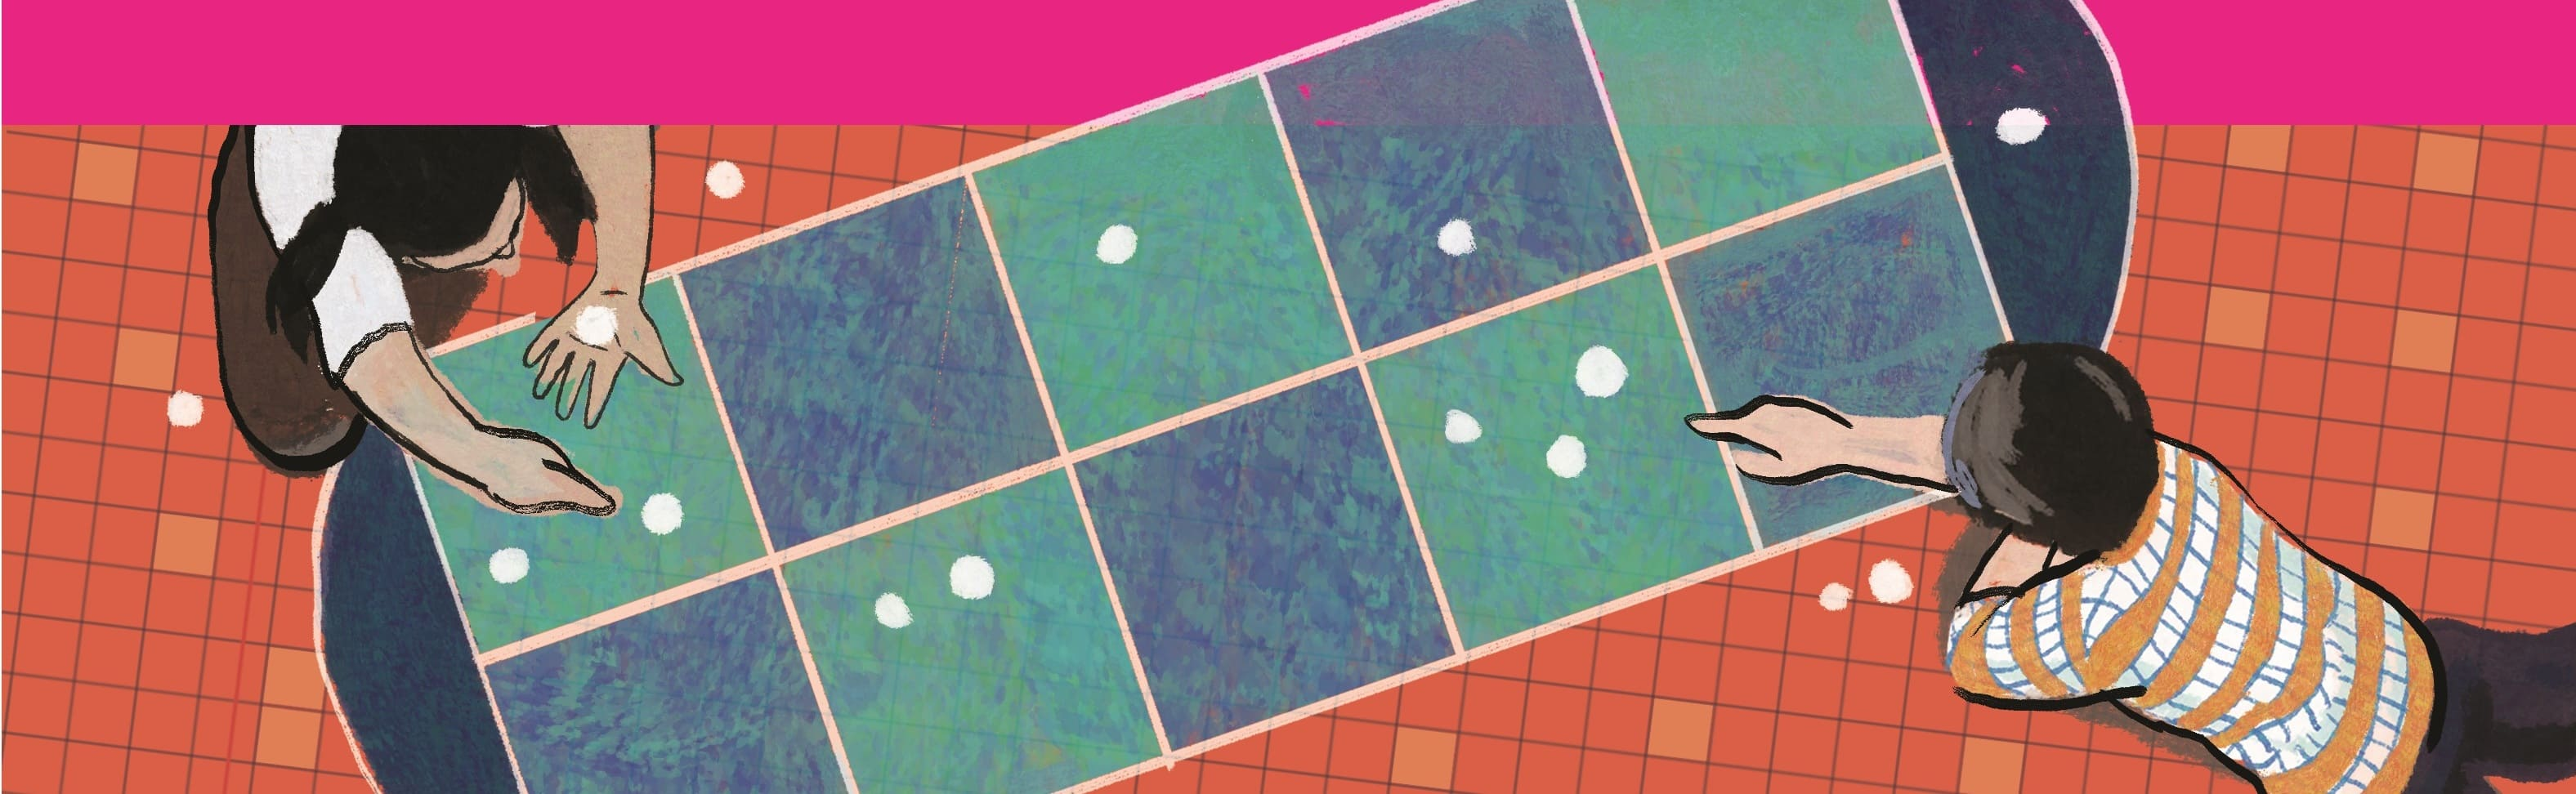
\includegraphics[width=19.3cm]{../bannertoancuabi}}}  
\AddToShipoutPicture*{\put(70,492){
\includegraphics[scale=1]{../tieude1.pdf}}} 
\centering
\endgroup
\vspace*{215pt}

\begin{multicols}{2}
	Trong chương trình phổ thông của Việt Nam, toán tổ hợp đếm được giới thiệu ở cấp THPT. Tuy nhiên trong một số cuộc thi học sinh giỏi toán dành cho cấp tiểu học và đầu cấp PTCS thì phần tổ hợp đếm đã được đưa vào nội dung bài thi khá nhiều, ví dụ như một số cuộc thi khá phổ biến ở Việt Nam hiện nay như IMAS (International Mathematics Assessment), Apmops (The Asia Pacific Mathematical Olympiad for Primary Schools), IMSO (The International Mathematics and Science Olympiad)...
	\vskip 0.1cm
	Trong bài viết này chúng ta cùng làm quen với một số bài toán về đếm tổ hợp trong một số cuộc thi học sinh giỏi cấp tiểu học và lớp $6$ THCS.
	\vskip 0.1cm
	Trước hết chúng ta làm quen với một số khái niệm cơ bản trong phần toán tổ hợp đếm.
	\vskip 0.1cm
	\textbf{\color{toancuabi}Quy tắc cộng, quy tắc nhân:} Quy tắc cộng và quy tắc nhân là hai quy tắc đếm cơ bản, có nội dung có thể được mô tả như sau:
	\vskip 0.1cm
	Có hai công việc gọi là Job $1$ và Job $2$ (có thể mở rộng ra nhiều hơn $2$ công việc) được thực hiện một cách độc lập nhau. Có $m$ cách thực hiện Job $1$ và $n$ cách thực hiện Job $2$, khi đó hai quy tắc đếm cơ bản được phát biểu như sau:
	\vskip 0.1cm
	\textbf{\color{toancuabi}Quy tắc cộng:} Có $m+n$ cách để thực hiện Job $1$ hoặc Job $2$.
	\begin{figure}[H]
		\centering
		\vspace*{-5pt}
		\captionsetup{labelformat=empty, justification=centering}
		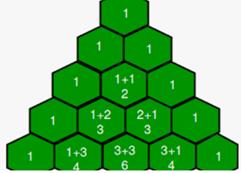
\includegraphics[width=0.85\linewidth]{_1}
		\caption{\small\textit{\color{toancuabi}Quy tắc cộng trong tam giác Pascal.}}
		\vspace*{-10pt}
	\end{figure}
	\textbf{\color{toancuabi}Quy tắc nhân:} Có $m\times n$ cách để thực hiện Job$1$ và Job$2$ (thực hiện cả hai công việc).
	\begin{figure}[H]
		\centering
		\vspace*{-5pt}
		\captionsetup{labelformat=empty, justification=centering}
		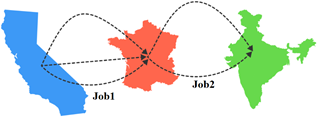
\includegraphics[width=1\linewidth]{_2}
		\caption{\small\textit{\color{toancuabi}Quy tắc nhân trong bài toán đếm đường đi.}}
		\vspace*{-10pt}
	\end{figure}
	\textbf{\color{toancuabi}Giai thừa:} của $n$ là số cách sắp xếp thứ tự của $n$ phần tử trong một tập hợp, được ký hiệu là $n!$ và có công thức là: $n!=1\times 2\times 3\times \ldots\times n $.
	\vskip 0.1cm
	Ghi chú: $0!=1$
	\begin{figure}[H]
		\centering
		\vspace*{5pt}
		\captionsetup{labelformat=empty, justification=centering}
		
\includegraphics[width=1\linewidth]{_3}
		\vspace*{-15pt}
	\end{figure}
	\textbf{\color{toancuabi}Hoán vị (Permutation):} Có $n$ người và chỉ có $k$ cái ghế trên một hàng ($k\le n$), ta cần xếp đủ $k$ người từ nhóm $n$ người vào $k$ cái ghế. Khi đó số cách xếp gọi là hoán vị và ký hiệu là:
	\begin{align*}
		P(n,k)&=n\!\times\!(n\!-\!1)\!\!\times\!\!(n\!-\!2)\!\!\times\!\!\ldots\!\!\times\!\!(n\!-\!k\!+\!1\!)\\
		&= \frac{n!}{(n-k)!} 
	\end{align*}
	\vskip 0.1cm
	Trong trường hợp có $n$ người và có đúng $n$ cái ghế khi đó ta có số cách sắp xếp $n$ người này chính là định nghĩa của $n!$ (số cách sắp xếp các phần tử của một tập hợp $n$ phần tử): $P(n,n)=n!$
	\begin{figure}[H]
		\centering
		\vspace*{-10pt}
		\captionsetup{labelformat=empty, justification=centering}
		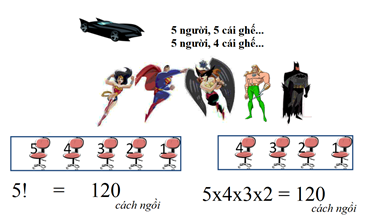
\includegraphics[width=1\linewidth]{_4}
		\vspace*{-15pt}
	\end{figure}
	\resizebox{\columnwidth}{!}{{\textbf{\color{toancuabi}Hoán vị vòng tròn (Circular Permutation):}}} Xung quanh một bàn tròn có $n$ người ngồi. Hai hoán vị được coi là như nhau nếu chúng có thể chồng khít vào nhau bằng phép xuay. Số cách sắp xếp $n$ người xung quanh môt cái bàn tròn cố định là: (\textit{cố định: có nghĩa là ta không thể nhấc nó ra để lật ngược lại được})
	\begin{align*}
		P_n=(n-1)!
	\end{align*}
	Số là $(n-1)!$ thay vì $n!$ vì có $n$ cách xoay bàn và $n$ hoán vị do xoay bàn từ $1$ vị trí là như nhau.
	\begin{figure}[H]
		\centering
		\vspace*{5pt}
		\captionsetup{labelformat=empty, justification=centering}
		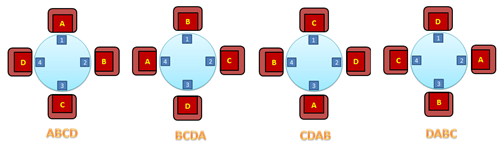
\includegraphics[width=1\linewidth]{_5}
		\caption{\small\textit{\color{toancuabi}Hoán vị vòng tròn $4$ người ngồi xung quanh một cái bàn hình tròn.}}
		\vspace*{-10pt}
	\end{figure}
	\textbf{\color{toancuabi}Tổ hợp (Combonation):}  Đếm số cách để chọn $k$ người từ một nhóm $n$ người là một trong những bài toán tổ hợp đếm cơ bản, và nó được gọi bằng một cái tên đặc biệt: TỔ HỢP và được ký hiệu  $C(n,k)$; $C_n^k$ và có công thức là:
	\begin{align*}
		C_n^k&=C(n,k)=\frac{P(n,k)}{k!} \\[-0.5ex]
		&= \frac{n\!\times\!(n\!-\!1)\!\times\!(n\!-\!2)\!\times\!\ldots \!\times\!(n\!-\!k\!+\!1)}{k!}\\[-0.75ex]
		& = \frac{n!}{k!\times(n-k)!}
	\end{align*}
	\vskip 0.1cm
		\textbf{\color{toancuabi}Bài toán số $\pmb{1}$: (IMAS)}
		\vskip 0.1cm
		Sơ đồ dưới đây gồm nhiều tam giác vuông cân.
		\vskip 0.1cm
		Có bao nhiêu cách một con kiến có thể đi từ $A$ đến $C$ nếu nó chỉ được phép di chuyển lên trên, sang phải hay theo đường chéo? 
		\begin{figure}[H]
			\centering
			\vspace*{-10pt}
			\captionsetup{labelformat=empty, justification=centering}
			\begin{tikzpicture}[toancuabi,scale=0.7]
				\draw  (-4.,0.)-- (0.,0.);
				\draw  (0.,4.)-- (0.,0.);
				\draw  (0.,4.)-- (-4.,0.);
				\draw  (-3.,0.)-- (-3.,1.);
				\draw  (-3.,1.)-- (-2.,1.);
				\draw  (-2.,0.)-- (-2.,2.);
				\draw  (-2.,2.)-- (0.,2.);
				\draw  (-1.,2.)-- (-1.,3.);
				\draw  (-1.,3.)-- (0.,3.);
				\draw  (0.,1.)-- (-1.,1.);
				\draw  (-1.,1.)-- (-1.,0.);
				\draw  (0.,2.)-- (-2.,0.);
				\draw  (0.,1.)-- (-1.,0.);
				\draw  (-2.,1.)-- (-3.,0.);
				\draw  (0.,3.)-- (-1.,2.);
				\draw (-4.36,0.11) node {$A$};
				\draw (0.38,0.09) node {$B$};
				\draw (0.2,4.47) node {$C$};
			\end{tikzpicture}
			\vspace*{-10pt}
		\end{figure}
	\textbf{\color{toancuabi}Phân tích bài toán:} Tại mỗi điểm nút trên hình vẽ, số cách đi từ $A$ đến nó sẽ bằng tổng số cách đi từ $A$ đến các điểm nút ngay đằng trước nó theo chiều mũi tên được phép đi (phải, lên trên và đi chéo).
	\vskip 0.1cm
	Vậy nên ta có để điền mũi tên hướng đi và áp dụng quy tắc cộng để giải quyết các bài toán dạng này.
	\vskip 0.1cm
	\textit{Lời giải}: Theo quy tắc cộng thể hiện trên hình vẽ bên dưới ta có tổng số cách đi từ $A$ đến $C$ là $42$.
	\begin{figure}[H]
		\centering
%		\vspace*{-10pt}
		\captionsetup{labelformat=empty, justification=centering}
		\begin{tikzpicture}[toancuabi,scale=0.7]
			\draw  (-4.,0.)-- (0.,0.);
			\draw  (0.,4.)-- (0.,0.);
			\draw  (0.,4.)-- (-4.,0.);
			\draw  (-3.,0.)-- (-3.,1.);
			\draw  (-3.,1.)-- (-2.,1.);
			\draw  (-2.,0.)-- (-2.,2.);
			\draw  (-2.,2.)-- (0.,2.);
			\draw  (-1.,2.)-- (-1.,3.);
			\draw  (-1.,3.)-- (0.,3.);
			\draw  (0.,1.)-- (-1.,1.);
			\draw  (-1.,1.)-- (-1.,0.);
			\draw  (0.,2.)-- (-2.,0.);
			\draw  (0.,1.)-- (-1.,0.);
			\draw  (-2.,1.)-- (-3.,0.);
			\draw  (0.,3.)-- (-1.,2.);
			
			\draw[-stealth]  (-4.,0.)-- (-3.5,0.);
			\draw[-stealth]  (-3.,0)-- (-2.5,0.);
			\draw[-stealth]  (-2,0)-- (-1.5,0.);
			\draw[-stealth] (-1.,0.)-- (-0.5,0.);
			\draw[-stealth]  (0,0)-- (0,0.5);
			\draw[-stealth]  (0,1)-- (0,1.5);
			\draw[-stealth]  (0,2)-- (0,2.5);
			\draw[-stealth]  (0,3)-- (0,3.5);
			\draw[-stealth]  (-3,1)-- (-2.5,1);
			\draw[-stealth]  (-1,1)-- (-0.5,1);
			\draw[-stealth]  (-2,2)-- (-1.5,2);
			\draw[-stealth]  (-1,2)-- (-0.5,2);
			\draw[-stealth]  (-1,3)-- (-0.5,3);
			
			\draw[-stealth]  (-4,0)-- (-3.5,0.5);
			\draw[-stealth]  (-3,1)-- (-2.5,1.5);
			\draw[-stealth]  (-2.,2.)-- (-1.5,2.5);
			\draw[-stealth]  (-1.,3.)-- (-0.5,3.5);
			\draw[-stealth]  (-3,0)-- (-2.5,0.5);
			\draw[-stealth]  (-2,0)-- (-1.5,0.5);
			\draw[-stealth]  (-1,0)-- (-0.5,0.5);
			\draw[-stealth]  (-1,1)-- (-0.5,1.5);
			\draw[-stealth]  (-1,2)-- (-0.5,2.5);
			
			\draw (-4.36,0.11) node {$A$};
			\draw (0.38,0.09) node {$B$};
			\draw (0.2,4.47) node {$C$};
			
			\draw (-4,0) node[below]{$1$};
			\draw (-3,0) node[below]{$1$};
			\draw (-2,0) node[below] {$1$};
			\draw (-1,0) node[below] {$1$};
			\draw (0,0) node[below] {$1$};
			\draw (-3,1) node[left] {$2$};
			\draw (-2,1) node[right] {$4$};
			\draw (-1,1) node[left] {$2$};
			\draw (0,1) node[right] {$4$};
			\draw (-2,2) node[left] {$6$};
			\draw (-1,2) node[below] {$6$};
			\draw (0,2) node[right] {$12$};
			\draw (0,3) node[right] {$30$};
			\draw (0,4) node[right] {$42$};
			\draw (-1,3) node[left] {$12$};
		\end{tikzpicture}
		\vspace*{-10pt}
	\end{figure}
	\textbf{\color{toancuabi}Bài toán số $\pmb{2}$: (IMAS)}
	\vskip 0.1cm
	$8$ ký tự $2,0,1,5,I,M,A,S$ được xếp trên $1$ hàng. Hỏi có bao nhiêu cách xếp sao cho các chữ số đứng đằng trước các chữ cái, chữ số $0$ không đứng đầu tiên.
	\vskip 0.1cm
	\textit{Lời giải.}
	Có $8$ vị trí để xếp $8$ ký tự, các chữ số đứng đằng trước các chữ cái nên $4$ vị trí đầu tiên là các chữ số và $4$ vị trí sau cùng. Ta thực hiện $2$ công việc là xếp chữ số và xếp chữ cái:
	\vskip 0.1cm
	+ Có $3\times3\times2\times1=18$ cách xếp các chữ số (chữ số $0$ không đứng ở đầu nên vị trí đầu chỉ có $3$ cách chọn chữ số).
	\vskip 0.1cm
	+ Có $4\times3\times2\times1=4!=24$ cách xếp $4$ chữ cái.
	\vskip 0.1cm
	Theo quy tắc nhân (hai quy tắc cơ bản trong đếm tổ hợp là quy tắc cộng và quy tắc nhân) ta có số cách xếp $8$ ký tự là: $18\times24=432$.
	\vskip 0.1cm
	(Ta có thể lập luận: ta thực hiện $3$ công việc theo thứ tự là Job $1$ là viết chữ số đầu tiên, Job $2$ là viết $3$ chữ số tiếp theo, Job $3$ là viết $4$ chữ cái, và theo quy tắc nhân ta có kết quả là: $P(3,1)\times P(3,3)\times P(4,4)=3\times3!\times4!=432$)
	\vskip 0.1cm
	Mở rộng bài toán số $2$, các bạn thử sức với bài toán số $3$ nhé.
	\vskip 0.1cm
	\textbf{\color{toancuabi}Bài toán số $\pmb{3}$:}
	\vskip 0.1cm
	$8$ ký tự $2,0,1,5,I,M,A,S$ được xếp trên $1$ hàng. Hỏi có bao nhiêu cách xếp thỏa mãn một trong các điều kiện sau:
	\vskip 0.1cm
	$a)$ Không có hai chữ cái nào đứng cạnh nhau.
	\vskip 0.1cm
	$b)$ Chữ số $0$ nằm giữa hai chữ cái $I$ và $S$.
	\vskip 0.1cm
	$c)$ Chữ số $0$ và chữ số $1$ không đứng cạnh nhau.
	\vskip 0.1cm
	$d)$ $4$ chữ cái luôn đứng cạnh nhau.
	\vskip 0.1cm
	\textbf{\color{toancuabi}Bài toán số $4$: (IMAS)}
	\vskip 0.1cm
	Có bao nhiêu số có $3$ chữ số không chứa chữ số $3$ và chia hết cho $3$.
	\vskip 0.1cm
	\textbf{\color{toancuabi}Phân tích bài toán:}
	\vskip 0.1cm
	Gọi số có $3$ chữ số là $\overline{abc}$:
	\vskip 0.1cm
	Thử từ số nhỏ để tìm quy luật:
	\begin{align*}
		&102, 105, 108,111, 114, 117\\
		&120, 126, 129,132, 135, 138\\
		&141, 144, 147,150, 156, 159...
	\end{align*}
	Ta nhận thấy chữ số $c$ lặp theo nhóm $(2,5,8)$, $(1,4,7)$, $(0,6,9)$ và mỗi nhóm này xuất hiện phụ thuộc vào số dư chi $3$ của số $\overline{ab}$ từ đó ta có lời giải như sau:
	\vskip 0.1cm
	\textit{Lời giải}.
	Nếu $\overline{ab}$ chia $3$ dư $0$ ta có $3$ cách chọn $c=\{0,6,7\}$
	\vskip 0.1cm
	Nếu $\overline{ab}$ chia $3$ dư $1$ ta có $3$ cách chọn $c=\{2,5,8\}$
	\vskip 0.1cm
	Nếu $\overline{ab}$ chia $3$ dư $2$ ta có $3$ cách chọn $c=\{1,4,7\}$
	\vskip 0.1cm
	Vậy mỗi số $\overline{ab}$ ta luôn có $3$ cách chọn chữ số $c$.
	\vskip 0.1cm
	Ta có $9\times 10$ cách tạo ra số $\overline{ab}$.
	\vskip 0.1cm
	Vậy số số có $3$ chữ số không chứa chữ số $3$ và chia hết cho $3$ là: $9\times10\times3=270$ (số);
	\vskip 0.1cm
	\textbf{\color{toancuabi}Bài toán số $5$: (APMOPS)}
	\vskip 0.1cm
	Mỗi cạnh của hình ngũ giác có cạnh $a,$ $b,$ $c,$ $d,$ $e$ tương ứng được tô bằng một trong $3$ mầu xanh, đỏ, vàng. Hỏi có bao nhiêu cách tô mầu cách cạnh của hình ngũ giác này sao cho không có $2$ cạnh nào kề nhau có cùng mầu.
	\begin{figure}[H]
		\centering
		\vspace*{-10pt}
		\captionsetup{labelformat=empty, justification=centering}
		\begin{tikzpicture}[toancuabi, scale=0.75]
			\draw  (-5.,3.)-- (-3.,4.);
			\draw  (-3.,4.)-- (-1.,4.);
			\draw  (-1.,4.)-- (0.,2.);
			\draw  (0.,2.)-- (-3.,0.);
			\draw  (-3.,0.)-- (-5.,3.);
			\draw (-4.08,3.89) node {$e$};
			\draw (-2.,4.35) node {$a$};
			\draw (-0.32,3.21) node {$b$};
			\draw (-1.2,0.95) node {$c$};
			\draw (-4.2,1.39) node {$d$};
		\end{tikzpicture}
		\vspace*{-10pt}
	\end{figure}
	\textbf{\color{toancuabi}Phân tích bài toán:} Nếu ta tô thứ tự $a,$ $b,$ $c,$ $d,$ $e$ thì $a$ và $b$ có tương ứng $3$ và $2$ cách tô. Đến tô $c$ thông thường sẽ có $2$ cách tô, $d$ cũng $2$ cách tô, nhưng nếu như vậy thì $e$ sẽ không xác định được số cách tô vì nó phụ thuộc vào $2$ cạnh $a$ và $d$, bởi vậy ta cần xét đến mầu cụ thể của $c$ cũng như của $d$ để tính được số cách tô mầu $c$. Vậy ta có thể tiếp cận bài toán bằng hai cách sau đây.
	\vskip 0.1cm
	\textit{Lời giải $1$:}
	Tô $a$, có $3$ cách tô, tô $b$, có $2$ cách tô.
	\vskip 0.1cm
	Tô $c$:
	\vskip 0.1cm
	\textbf{\color{toancuabi}Trường hợp $\pmb{1}$:} $c$ cùng mầu với $a, c$ có $1$ cách tô, $d$ có $2$ cách tô, $e$ có $1$ cách tô, số cách tô ngũ giác là: $3\times2\times1\times2\times1=12$.  \hfill($1$)
	\vskip 0.1cm
	\textbf{\color{toancuabi}Trường hợp $\pmb{2}$:} $c$ khác mầu với $a, c$ có $1$ cách tô (vì $c$ khác với cạnh $b$ kề với nó), xét $2$ khả năng tô $d$:
	\vskip 0.1cm
	$2.1$ $d$ cùng mầu với $a, d$ có $1$ cách tô, e có $2$ cách tô. Số cách tô ngũ giác là $3\times2\times1\times2\times1=12$. \hfill($2$)
	\vskip 0.1cm
	$2.2$ $d$ khác mầu $a, d$ có $1$ cách tô (vì $c$ khác mầu $a$), $e$ có $1$ cách tô. Số cách tô ngũ giác là: $3\times2\times1\times1\times1=6$. \hfill($3$)
	\vskip 0.1cm
	Từ ($1$),($2$),($3$) ta có số cách tô cần tìm là: $12+12+6=30$.
	\vskip 0.1cm
	\textit{Lời giải $2$:}
	Tô $a$, có $3$ cách tô. Tô $c$, xét $2$ trường hợp:
	\vskip 0.1cm
	\textbf{\color{toancuabi}Trường hợp $\pmb{1}$:} $c$ cùng mầu $a, c$ có $1$ cách tô, $b$ có $2$ cách tô, $d$ có $2$ cách tô, $e$ có $1$ cách tô. Số cách tô ngũ giác là: 
	$3\times1\times2\times2$ \linebreak$\times1=12$. \hfill ($1$)
	\vskip 0.1cm
	\textbf{\color{toancuabi}Trường hợp $\pmb{2}$:} $c$ khác mầu $a, c$ có $2$ cách tô, $b$ có $1$ cách tô. Xét $2$ khả năng tô $d$.
	\vskip 0.1cm
	$2.1$ $d$ cùng mầu với $a, d$ có $1$ cách tô, $e$ có $2$ cách tô. Số cách tô ngũ giác là: $3\times2\times1\times1\times2=12$. \hfill ($2$)
	\vskip 0.1cm
	$2.2$ $d$ khác mầu $a$, $d$ có $1$ cách tô (do $c$ khác mầu $a$), $e$ có $1$ cách tô. Số cách tô ngũ giác là: $3\times2\times1\times1\times1=6$.\hfill ($3$)
	\vskip 0.1cm
	Từ ($1$),($2$),($3$) ta có số cách tô cần tìm là: $12+12+6=30$.
	\vskip 0.1cm
		\textbf{\color{toancuabi}Bài toán số $\pmb{6}$: (Apmops)}
		\vskip 0.1cm
		$A,B,C,D,E$ và $F$ là các điểm nằm trên $2$ đường thẳng như hình vẽ. Có bao nhiêu tam giác được tạo bởi $3$ trong $6$ điểm đã cho.
		\begin{figure}[H]
			\centering
			\vspace*{-5pt}
			\captionsetup{labelformat=empty, justification=centering}
			\begin{tikzpicture}[toancuabi]
				\draw  (-5.,2.)-- (-0.02,2.58);
				\draw  (-4.94,2.78)-- (-0.66,5.62);
				\draw[fill=white]  (-3.9971801091570645,3.4056094602789573) circle (1.5pt);
				\draw (-3.86,3.77) node {$A$};
				\draw[fill=white]  (-2.7676858702243776,4.221442086112797) circle (1.5pt);
				\draw (-2.62,4.59) node {$B$};
				\draw[fill=white]  (-1.6167058823529414,4.985176470588236) circle (1.5pt);
				\draw (-1.48,5.35) node {$C$};
				\draw[fill=white]  (-3.7559113331848124,2.144893860793737) circle (1.5pt);
				\draw (-3.62,2.51) node {$F$};
				\draw[fill=white]  (-2.1392062633270745,2.3331848127048787) circle (1.5pt);
				\draw (-2.,2.71) node {$E$};
				\draw[fill=white]  (-0.8951175965118869,2.4780786734986155) circle (1.5pt);
				\draw (-0.76,2.85) node {$D$};
			\end{tikzpicture}
			\vspace*{-5pt}
		\end{figure}
	\vskip 0.1cm
	\textbf{\color{toancuabi}Phân tích bài toán:}
	\vskip 0.1cm
	Trên mặt phẳng cứ $3$ điểm phân biệt không thẳng hàng luôn tạo ra một tam giác, còn $3$ điểm phân biệt thẳng hàng thì không tạo ra một tam giác thông thưởng mà thường được gọi là tam giác suy biến (degenerate triangle). Tương tự như thế, nếu có các đường thẳng đôi một cắt nhau, mà không có $3$ đường thẳng nào cắt nhau tại $1$ điểm ($3$ đường đồng quy) thì cứ $3$ đường thẳng tạo ra được $1$ đoạn thẳng. Cứ $3$ đường thẳng đồng quy thì nó tạo ra một tam giác suy biến (có $3$ đỉnh trùng vào nhau). Các tính chất này có thể được áp dụng để giải bài toán trên và các bài toán mở rộng ở phần dưới.
	\vskip 0.1cm
	\textit{Lời giải $1$:}
	Xét $2$ trường hợp, trường hợp $1$: tam giác có đáy nằm ở đường thẳng phía dưới, đỉnh nằm ở đường thẳng phía trên, có $C(3,2)$ cách chọn đáy và $C(3,1)$ cách chọn đỉnh, theo quy tắc nhân, số tam giác đếm được là: $C(3,2)\times C(3,1)$. Tương tự, trường hợp $2$: tam giác có đáy nằm ở đường thẳng phía trên, đỉnh nằm ở đường thẳng phía dưới, có $C(3,2)$ cách chọn đáy và $C(3,1)$ cách chọn đỉnh, theo quy tắc nhân, số tam giác đếm được là: $C(3,2)\times C(3,1)$.
	\vskip 0.1cm
	Vậy số tam giác cần tìm là: $2\times C(3,2)\times C(3,1) = 2\times3\times3=18$.
	\vskip 0.1cm
	\textit{Lời giải $2$:}
	Số cách chọn ra $3$ điểm là: $C(6,3)=6\times 5\times4/3!=20$
	\vskip 0.1cm
	Số tam giác suy biến là: $3\times C(3,3)=2$
	\vskip 0.1cm
	Vậy số tam giác là: $20-2=18$
	\vskip 0.1cm
	Mở rộng bài toán số $5$, các bạn thử sức của mình xem sao nhé.
	\vskip 0.1cm
		\textbf{\color{toancuabi}Bài toán $\pmb{6.1}$ (Apmops)}
		\vskip 0.1cm
		Cho các điểm $A1$, $A2$, $A3$, $B1$, $B2$, $B3$, $B4$, $C1$, $C2$, $C3$, $C4$ và $C5$ nằm trên $3$ đường thẳng như hình vẽ. Có bao nhiêu tam giác được tạo bởi $3$ trong các đỉnh đã cho?
		\begin{figure}[H]
			\centering
			\vspace*{-5pt}
			\captionsetup{labelformat=empty, justification=centering}
			\begin{tikzpicture}[toancuabi, scale=0.9]
				\draw  (-5.4,1.6)-- (-1.7,5.32);
				\draw  (-2.74,5.5)-- (0.28,1.64);
				\draw  (-5.6,2.)-- (0.78,2.02);
				\draw[fill=white]  (-4.45248688627018,2.552634806236469) circle (1.5pt);
				\draw (-4.61,3.02) node {$A_1$};
				\draw[fill=white]  (-3.6547027796748095,3.3547312593539766) circle (1.5pt);
				\draw (-3.91,3.88) node {$A_2$};
				\draw[fill=white]  (-2.856811147760132,4.1569358190087335) circle (1.5pt);
				\draw (-3.09,4.66) node {$A_3$};
				\draw[fill=white]  (-1.8796143213988348,4.400301748542881) circle (1.5pt);
				\draw (-1.69,4.82) node {$B_1$};
				\draw[fill=white]  (-1.4504776019983348,3.851802497918401) circle (1.5pt);
				\draw (-1.27,4.28) node {$B_2$};
				\draw[fill=white]  (-0.9673278934221485,3.2342667776852623) circle (1.5pt);
				\draw (-0.77,3.66) node {$B_3$};
				\draw[fill=white]  (-0.5014784346378021,2.6388432972522895) circle (1.5pt);
				\draw (-0.31,3.06) node {$B_4$};
				\draw[fill=white]  (-4.359949489986439,2.003887305674024) circle (1.5pt);
				\draw (-4.43,1.5) node {$C_1$};
				\draw [fill=white] (-3.619831371238773,2.0062074251685305) circle (1.5pt);
				\draw (-3.63,1.5) node {$C_2$};
				\draw[fill=white]  (-2.0000353766631944,2.0112851555590496) circle (1.5pt);
				\draw (-2.03,1.5) node {$C_3$};
				\draw[fill=white]  (-1.3800414693107446,2.0132287101275526) circle (1.5pt);
				\draw (-1.43,1.5) node {$C_4$};
				\draw[fill=white]  (-0.839921385192901,2.0149218765354453) circle (1.5pt);
				\draw (-0.77,1.5) node {$C_5$};
			\end{tikzpicture}
			\vspace*{-15pt}
		\end{figure}
		\textbf{\color{toancuabi}Bài toán $\pmb{6.2}$}
		Có bao nhiêu tam giác trong hình vẽ?
		\begin{figure}[H]
			\centering
			\vspace*{-10pt}
			\captionsetup{labelformat=empty, justification=centering}
			\begin{tikzpicture}[toancuabi,scale=0.9]
				\draw  (1.,3.)-- (-1.44,0.);
				\draw  (-1.44,0.)-- (4.,0.);
				\draw  (4.,0.)-- (1.,3.);
				\draw  (1.,3.)-- (0.,0.);
				\draw  (1.,3.)-- (1.4,0.);
				\draw  (1.,3.)-- (2.68,0.);
				\draw  (4.,0.)-- (0.,1.7704918032786887);
				\draw  (-1.44,0.)-- (2.,2.);
				\draw  (-1.44,0.)-- (3.37,0.63);
					\draw [fill=white] (1.,3.) circle (1.5pt);
					\draw [fill=white] (-1.44,0.) circle (1.5pt);
					\draw [fill=white] (4.,0.) circle (1.5pt);
					\draw [fill=white] (0.,0.) circle (1.5pt);
					\draw [fill=white] (1.4,0.) circle (1.5pt);
					\draw [fill=white] (2.68,0.) circle (1.5pt);
					\draw [fill=white] (0.,1.7704918032786887) circle (1.5pt);
					\draw [fill=white] (2.,2.) circle (1.5pt);
					\draw [fill=white] (3.37,0.63) circle (1.5pt);
			\end{tikzpicture}
			\vspace*{-5pt}
		\end{figure}
		\textbf{\color{toancuabi}Bài toán $\pmb{6.3}$}
		Có bao nhiêu tam giác được tạo bởi $3$ trong $12$ điểm đã cho trên lưới ô vuông như hình vẽ?
		\begin{figure}[H]
			\centering
			\vspace*{-5pt}
			\captionsetup{labelformat=empty, justification=centering}
			\begin{tikzpicture}[toancuabi,scale=0.7]
				\draw [xstep=1.0cm,ystep=1.0cm] (-2.78,-0.8) grid (4.82,4.78);
					\draw [fill=cackithi!40] (-2.,4.) circle (5.0pt);
					\draw [fill=cackithi!40] (0.,4.) circle (5.0pt);
					\draw [fill=cackithi!40] (2.,4.) circle (5.0pt);
					\draw [fill=cackithi!40] (4.,4.) circle (5.0pt);
					\draw [fill=cackithi!40] (4.,2.) circle (5.0pt);
					\draw [fill=cackithi!40] (4.,0.) circle (5.0pt);
					\draw [fill=cackithi!40] (2.,0.) circle (5.0pt);
					\draw [fill=cackithi!40] (2.,2.) circle (5.0pt);
					\draw [fill=cackithi!40] (0.,2.) circle (5.0pt);
					\draw [fill=cackithi!40] (0.,0.) circle (5.0pt);
					\draw [fill=cackithi!40] (-2.,2.) circle (5.0pt);
					\draw [fill=cackithi!40] (-2.,0.) circle (5.0pt);
			\end{tikzpicture}
			\vspace*{-5pt}
		\end{figure}
	\textbf{\color{toancuabi}Bài toán số $\pmb{7}$: (Apmops)}
	\vskip 0.1cm
	Có bao nhiêu cách để tô $6$ mặt của một hình lập phương bằng $6$ mầu, mỗi mặt được tô bằng $1$ mầu sao cho không có hai mặt nào có cùng mầu? (Hai cách tô mầu được coi là như nhau nếu chúng nhìn giống hệt nhau sau một phép xoay hình). 
	\vskip 0.1cm
	\textbf{\color{toancuabi}Phân tích bài toán:} Hướng đi thứ nhất, ta hình dung nếu cố định hình lập phương lại và mỗi cách nhìn khác nhau ở mỗi phía được coi là khác nhau, như thế thì số cách tô sẽ như tô theo hàng ngang ($6$ người ngồi trên $6$ cái ghế trên $1$ hàng) và sẽ là $6!=720$ cách. Do hình lập phương này xoay được nên ta xem mỗi một kiểu tô có bao nhiêu cách xoay nó xung quanh chính nó. Do có $6$ mầu ta có $6$ cách xuay để có đáy khác mầu. Mỗi cách đặt đáy với $1$ mầu ta có $4$ cách xoay xung quanh chính nó (do hình lập phương có $4$ cạnh bên), từ đó ta có hướng giải quyết bài toán.
	\vskip 0.1cm
	Hướng đi thứ $2$, do hình lập phương xoay được nên ta có thể cố định mầu ở những vị trí ta có thể xuay nó về và ta sẽ có hướng giải quyết bài toán như lời giải $2$.
	\vskip 0.1cm
	Hướng đi thứ $3$ gần giống với hướng thứ $2$, ta có thể hình dung mình có thể tô mầu ở đáy bằng mầu tùy thích do hình lập phương xoay được, mặt đối diện trên đỉnh sẽ còn $5$ cách tô, $4$ mặt xung quanh ta sẽ hình dung nó như $4$ người ngồi xung quanh một cái bàn tròn nên ta có thể áp dụng bài toán hoán vị vòng tròn để giải quyết.
	\vskip 0.1cm
	\textit{Lời giải $1$:}
	Giả sử hình lập phương cố định, khi đó ta có $6!=720$ cách tô.
	\vskip 0.1cm
	Mỗi cách tô ta có $6$ cách đặt các mặt khác mầu nhau xuống đáy, khi đặt rồi ta có $4$ cách xoay xung quanh nó, vậy ứng với mỗi cách tô mầu ta có $6\times4=24$ cách xoay nó xung quanh chính nó. Vậy số cách tô mầu là: $720:24=30$ (cách).
	\vskip 0.1cm
	\textit{Lời giải $2$:}
	Đầu tiên ta tô mầu $1$ mặt (mầu ta thích), rồi đặt nó xuống đáy, khi đó ở mặt đối diện trên đỉnh có $5$ cách tô.
	\vskip 0.1cm
	Tiếp theo ta tô mầu $1$ mặt xung quanh (mầu ta thích trong $4$ mầu còn lại), rồi xoay nó sang bên trái, khi đó mặt bên phải có $3$ cách tô, còn $2$ mặt còn lại (trước và sau) có $2!$ cách tô, vậy số cách tô mầu là: $1\times5\times1\times3\times2!=30$ (cách)
	\vskip 0.1cm
	\textit{Lời giải $3$:}
	Tương tự như lời giải $2$, đầu tiên ta tô mầu $1$ mặt (mầu ta thích), rồi đặt nó xuống đáy, khi đó ở mặt đối diện trên đỉnh có $5$ cách tô.
	\vskip 0.1cm
	Còn $4$ mặt xung quanh, do xoay được nên theo bài toán hoán vị vòng tròn ta có $4!/4=6$ cách tô.
	\vskip 0.1cm
	Vậy số cách tô mầu hình lập phương là: $5\times 6=30$ (cách).
	\vskip 0.1cm
	\textbf{\color{toancuabi}Bài toán số $\pmb{8}$: (IMSO)}
	\vskip 0.1cm
	Một hình lập phương được tô các mặt bằng $6$ mầu, mỗi mặt $1$ mầu khác nhau và được đánh số từ $1$ đến $6$ sao cho tổng hai mặt đối diện bằng $7$. Hỏi có bao nhiêu cách tô mầu và đánh số hình lập phương này? (Hai cách tô mầu, đánh số được coi là như nhau nếu chúng nhìn giống hệt nhau sau một phép xoay hình). 
	\vskip 0.1cm
	Phân tích bài toán: Bài toán này là tương đối khó khi các bạn lớp $5,6$ đi thi gặp phải, và đúng là trong năm thi đó đoàn học sinh Việt Nam chỉ có đúng $1$ bạn làm được, tuy nhiên nếu chia bài toán làm hai bước, bước $1$ tô mầu, bước $2$ điền số thì ta có thể giải quyết được bài toán một cách tương đối dễ dàng.
	\vskip 0.1cm
	\textit{Lời giải:}
	Bước $1$: Tô mầu hình lập phương, theo bài toán số $7$, ta có $30$ cách tô mầu hình lập phương này.
	\vskip 0.1cm
	Bước $2$: Đánh số, ta đánh theo thứ tự:
	\vskip 0.1cm
	Đánh số $1$, có $6$ cách. Đánh số $6$ ở mặt đối diện số $1$, có $1$ cách.
	\vskip 0.1cm
	Đánh số $2$, có $4$ cách (do còn $4$ mặt chưa đánh số). Đánh số $5$ ở mặt đối diện, có $1$ cách.
	\vskip 0.1cm
	Đánh số $3$, có $2$ cách (do còn $2$ mặt chưa đánh số). Đánh số $4$ ở mặt đối diện, có $1$ cách.
	\vskip 0.1cm
	Vậy ta có $6\times1\times4\times1\times2\times1=48$ cách đánh số.
	\vskip 0.1cm
	Theo quy tắc nhân ta có số cách tô mầu và đánh số là: $30\times 48=1440$ (cách).
	\vskip 0.1cm
	\textbf{\color{toancuabi}Bài toán số $\pmb{9}$: (IMAS)}
	\vskip 0.1cm
		Một bàn cờ hình vuông $5\times 5$ được xếp một hình chữ L chiếm $4$ ô như hình vẽ. Ta có thể xuay hoặc lật hình chữ L này. Hỏi có bao nhiêu cách xếp hình chữ L này vào bàn cờ hình vuông đã cho?
		\begin{figure}[H]
			\centering
			\vspace*{-5pt}
			\captionsetup{labelformat=empty, justification=centering}
			\begin{tikzpicture}[toancuabi,scale=0.65]
				\filldraw[cackithi!40] (0,0) rectangle (1,3);
				\filldraw[cackithi!40] (1,0) rectangle (2,1);
				\draw (0,0) grid (5,5);
			\end{tikzpicture}
			\vspace*{-10pt}
		\end{figure}
	\textbf{\color{toancuabi}Phân tích bài toán:} Ta nhận thấy hình chữ L tô đen có thể xoay hoặc lật được, nên ta sẽ xem nó có thể có bao nhiêu cách biến hình (xoay hoặc lật).  Ứng với mỗi phép biến hình bằng xoay, lật ta xem có bao nhiêu cách trượt nó theo hàng ngang và hàng dọc, từ đó ta có cách giải quyết bài toán.
	\vskip 0.1cm
	\textit{Lời giải:}
	Ta tính số cách xoay, lật hình chữ L tô đậm, như hình dưới ta có $8$ cách.
	\begin{figure}[H]
		\centering
		\vspace*{-5pt}
		\captionsetup{labelformat=empty, justification=centering}
		\begin{tikzpicture}[toancuabi,scale=0.385]
			\fill[cackithi!40] (1.,3.) -- (2.,3.) -- (2.,1.) -- (3.,1.) -- (3.,0.) -- (1.,0.) -- cycle;
			\fill[cackithi!40] (5.,0.) -- (7.,0.) -- (7.,3.) -- (6.,3.) -- (6.,1.) -- (5.,1.) -- cycle;
			\fill[cackithi!40] (9.,2.) -- (11.,2.) -- (11.,3.) -- (12.,3.) -- (12.,1.) -- (9.,1.) -- cycle;
			\fill[cackithi!40] (14.,3.) -- (14.,1.) -- (17.,1.) -- (17.,2.) -- (15.,2.) -- (15.,3.) -- cycle;
			\fill[cackithi!40] (3.,-2.) -- (1.,-2.) -- (1.,-5.) -- (2.,-5.) -- (2.,-3.) -- (3.,-3.) -- cycle;
			\fill[cackithi!40] (5.,-2.) -- (7.,-2.) -- (7.,-5.) -- (6.,-5.) -- (6.,-3.) -- (5.,-3.) -- cycle;
			\fill[cackithi!40] (9.,-2.) -- (12.,-2.) -- (12.,-4.) -- (11.,-4.) -- (11.,-3.) -- (9.,-3.) -- cycle;
			\fill[cackithi!40] (14.,-2.) -- (14.,-4.) -- (15.,-4.) -- (15.,-3.) -- (17.,-3.) -- (17.,-2.) -- cycle;
			\draw [] (1.,3.)-- (2.,3.);
			\draw [] (2.,3.)-- (2.,1.);
			\draw [] (2.,1.)-- (3.,1.);
			\draw [] (3.,1.)-- (3.,0.);
			\draw [] (3.,0.)-- (1.,0.);
			\draw [] (1.,0.)-- (1.,3.);
			\draw [] (5.,0.)-- (7.,0.);
			\draw [] (7.,0.)-- (7.,3.);
			\draw [] (7.,3.)-- (6.,3.);
			\draw [] (6.,3.)-- (6.,1.);
			\draw [] (6.,1.)-- (5.,1.);
			\draw [] (5.,1.)-- (5.,0.);
			\draw [] (9.,2.)-- (11.,2.);
			\draw [] (11.,2.)-- (11.,3.);
			\draw [] (11.,3.)-- (12.,3.);
			\draw [] (12.,3.)-- (12.,1.);
			\draw [] (12.,1.)-- (9.,1.);
			\draw [] (9.,1.)-- (9.,2.);
			\draw [] (14.,3.)-- (14.,1.);
			\draw [] (14.,1.)-- (17.,1.);
			\draw [] (17.,1.)-- (17.,2.);
			\draw [] (17.,2.)-- (15.,2.);
			\draw [] (15.,2.)-- (15.,3.);
			\draw [] (15.,3.)-- (14.,3.);
			\draw [] (3.,-2.)-- (1.,-2.);
			\draw [] (1.,-2.)-- (1.,-5.);
			\draw [] (1.,-5.)-- (2.,-5.);
			\draw [] (2.,-5.)-- (2.,-3.);
			\draw [] (2.,-3.)-- (3.,-3.);
			\draw [] (3.,-3.)-- (3.,-2.);
			\draw [] (5.,-2.)-- (7.,-2.);
			\draw [] (7.,-2.)-- (7.,-5.);
			\draw [] (7.,-5.)-- (6.,-5.);
			\draw [] (6.,-5.)-- (6.,-3.);
			\draw [] (6.,-3.)-- (5.,-3.);
			\draw [] (5.,-3.)-- (5.,-2.);
			\draw [] (9.,-2.)-- (12.,-2.);
			\draw [] (12.,-2.)-- (12.,-4.);
			\draw [] (12.,-4.)-- (11.,-4.);
			\draw [] (11.,-4.)-- (11.,-3.);
			\draw [] (11.,-3.)-- (9.,-3.);
			\draw [] (9.,-3.)-- (9.,-2.);
			\draw [] (14.,-2.)-- (14.,-4.);
			\draw [] (14.,-4.)-- (15.,-4.);
			\draw [] (15.,-4.)-- (15.,-3.);
			\draw [] (15.,-3.)-- (17.,-3.);
			\draw [] (17.,-3.)-- (17.,-2.);
			\draw [] (17.,-2.)-- (14.,-2.);
			\draw  (0.,4.)-- (18.,4.);
			\draw  (18.,4.)-- (18.,-6.);
			\draw  (18.,-6.)-- (0.,-6.);
			\draw  (0.,4.)-- (0.,-6.);
			\draw  (0.,-1.)-- (18.,-1.);
			\draw  (13.,4.)-- (13.,-6.);
			\draw  (8.,4.)-- (8.,-6.);
			\draw  (4.,4.)-- (4.,-6.);
			\draw  (1.,2.)-- (2.,2.);
			\draw  (1.,1.)-- (2.,1.);
			\draw  (2.,1.)-- (2.,0.);
			\draw  (6.,2.)-- (7.,2.);
			\draw  (6.,1.)-- (7.,1.);
			\draw  (6.,1.)-- (6.,0.);
			\draw  (11.,2.)-- (11.,1.);
			\draw  (10.,2.)-- (10.,1.);
			\draw  (11.,2.)-- (12.,2.);
			\draw  (15.,2.)-- (15.,1.);
			\draw  (15.,2.)-- (14.,2.);
			\draw  (16.,2.)-- (16.,1.);
			\draw  (15.,-2.)-- (15.,-3.);
			\draw  (16.,-2.)-- (16.,-3.);
			\draw  (15.,-3.)-- (14.,-3.);
			\draw  (11.,-3.)-- (12.,-3.);
			\draw  (11.,-3.)-- (11.,-2.);
			\draw  (10.,-2.)-- (10.,-3.);
			\draw  (6.,-3.)-- (7.,-3.);
			\draw  (7.,-4.)-- (6.,-4.);
			\draw  (6.,-3.)-- (6.,-2.);
			\draw  (2.,-3.)-- (2.,-2.);
			\draw  (2.,-3.)-- (1.,-3.);
			\draw  (1.,-4.)-- (2.,-4.);
		\end{tikzpicture}
		\vspace*{-10pt}
	\end{figure}
	Ứng với mỗi cách biến hình này, ta xem có bao nhiêu cách dời hình theo hàng ngang và hàng dọc, và ta tính được số cách dời hình bằng trượt (tịnh tiến) theo hai chiều ngang, dọc là: $3\times4=12$.
	\begin{figure}[H]
		\centering
		\vspace*{-10pt}
		\begin{tikzpicture}[toancuabi,scale=0.65, node font= \scriptsize]
			\filldraw[cackithi!40] (0,0) rectangle (1,3);
			\filldraw[cackithi!40] (1,0) rectangle (2,1);
			\draw (0,0) grid (5,5);
			\draw (1.5,0.5) node {$1$};
			\draw (2.5,0.5) node {$2$};
			\draw (3.5,0.5) node {$3$};
			\draw (4.5,0.5) node {$4$};
			\draw (0.5,2.5) node {$1$};
			\draw (0.5,3.5) node {$2$};
			\draw (0.5,4.5) node {$3$};			
			\draw (0.2, 5.5) node[right] {$3$ cách di chuyển theo cột dọc};
			\draw (5.2, 0.4) node[right] {$4$ cách di chuyển theo hàng ngang};
		\end{tikzpicture}
		\vspace*{-15pt}
	\end{figure}
		Theo quy tắc nhân, ta có số cách đặt chữ L vào ô vuông $5\times 5$ là: $8\times12=96$ (cách)
	\vskip 0.1cm
	Mở rộng bài toán số $9$. Các bạn thử sức mình xem nhé.
	\vskip 0.1cm
	Bài toán số $9.1$: Đề bài giống như bài toán số $9$, hình được xếp vào được thay đổi như sau:
	\begin{figure}[H]
		\centering
		\vspace*{-5pt}
		\captionsetup{labelformat=empty, justification=centering}
		\begin{tikzpicture}[toancuabi,scale=0.64]
			\filldraw [cackithi!40] (0,0) rectangle (1,3);
			\filldraw [cackithi!40] (1,0) rectangle (2,1);
			\filldraw [cackithi!40] (1,2) rectangle (2,3);
			\filldraw [cackithi!40] (6,2) rectangle (8,3);
			\filldraw [cackithi!40] (7,3) rectangle (8,5);
			\filldraw [cackithi!40] (8,4) rectangle (9,5);
			\draw (0,0) grid (5,5);
			\draw (6,0) grid (11,5);
			\draw (2.5, -1) node {$a)$};
			\draw (8.5, -1) node {$b)$};
		\end{tikzpicture}
		\vspace*{-30pt}
	\end{figure}
	\textbf{\color{toancuabi}Bài toán số $\pmb{10}$: (IMSO).}
	\vskip 0.1cm
	Một hình tròn và một tam giác được xếp trên các điểm cắt của lưới ô vuông như hình vẽ sao cho tam giác và hình tròn không cùng nằm trên một hàng hay một cột.
	\vskip 0.1cm
		Hỏi có bao nhiêu cách xếp tam giác và hình tròn vào lưới ô vuông như hình vẽ này. Trên hình vẽ là một ví dụ về cách xếp tam giác và hình tròn.
		\begin{figure}[H]
			\centering
			\vspace*{-10pt}
			\captionsetup{labelformat=empty, justification=centering}
			\begin{tikzpicture}[scale= 0.65,toancuabi]
				\draw (0,0) grid (3,2);
				\draw (0,2) grid (1,3);
				\draw[fill = toancuabi] (0,3) circle (8pt);
				\node[fill=white, toancuabi,regular polygon, regular polygon sides=3,inner sep=2.5pt] at (2,1) {};
			\end{tikzpicture}
			\vspace*{-10pt}
		\end{figure}
	\vskip 0.1cm
	\textbf{\color{toancuabi}Phân tích bài toán:} Bài toán này các bạn nhỏ lớp $4,5$ trong câu lạc bộ toán UMC đã làm được theo nhiều cách khác nhau, các bạn quan sát sẽ thấy ngoài hai điểm ở hàng trên cùng thi bên dưới cứ mỗi hình chữ nhật sẽ có $2!\times 2!=4$ cách đặt hình tròn và tam giác (do mỗi cặp đỉnh không kề nhau của $1$ hình chữ nhật sẽ có $2!$ cách đặt hình tròn và tam giác). Sau đây là một số cách giải của các bạn.
	\vskip 0.1cm
	\textit{Lời giải $1$: }(Lê Kỳ Nam, Vĩnh Giang)
	\vskip 0.1cm
	Nếu đường tròn nằm trên hàng đầu tiên (có $2$ vị trí), thì ở mỗi vị trí sẽ có $14 - 4 - 1 = 9$ cách chọn tam giác, tổng số cách chọn là: $9 \times 2 = 18$.
	\vskip 0.1cm
	Nếu đường tròn đi vào phần còn lại của $2$ cột đầu tiên, thì ở mỗi vị trí, số cách chọn tam giác là $14 - 3 - 3 - 1 = 7$, tổng số cách chọn là $6 \times 7 = 42$.
	\vskip 0.1cm
	Nếu đường tròn đi ở $2$ cột cuối cùng, thì ở mỗi vị trí, tam giác sẽ có $14 - 3 - 2 - 1 = 8$ lựa chọn, tổng số cách chọn là $6 \times 8 = 48$.
	\vskip 0.1cm
	Tổng số cách xếp hình tròn và hình tam giác là: $18 + 42 + 48 = 108$.
	\vskip 0.1cm
	Đáp số: $108$
	\vskip 0.1cm
	\textit{Lời giải $2$:} (Nguyễn Gia Tuấn)
	\vskip 0.1cm
	Nếu hình tròn và hình tam giác không được đặt trên hình vuông trên cùng thì có $3 \times 4 \times 2 \times 3 = 72$ cách chọn.
	\vskip 0.1cm
	Nếu một trong các tam giác hoặc hình tròn được đặt trên hình vuông trên cùng thì có $2 \times 3 \times 3 \times 2 = 36$ cách chọn.
	\vskip 0.1cm
	Tổng cộng có $72 + 36 = 108$ cách chọn.
	\vskip 0.1cm
	\textit{Lời giải $3$:} (Nguyễn Trọng Cường).
	\vskip 0.1cm
	Tổng số các cách có thể đặt hình tròn và tam giác vào $2$ điểm bất kỳ của hình là: $14\times13 = 182$ cách
	\vskip 0.1cm
	Nếu hình tròn và tam giác nằm trên cùng $1$ cột, hoặc $1$ hàng, thì $2$ điểm sẽ tạo nên $1$ đoạn thẳng. Ta đếm số đoạn thẳng của hình trên.
	\vskip 0.1cm
	Số đoạn thẳng của hình là :
	\begin{align*}
		&1 + (1+2+3) \times 3 + (1+2+3) \times 2 \\
		&+ (1+2) \times 2 = 37
	\end{align*}
	Hình tròn và tam giác ở $2$ đầu đoạn thẳng, đổi chỗ được cho nhau $\Rightarrow$ có $37 \times 2 = 74$ cách ko thỏa mãn
	\vskip 0.1cm
	Số cách thỏa mãn đề bài là $182 - 74 = 108$ cách.
	\vskip 0.1cm
	\textit{Lời giải $4$:} (Nguyễn Gia Tuấn). -- Dùng phần bù:
	\vskip 0.1cm
	Với lưới ô vuông $3 \times 3$ thì ta có $C(4,2)\times C(4,2)\times 4 = 144$ cách chọn. (Do mỗi hình chữ nhật có $4$ cách đặt tam giác và hình tròn).
	\vskip 0.1cm
	Trong lưới $3 \times 3$ đó, nếu đặt hình tròn hoặc tam giác vào $2$ điểm trên cùng ở bên phải thì có $2 \times 3 \times  3 \times 2 = 36$ cách chọn.
	\vskip 0.1cm
	Vậy ta có $144 - 36 = 108$ cách chọn để xếp hình tròn và hình tam giác.
	\vskip 0.1cm
	Trả lời: $108$ lựa chọn.
\end{multicols}
\newpage
\begingroup
\AddToShipoutPicture*{\put(122,675){
\includegraphics[scale=1]{../tieude.pdf}}}  
\centering
\endgroup
\vspace*{25pt} 
\begin{multicols}{2}
	Cùng với cảnh sát thành phố, thám tử Xuân Phong đã tóm gọn được một băng cướp gồm $50$ tên. Tuy nhiên khi tra hỏi, tên cướp nào cũng muốn làm giảm nhẹ tội lỗi của mình. Qua điều tra, Xuân Phong biết rằng tất cả $50$ tên chưa từng cùng tham gia một vụ cướp, tuy nhiên cứ hai tên bất kỳ trong số chúng đều đã gặp gỡ nhau tại các vụ cướp bóc chung duy nhất đúng một lần. Khi khai nhận, tất cả các tên cướp đều trả lời rằng, chúng chỉ mới đi trộm cắp cướp giật và số vụ cướp mà mỗi tên tham gia đều ít hơn $8$ vụ. Xuân Phong nghe lời khai của chúng đã xác định được ngay có ít nhất một tên cướp đã nói dối. Em có biết vì sao Xuân Phong lại kết luận được như vậy hay không?
	%	Giả sử tất cả các tên cướp đều khai thật. Ta chọn một tên cướp bất kỳ, gọi tên là $A$. Tên này tham gia không quá $7$ vụ cướp, hơn nữa $49$ tên còn lại đều chỉ tham gia đúng duy nhất một vụ cướp chung với $A$. Theo nguyên lý Dirichlet, phải có một vụ cướp (đặt tên là $T$) mà có không ít hơn $7$ tên trong số $49$ tên còn lại tham gia. Cùng với $A$, sẽ có không ít hơn $8$ tên cướp tham gia vụ cướp $T$ này. Vì $50$ tên cướp không cùng tham gia một vụ, nên phải có một tên không tham gia vụ $T$. Ta gọi đó là tên cướp $B$. 
	%	\vskip 0.1cm
	%	Ta sẽ chỉ ra $B$ tham gia ít nhất $8$ vụ cướp. Thật vậy, theo kết luận điều tra $B$ có tham gia các vụ cướp cùng với mỗi tên trong số tất cả các tên tham gia vụ $T$, hơn nữa tất cả các vụ cướp đó là khác nhau.  Nếu không, sẽ có hai vụ cướp trùng nhau. Điều đó có nghĩa là có hai tên cướp (đặt tên là $X$ và $Y$) sao cho $B,X,Y$ cùng tham gia một vụ $S$ ($S$ khác với $T$); hơn nữa $X,Y$ cũng đã tham gia cả vụ cướp $T$. Suy ra $X,Y$ cùng tham gia cả $2$ vụ cướp khác nhau là $S$ và $T$. Điều này mâu thuẫn với kết luận điều tra.
	%	\vskip 0.1cm
	%	Mâu thuẫn trên chỉ ra phải có một tên cướp khai gian dối. Điều này có nghĩa ít nhất có một tên đã tham gia không ít hơn $8$ vụ cướp.
\end{multicols}
\begin{figure}[H]
	\centering
	\vspace*{-15pt}
	\captionsetup{labelformat= empty, justification=centering}
	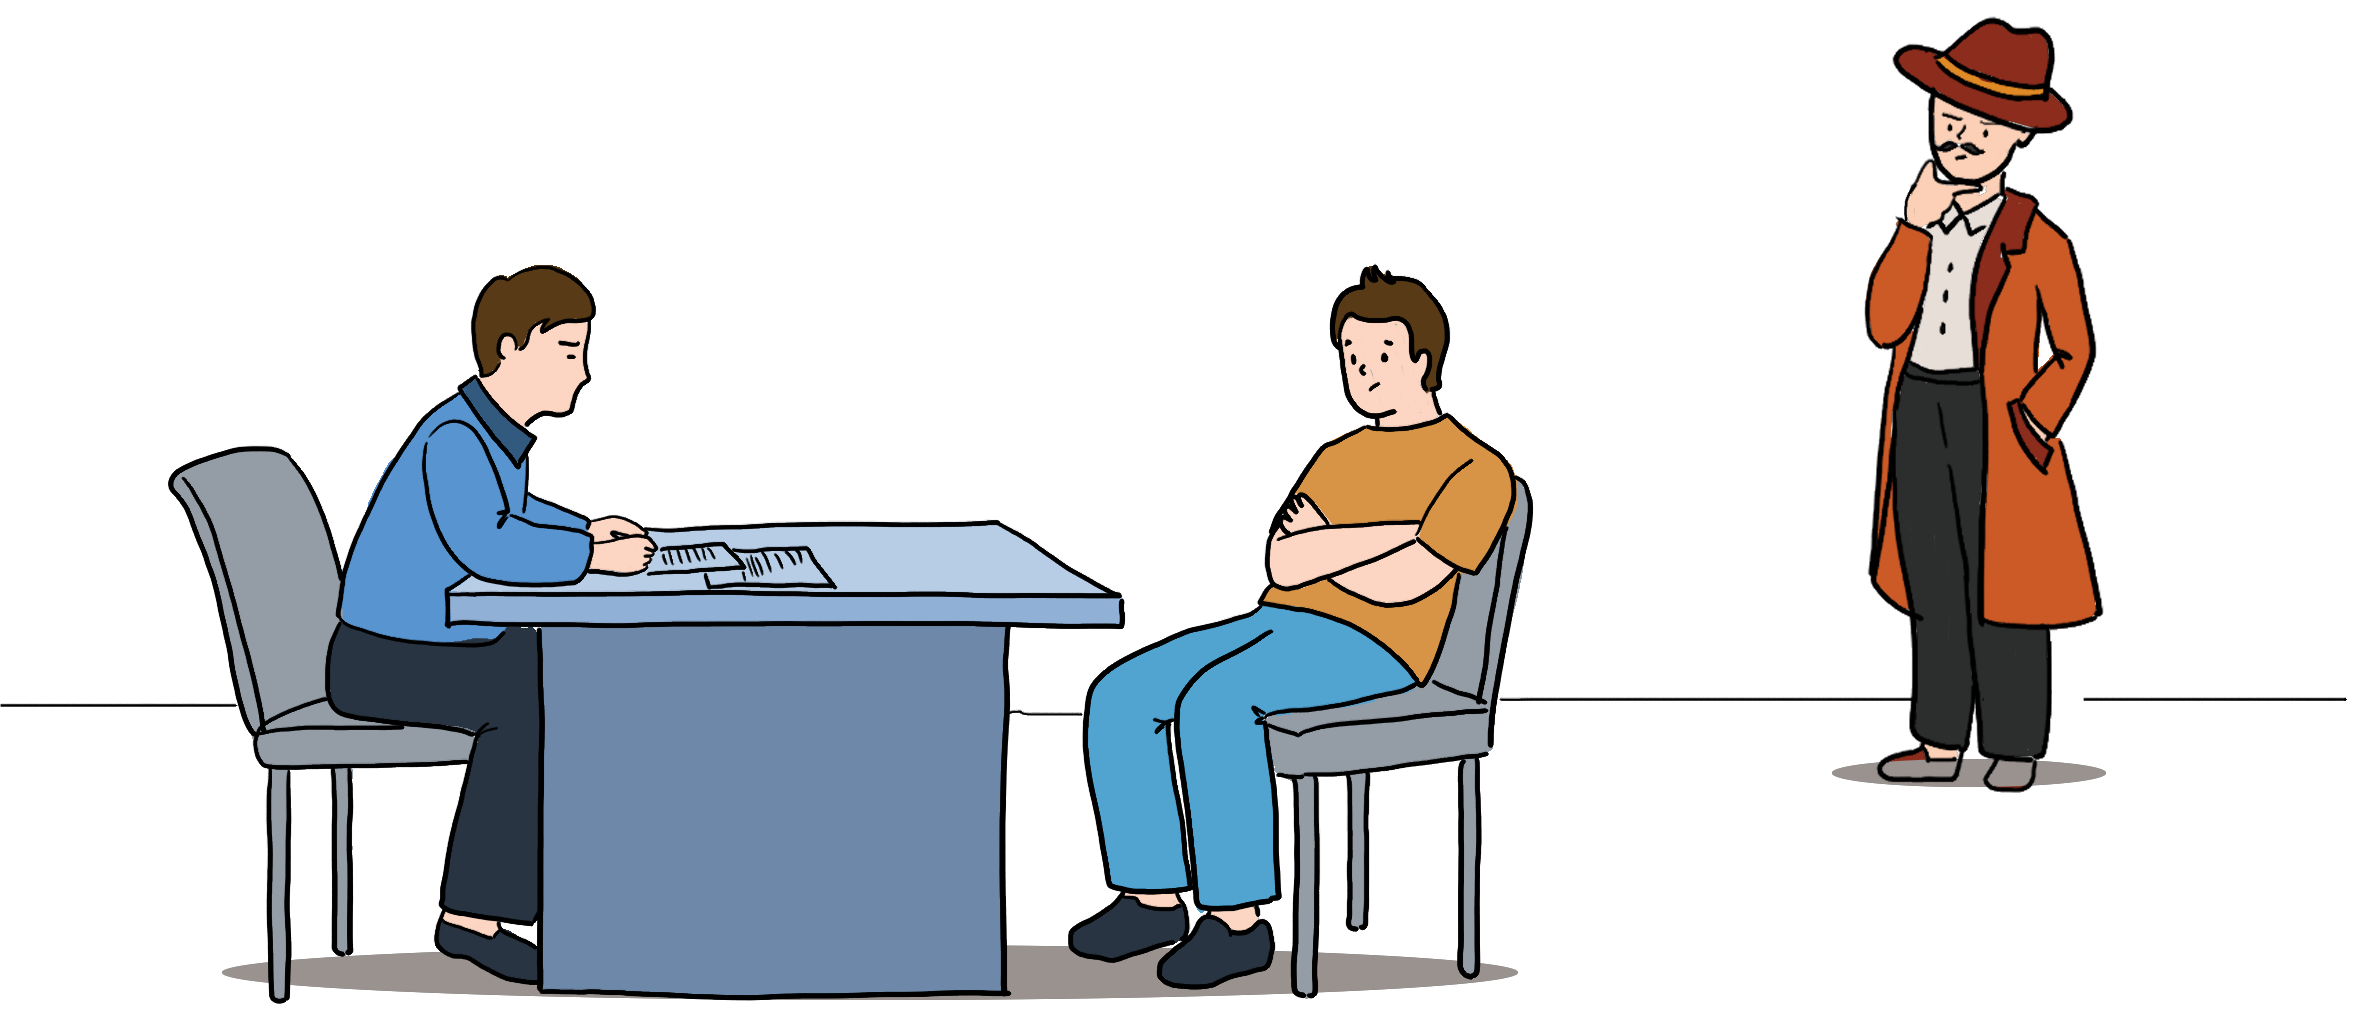
\includegraphics[width=0.85\linewidth]{xp}
	\vspace*{-10pt}
\end{figure}
\vspace*{-10pt}
{\color{toancuabi}\rule{1\linewidth}{0.1pt}}
\begingroup
\AddToShipoutPicture*{\put(115,315){
\includegraphics[scale=1]{../tieude11.pdf}}} 
\centering
\endgroup
\vspace*{45pt}

\begin{multicols}{2}
	$\pmb{1.}$ Ở nhà một mình, bé Hoa rót ra một cốc sữa đầy và uống hết một nửa. Sau đó Hoa rót thêm nước ép táo vào cho đầy cốc, rồi lại uống hết một nửa. Cuối cùng, bé lại rót thêm nước ép táo vào đầy cốc rồi uống hết sạch cả cốc. Hỏi bé Hoa đã uống thứ gì nhiều hơn: sữa hay nước ép táo?
	\begin{figure}[H]
		\centering
		\vspace*{-5pt}
		\captionsetup{labelformat= empty, justification=centering}
		
\includegraphics[width=0.9\linewidth]{Pi6_bai1}
		\vspace*{-5pt}
	\end{figure}
	$\pmb{2.}$ Dê con và Sói cùng thi xem ai chạy từ nhà tới bờ suối và quay ngược lại nhanh hơn. Biết rằng khoảng cách từ nhà tới bờ suối là $100$ bước nhảy của Dê con. Một bước nhảy của Sói dài gấp $3$ lần một bước nhảy của Dê con. Tuy nhiên trong khoảng thời gian Sói nhảy được một bước thì Dê con lại nhảy được $3$ bước. Hỏi ai sẽ chiến thắng?
	\begin{figure}[H]
		\centering
		\vspace*{-5pt}
		\captionsetup{labelformat= empty, justification=centering}
		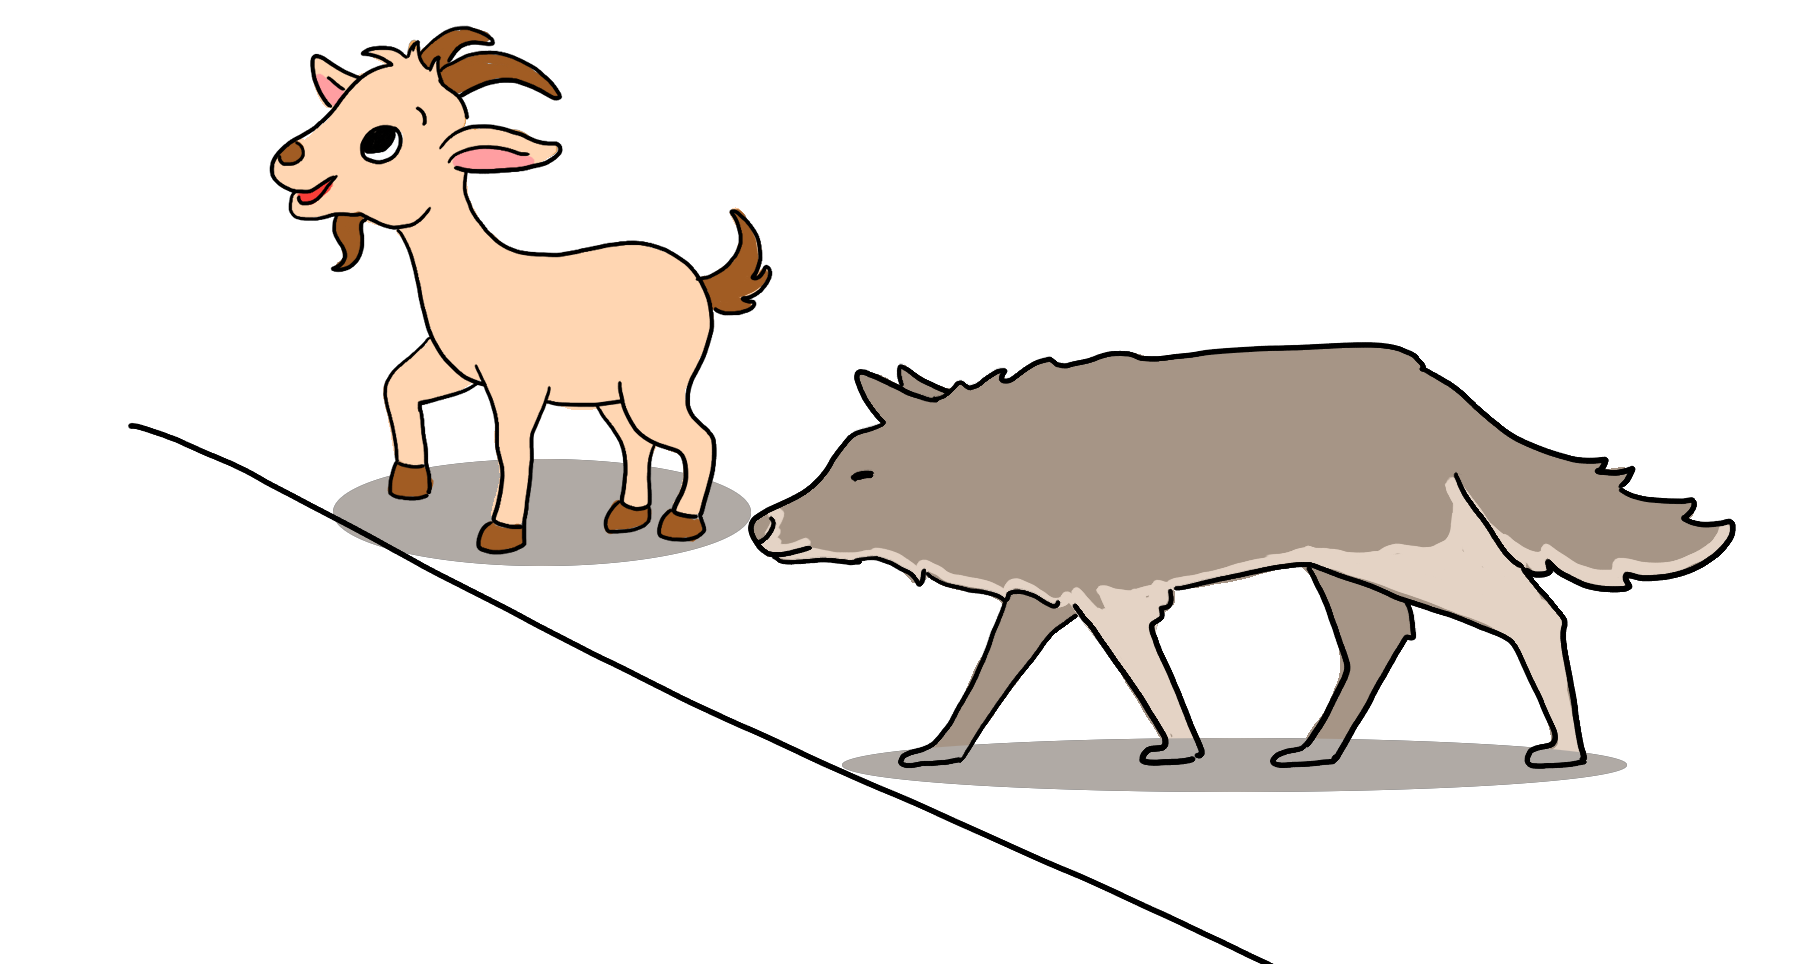
\includegraphics[width=0.95\linewidth]{Pi6_bai2}
		\vspace*{-5pt}
	\end{figure}
	$\pmb{3.}$ 	Có tất cả $25$ chú chim cúc cu và gà trống cùng tham gia một cuộc thi hùng biện giữa các loài vật. Trong số $15$ chú chim bất kỳ luôn có ít nhất một chú gà trống, và trong số $12$ chú chim bất kỳ luôn có ít nhất một chú chim cúc cu. Hỏi trong cuộc thi đó có bao nhiêu chú gà trống và bao nhiêu chú chim cúc cu tham gia?
	\begin{figure}[H]
		\centering
		\vspace*{-5pt}
		\captionsetup{labelformat= empty, justification=centering}
		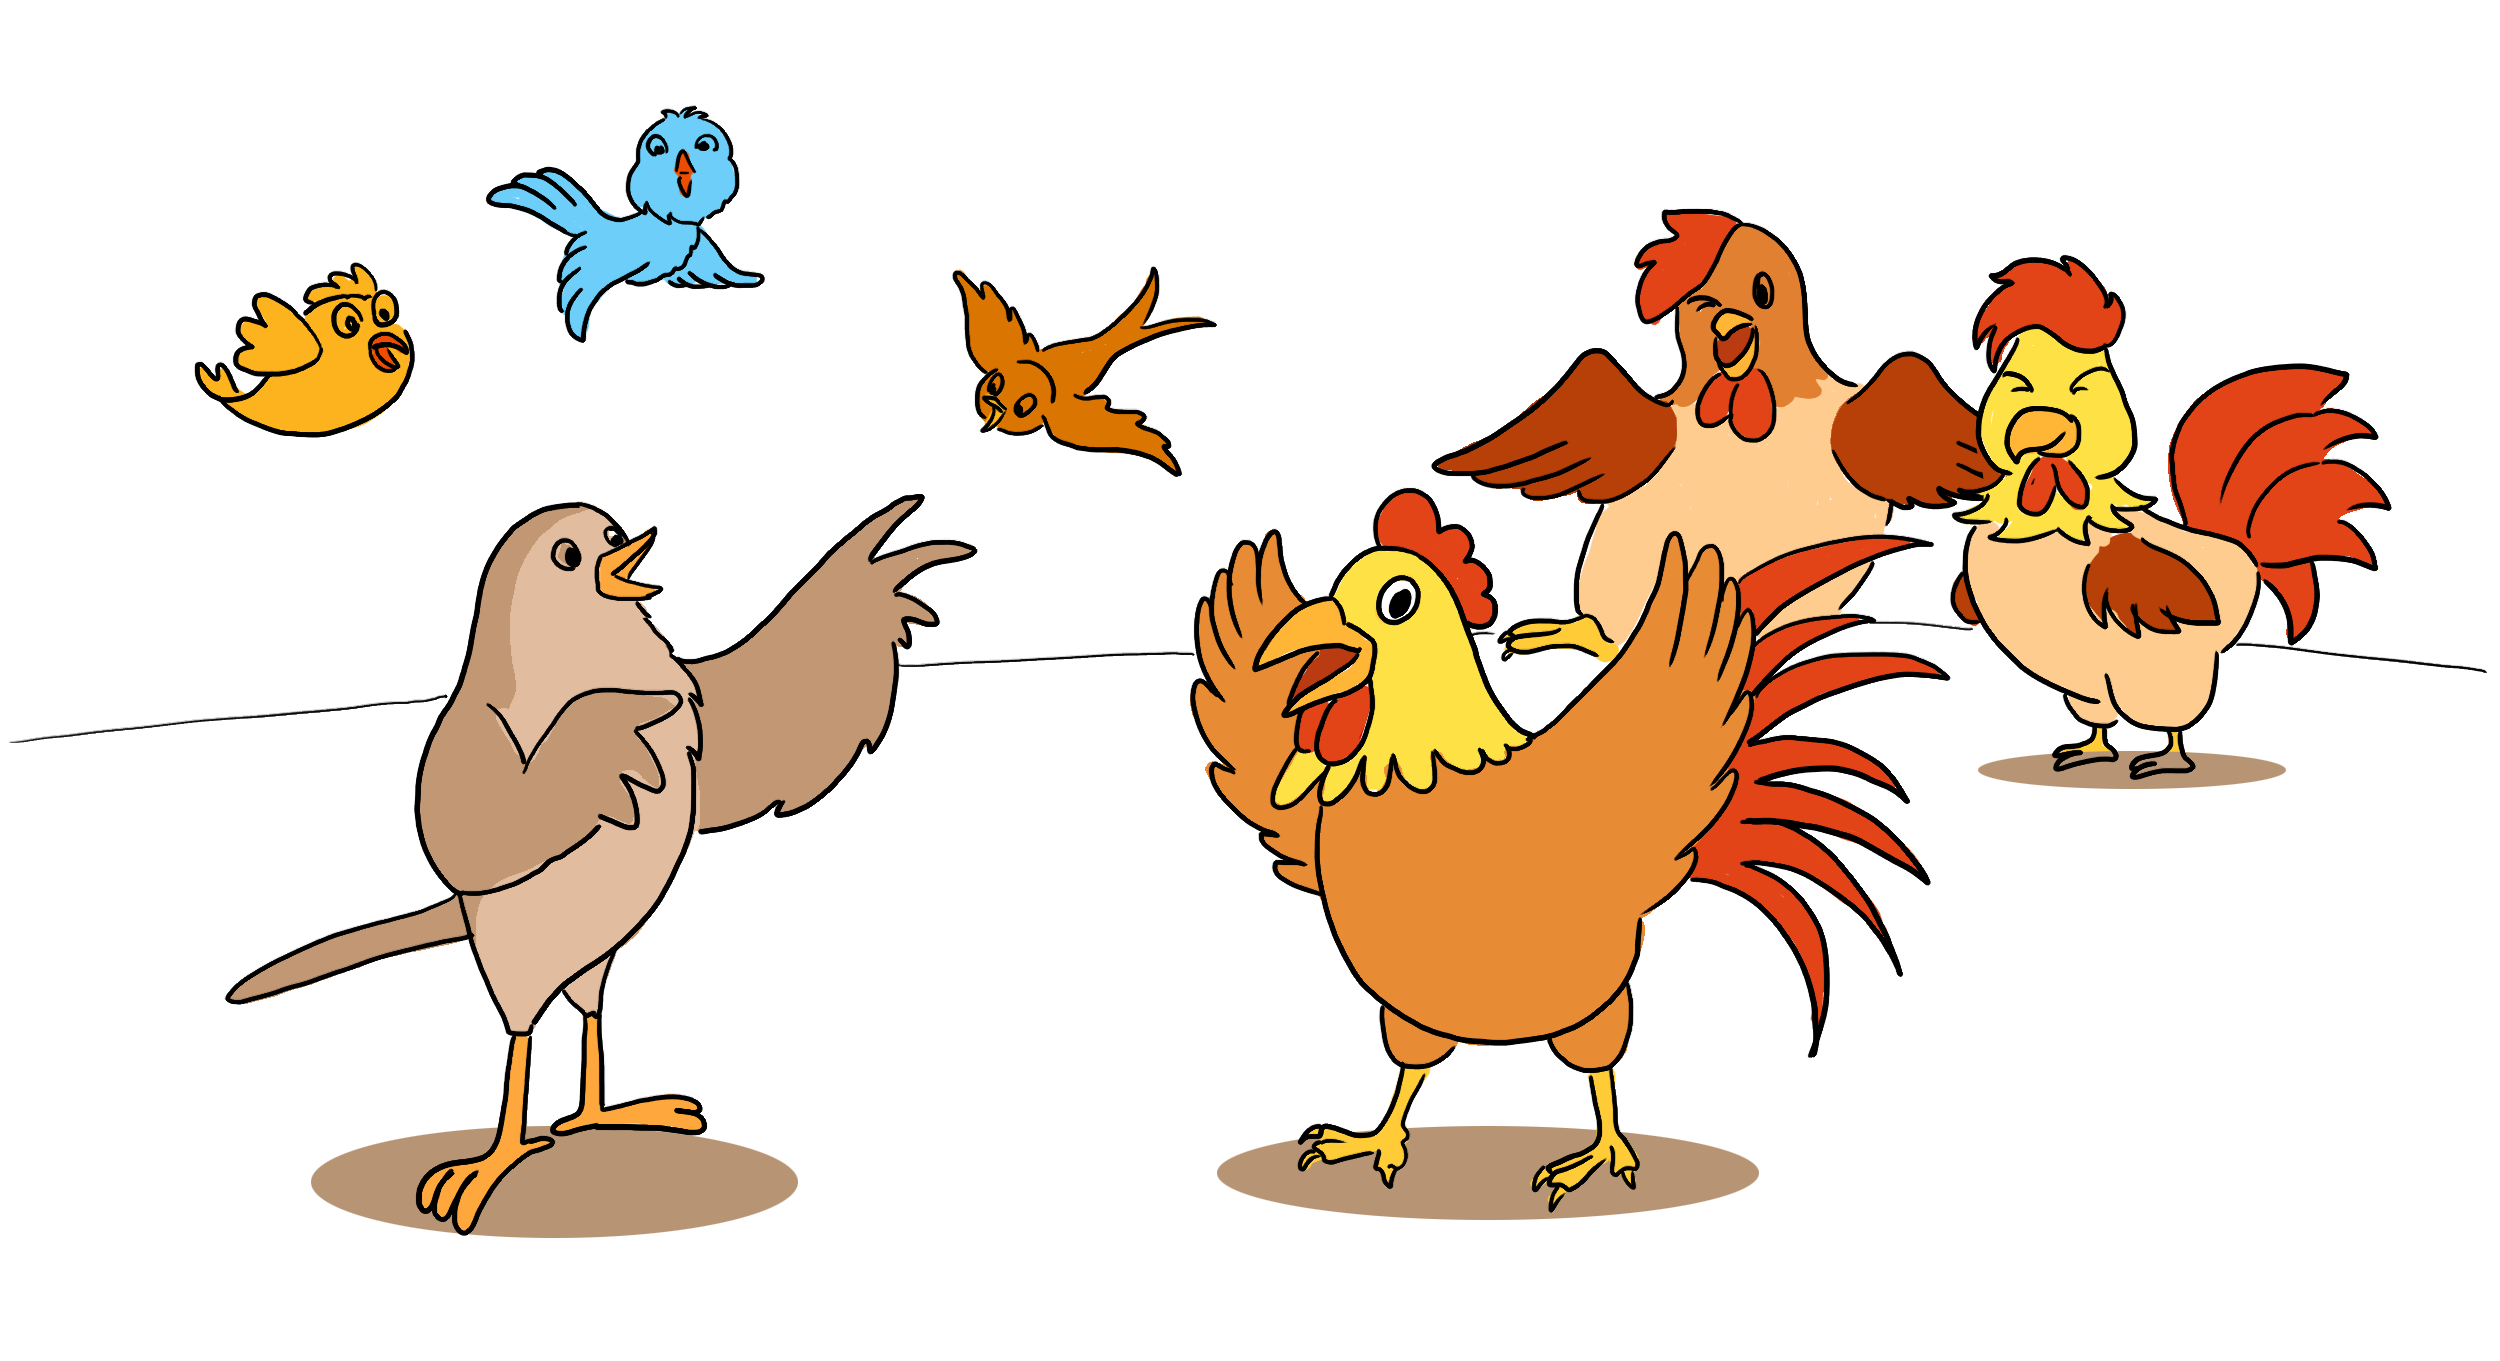
\includegraphics[width=1\linewidth]{Pi6_bai3}
		\vspace*{-10pt}
	\end{figure}
	$\pmb{4.}$ Người ta trồng trong công viên hai loài cây gồm phượng vĩ và sấu. Trong đó phượng vĩ chiếm $60\%$ tổng số hai loài. Vào mùa xuân cây sấu được trồng thêm trong công viên, do đó cây phượng vĩ chỉ còn chiếm $20\%$ tổng số cây. Sang mùa thu người ta lại trồng thêm  phượng vĩ, vì thế cây phượng vĩ lại chiếm $60\%$ tổng số cây hai loài. Hỏi sau hai lần trồng thì số cây trong công viên tăng lên bao nhiêu lần?
	\begin{figure}[H]
		\centering
		\vspace*{-5pt}
		\captionsetup{labelformat= empty, justification=centering}
		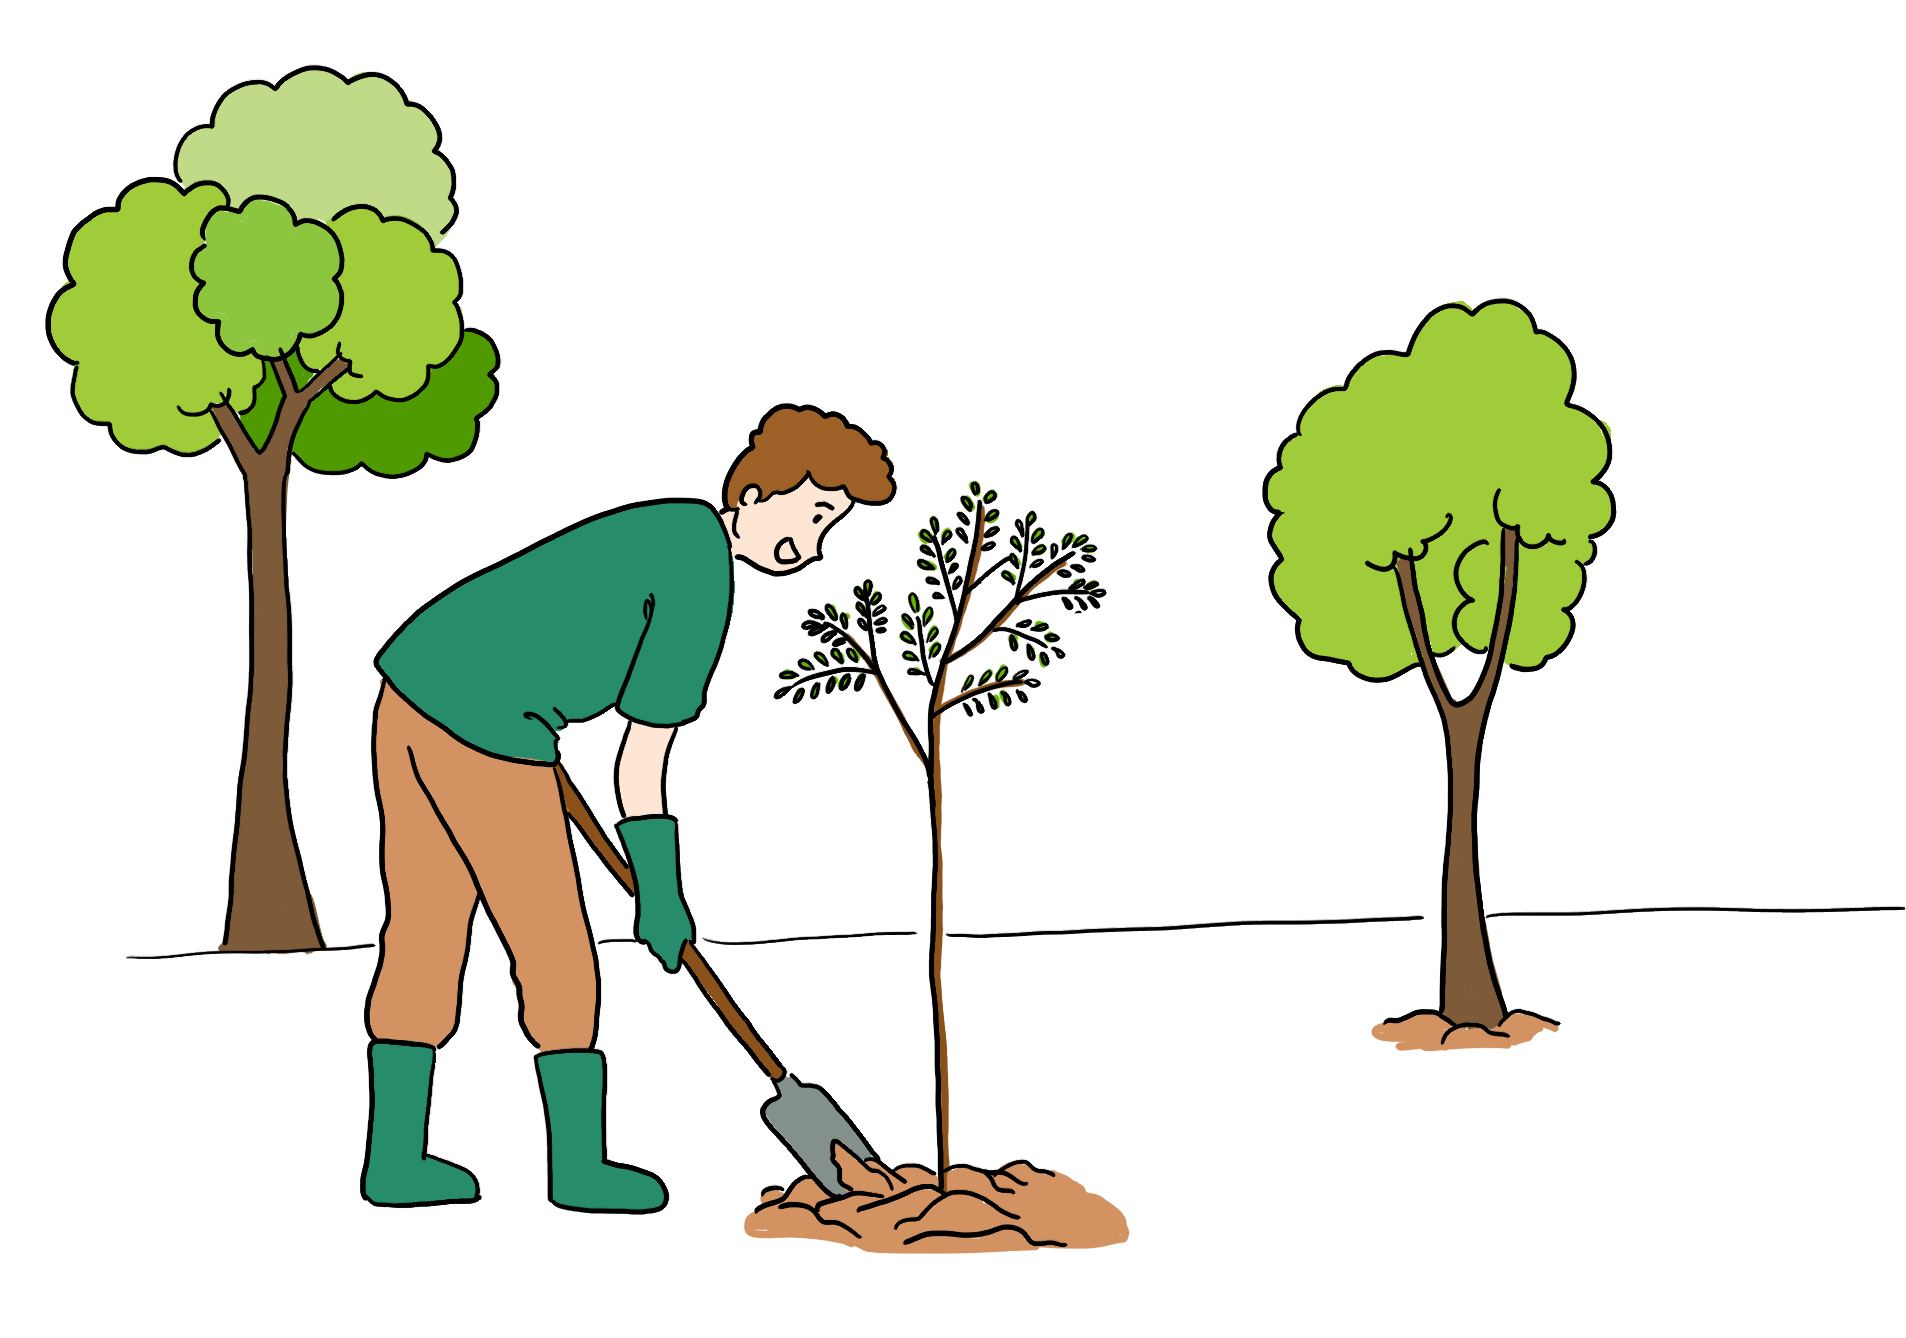
\includegraphics[width=1\linewidth]{Pi6_bai4}
		\vspace*{-10pt}
	\end{figure}
	$\pmb{5.}$ Alibaba đột nhập vào một hang động, trong đó có $100$ chiếc bao vải đựng đầy những đồng tiền. Một chiếc bao vải trong số đó chỉ đựng toàn đồng tiền giả. Khối lượng của một đồng tiền thật là $10$ gram, trong khi khối lượng của một đồng tiền giả là $9$ gram. Hỏi Alibaba làm thế nào để chỉ cân một lần duy nhất (bằng một cái cân chính xác có hiển thị số) tìm ra được bao vải chứa các đồng tiền giả?
	\begin{figure}[H]
		\centering
		\vspace*{-5pt}
		\captionsetup{labelformat= empty, justification=centering}
		
\includegraphics[width=1\linewidth]{Pi6_bai5}
		\vspace*{-10pt}
	\end{figure}
	$\pmb{6.}$ 	Trên một bàn cờ $8\times8$ người ta xếp một số lớn nhất có thể các quân Tượng sao cho không có hai quân Tượng nào ``ăn" lẫn nhau. Em hãy chứng minh rằng số các cách xếp khác nhau như vậy là một số chính phương (tức là bình phương của một số tự nhiên).
	\begin{figure}[H]
		\centering
		\vspace*{-5pt}
		\captionsetup{labelformat= empty, justification=centering}
		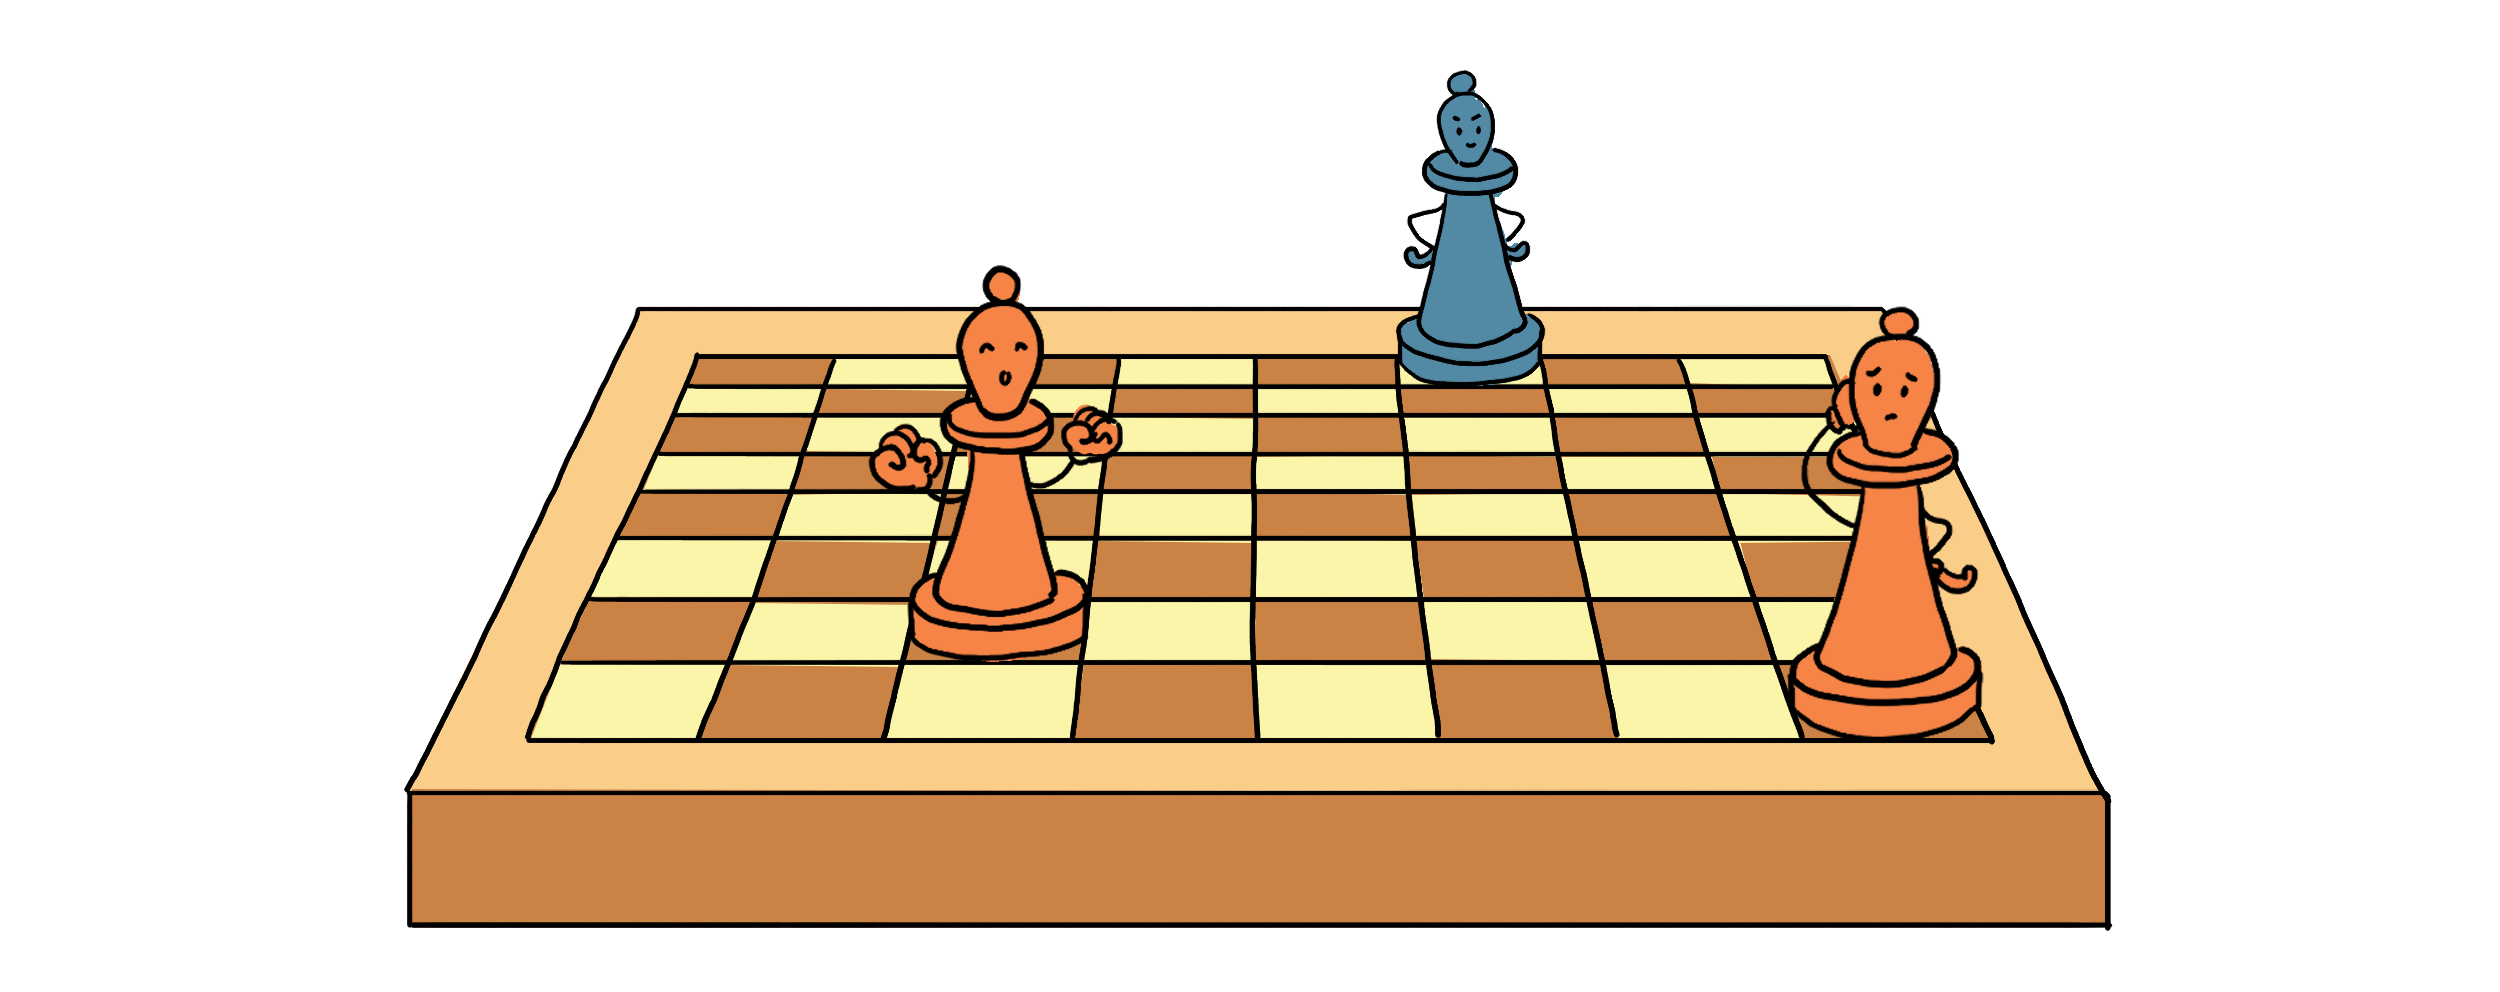
\includegraphics[width=1\linewidth]{Pi6_bai6}
		\vspace*{-5pt}
	\end{figure}
\end{multicols}
\newpage
\begingroup
\AddToShipoutPicture*{\put(112,645){
\includegraphics[scale=1]{../tieude2.pdf}}} 
\centering
\endgroup
\vspace*{55pt}

\begin{multicols}{2}
	$\pmb{1.}$	Bạn Công đã trả $24$ nghìn đồng để mua được $1$ cuốn vở, $2$ chiếc bút chì và $1$ cái tẩy. Bạn Nam thì trả tận $54$ nghìn đồng để mua được $2$ cuốn vở, $3$ chiếc bút chì và $3$ cái tẩy. Hỏi bạn An đã trả bao nhiêu tiền để mua được $2$ cuốn vở, $5$ chiếc bút chì và $1$ cái tẩy?
	\begin{figure}[H]
		\centering
		\vspace*{-5pt}
		\captionsetup{labelformat= empty, justification=centering}
		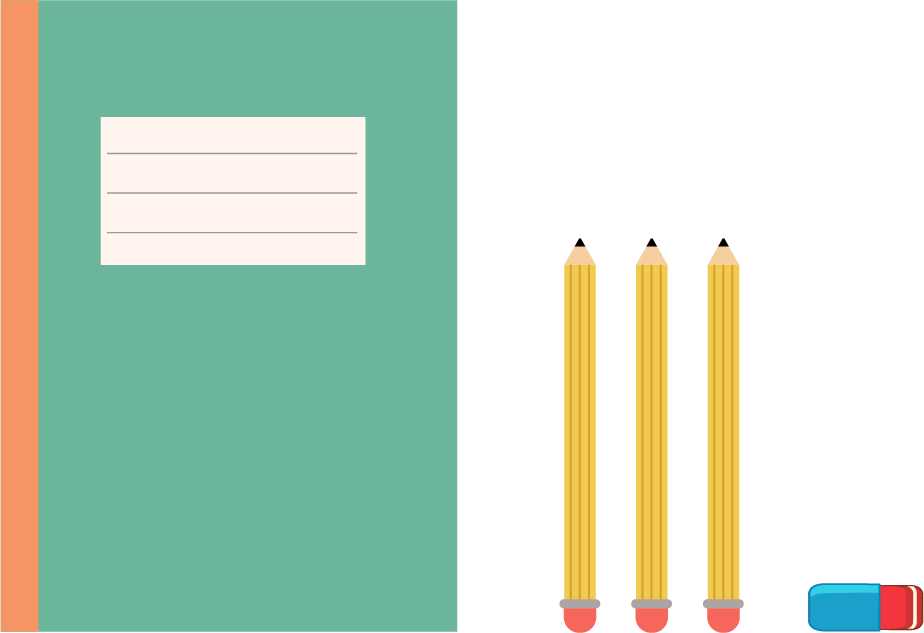
\includegraphics[width=1\linewidth]{Pi3_bai1}
		\vspace*{-10pt}
	\end{figure}
	\textit{Lời giải.} 	Cả $3$ bạn Công, Nam và An đã mua $5$ cuốn vở, $10$ chiếc bút chì và $5$ cái tẩy, bằng đúng $5$ lần số lượng mà Công đã mua. Vì thế $3$ bạn đã trả số tiền là 
	\begin{align*}
		24\times 5=120 \text{(nghìn đồng).} 
	\end{align*}
	Công và Nam đã trả $78$ nghìn đồng. Suy ra An đã trả 
	\begin{align*}
		120-78 = 42 \text{(nghìn đồng).}	
	\end{align*}
	 $\pmb{2.}$ Bác Tuyết mang sữa đựng đầy trong hai chiếc thùng ra chợ bán. Lượng sữa trong thùng to nhiều gấp $3$ lần lượng sữa trong chiếc thùng nhỏ. Khi trong chiếc thùng nhỏ còn có $15$ lít sữa, còn thùng to còn $35$ lít sữa, bác Tuyết đổ dồn một lượng sữa từ thùng to cho đầy chiếc thùng nhỏ. Khi đó trong chiếc thùng to lượng sữa còn lại  đầy tới một nửa thùng. Hỏi bác Tuyết đã đổ bao nhiêu sữa từ thùng to sang thùng nhỏ, và dung tích của mỗi thùng là bao nhiêu?
	 \begin{figure}[H]
	 	\centering
	 	\vspace*{5pt}
	 	\captionsetup{labelformat= empty, justification=centering}
	 	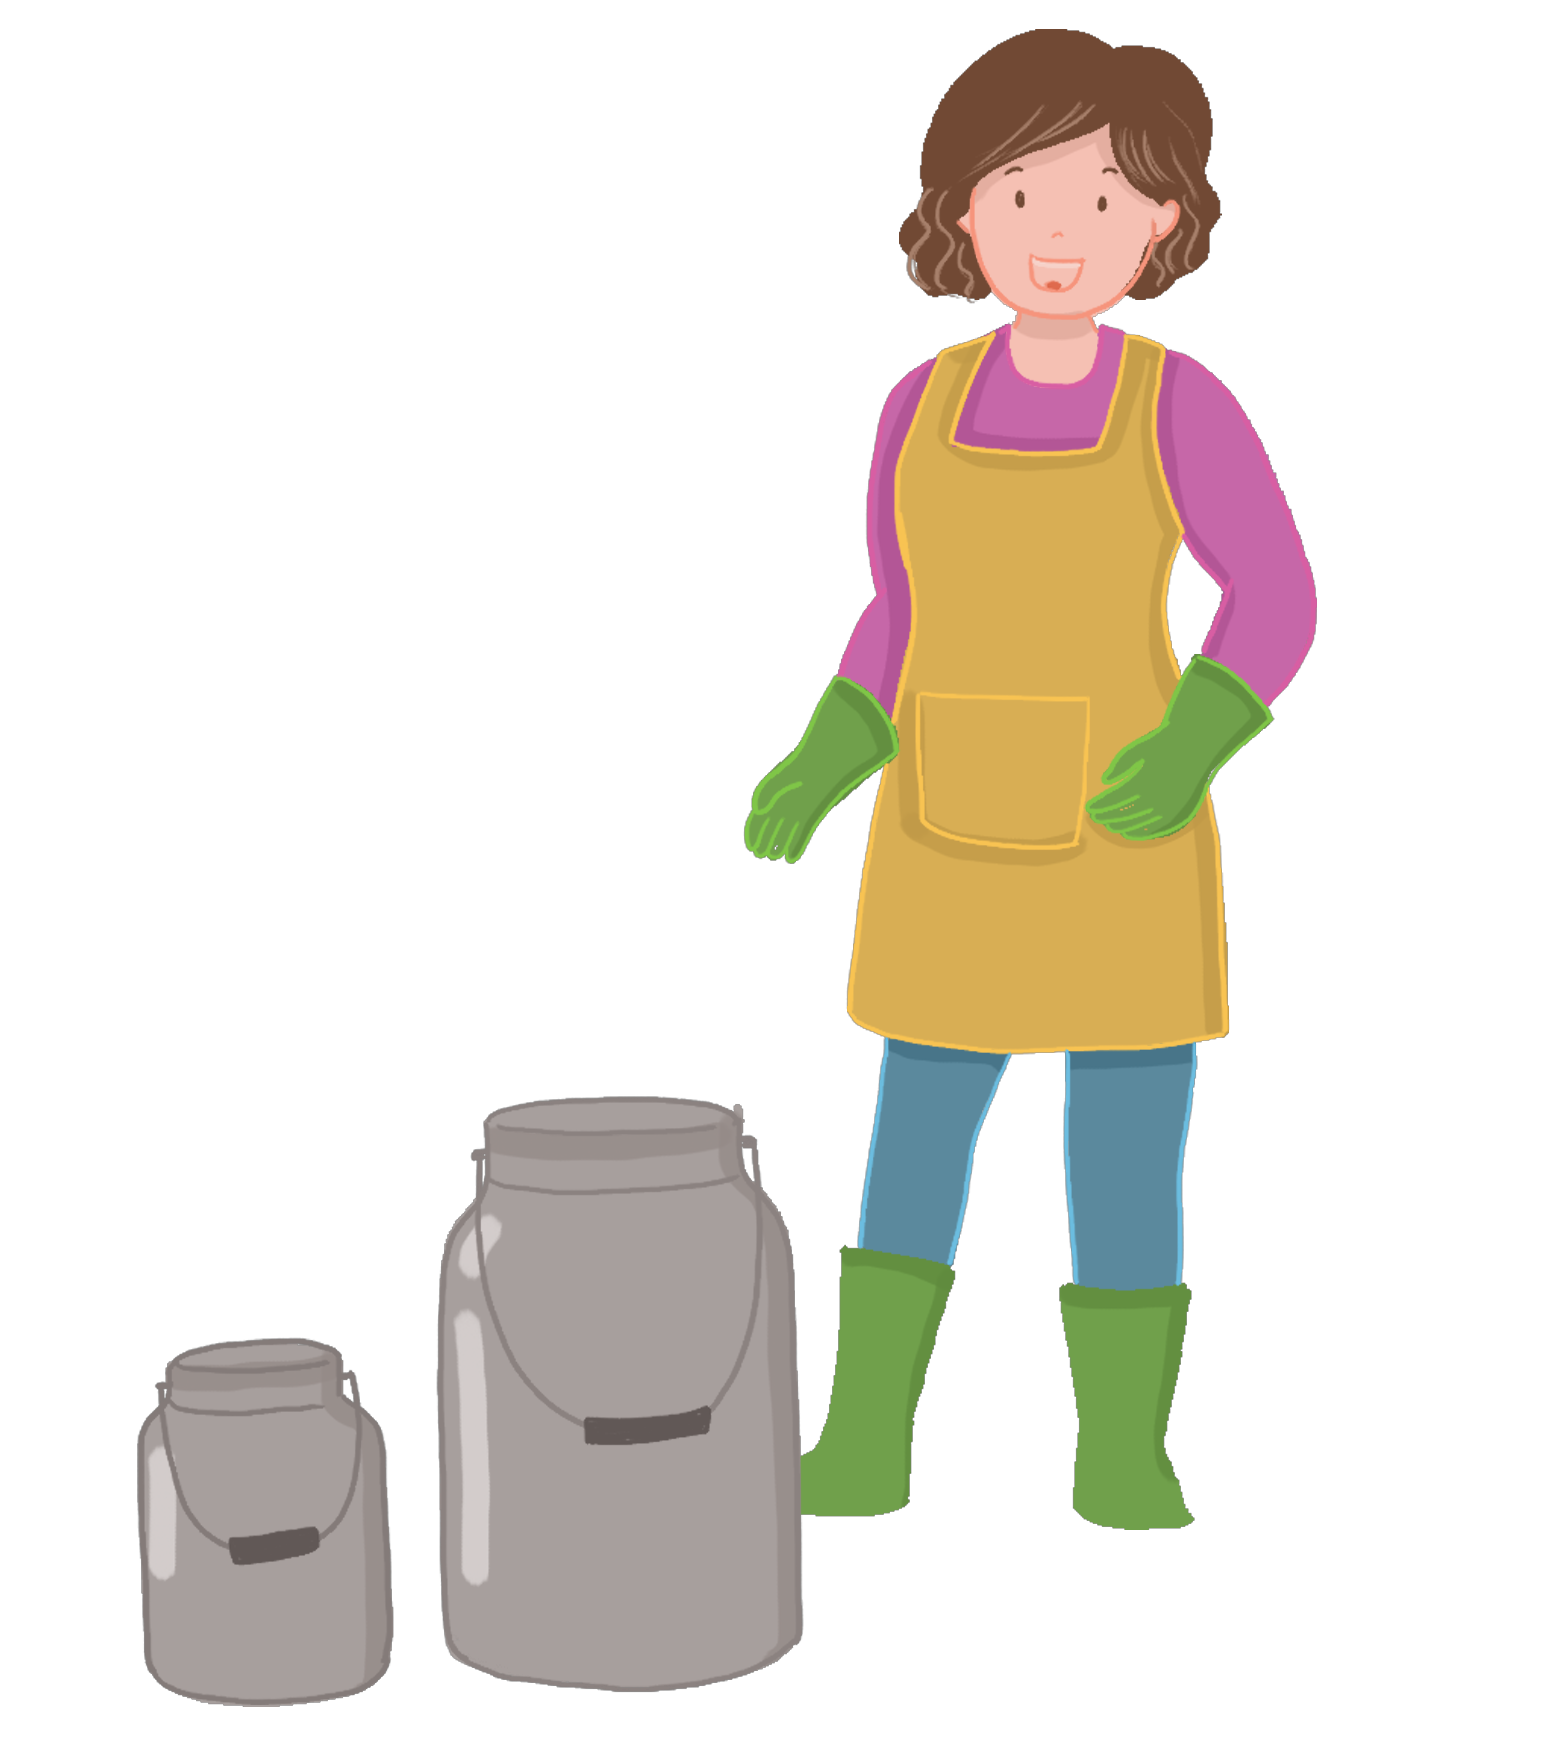
\includegraphics[width=0.75\linewidth]{Pi3_bai2}
	 	\vspace*{-5pt}
	 \end{figure}
	\textit{Lời giải}. Các em nhận thấy, sau khi đổ dồn sữa, số sữa còn lại trong thùng to sẽ gấp rưỡi số sữa trong thùng nhỏ. Gọi số sữa đã đổ dồn sang thùng nhỏ là $a$ ( lít) thì ta có 
	\begin{align*}
		1{.}5\times (15+a)=35-a.
	\end{align*}
	Từ đây suy ra $a =5$. Do đó dung tích của thùng bé là $20$ lít và thùng to là $60$ lít.
	\vskip 0.1cm
	Cách giải khác. Lượng sữa bác Tuyết có lúc đổ từ thùng to thùng nhỏ là $50$ và bằng $2{.}5$ lần dung tích thùng nhỏ. Vậy dung tích thùng nhỏ là 
	\begin{align*}
		50: 2{.}5  = 20 \text{(lít).} 
	\end{align*}
	Số sữa được đổ từ thùng to sang thùng nhỏ là: 
	\begin{align*}
		25-20=5 \text{(lít).} 
	\end{align*}
	Và dung tích thùng to là 
	\begin{align*}
		3 \times 20=60 \text{(lít).}
	\end{align*}
	$\pmb{3.}$ Một tấn hoa quả được chở tới siêu thị: táo được đóng theo các thùng gỗ  $48$ kg/thùng, lê được đóng trong các thùng gỗ $20$ kg/thùng, mận đựng trong hộp giấy theo $14$ kg/hộp còn nho đựng trong các hộp giấy theo $10$ kg/hộp. Biết rằng số kg táo được chở tới nhiều gấp đôi số kg lê, còn số kg mận và nho là bằng nhau, hỏi số lượng mỗi loại hoa quả đã được vận chuyển tới cửa hàng là bao nhiêu?
	\begin{figure}[H]
		\centering
		\vspace*{-5pt}
		\captionsetup{labelformat= empty, justification=centering}
		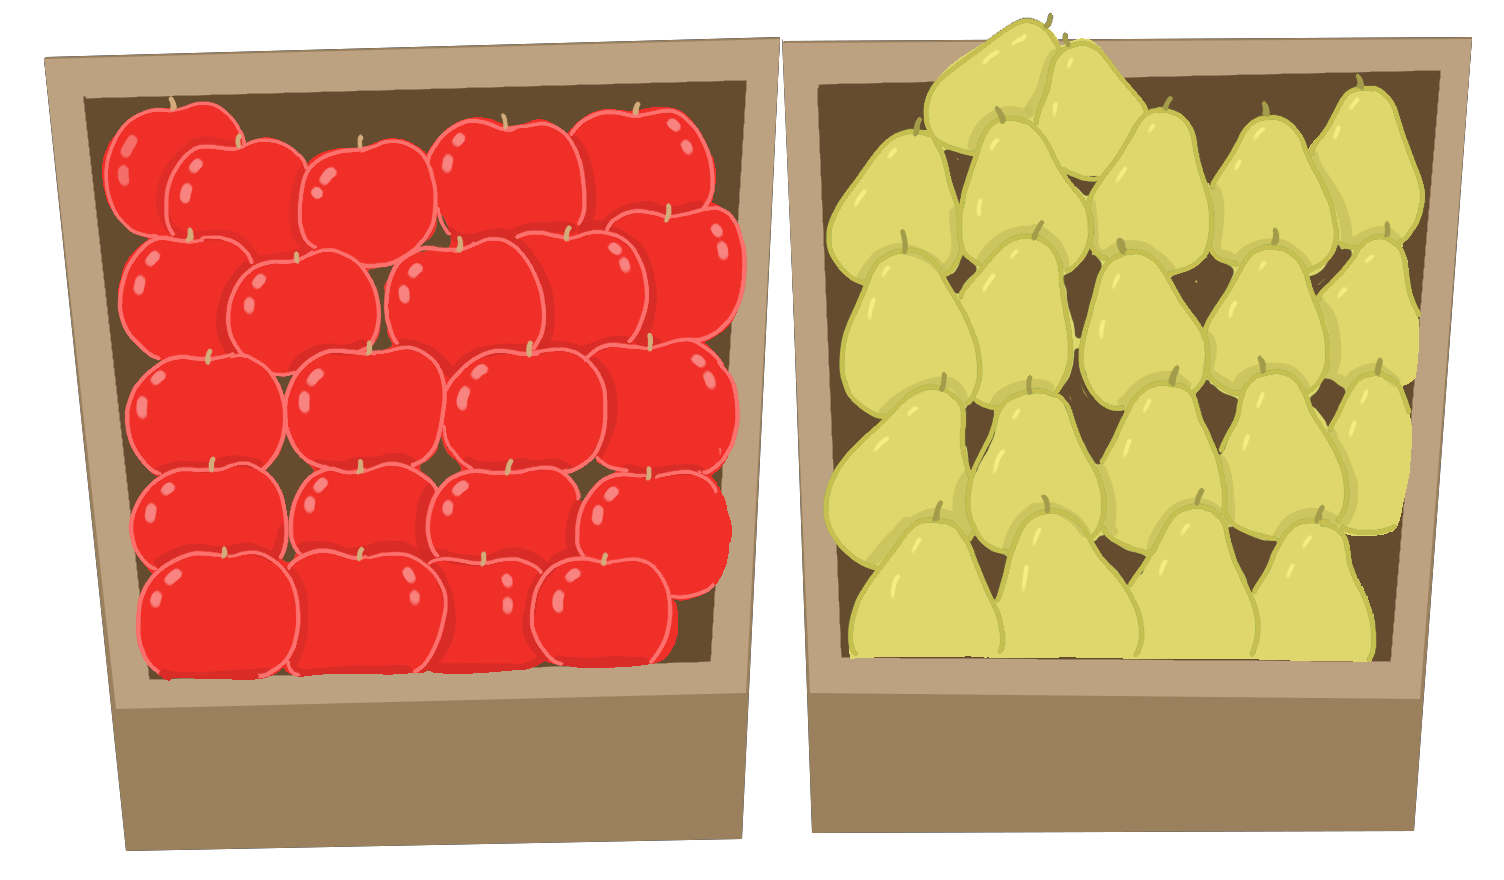
\includegraphics[width=1\linewidth]{Pi3_bai3}
		\vspace*{-15pt}
	\end{figure}
	\textit{Lời giải.} Gọi số thùng táo là $a$, số hộp mận là $b$. Suy ra số thùng lê là 
	\begin{align*}
		\dfrac{48 \times a}{40} = \dfrac{6 \times a}{5}.
	\end{align*}
	Số hộp nho là
	\begin{align*}
		\dfrac{14 \times b}{10} = \dfrac{7 \times b}{5}.
	\end{align*}
	Theo đề bài ta có tổng số kg các loại quả là: 
	\begin{align*}
		48a+24a+14b+14b =1000. 
	\end{align*}
	Có nghĩa là
	\begin{align*}
		72a+28b=1000.
	\end{align*}
	Chia cả hai vế cho $4$, ta nhận được 
	\begin{align*}
		18a+7b=250.
	\end{align*}
	Vì $\dfrac{6 \times a}{5}$ là số nguyên, suy ra $a$ chia hết cho $5$. Tương tự $b$ chia hết cho $5$. Đặt $a = 5m,b=5n$ (trong đó $m$, $n$ là các số nguyên dương),  ta rút ra được hệ thức
	\begin{align*}
		18m+7n = 50.
	\end{align*}
	Từ đây suy ra $1\le m \le 2$.
	\vskip 0.1cm 
	Thử trực tiếp, với $m=1$ suy ra $7n=32$ (loại, do $n$ là số nguyên). 
	\vskip 0.1cm
	Với $m=2$ suy ra $n=2$. Vậy $a=10,b=10$.
	\vskip 0.1cm 
	Đáp số: $10$ thùng táo, $12$ thùng lê, $14$ hộp nho và $10$ hộp mận.
	\vskip 0.1cm
	$\pmb{4.}$ Bạn An khởi hành đi bộ từ làng $A$ tới làng $B$ lúc $8$h sáng. Đồng thời vào lúc đó, bạn Bình cũng đi bộ từ làng $B$ tới làng $A$. Hai bạn đều đi với vận tốc không đổi, nhưng có thể không bằng nhau. Khi gặp nhau ở giữa đường, bạn An còn phải đi thêm $32$ phút nữa, còn Bình phải đi thêm $18$ phút nữa thì mới tới nơi. Hỏi hai bạn đã gặp nhau sau bao lâu tính từ lúc khởi hành?
	\begin{figure}[H]
		\centering
		\vspace*{-5pt}
		\captionsetup{labelformat= empty, justification=centering}
		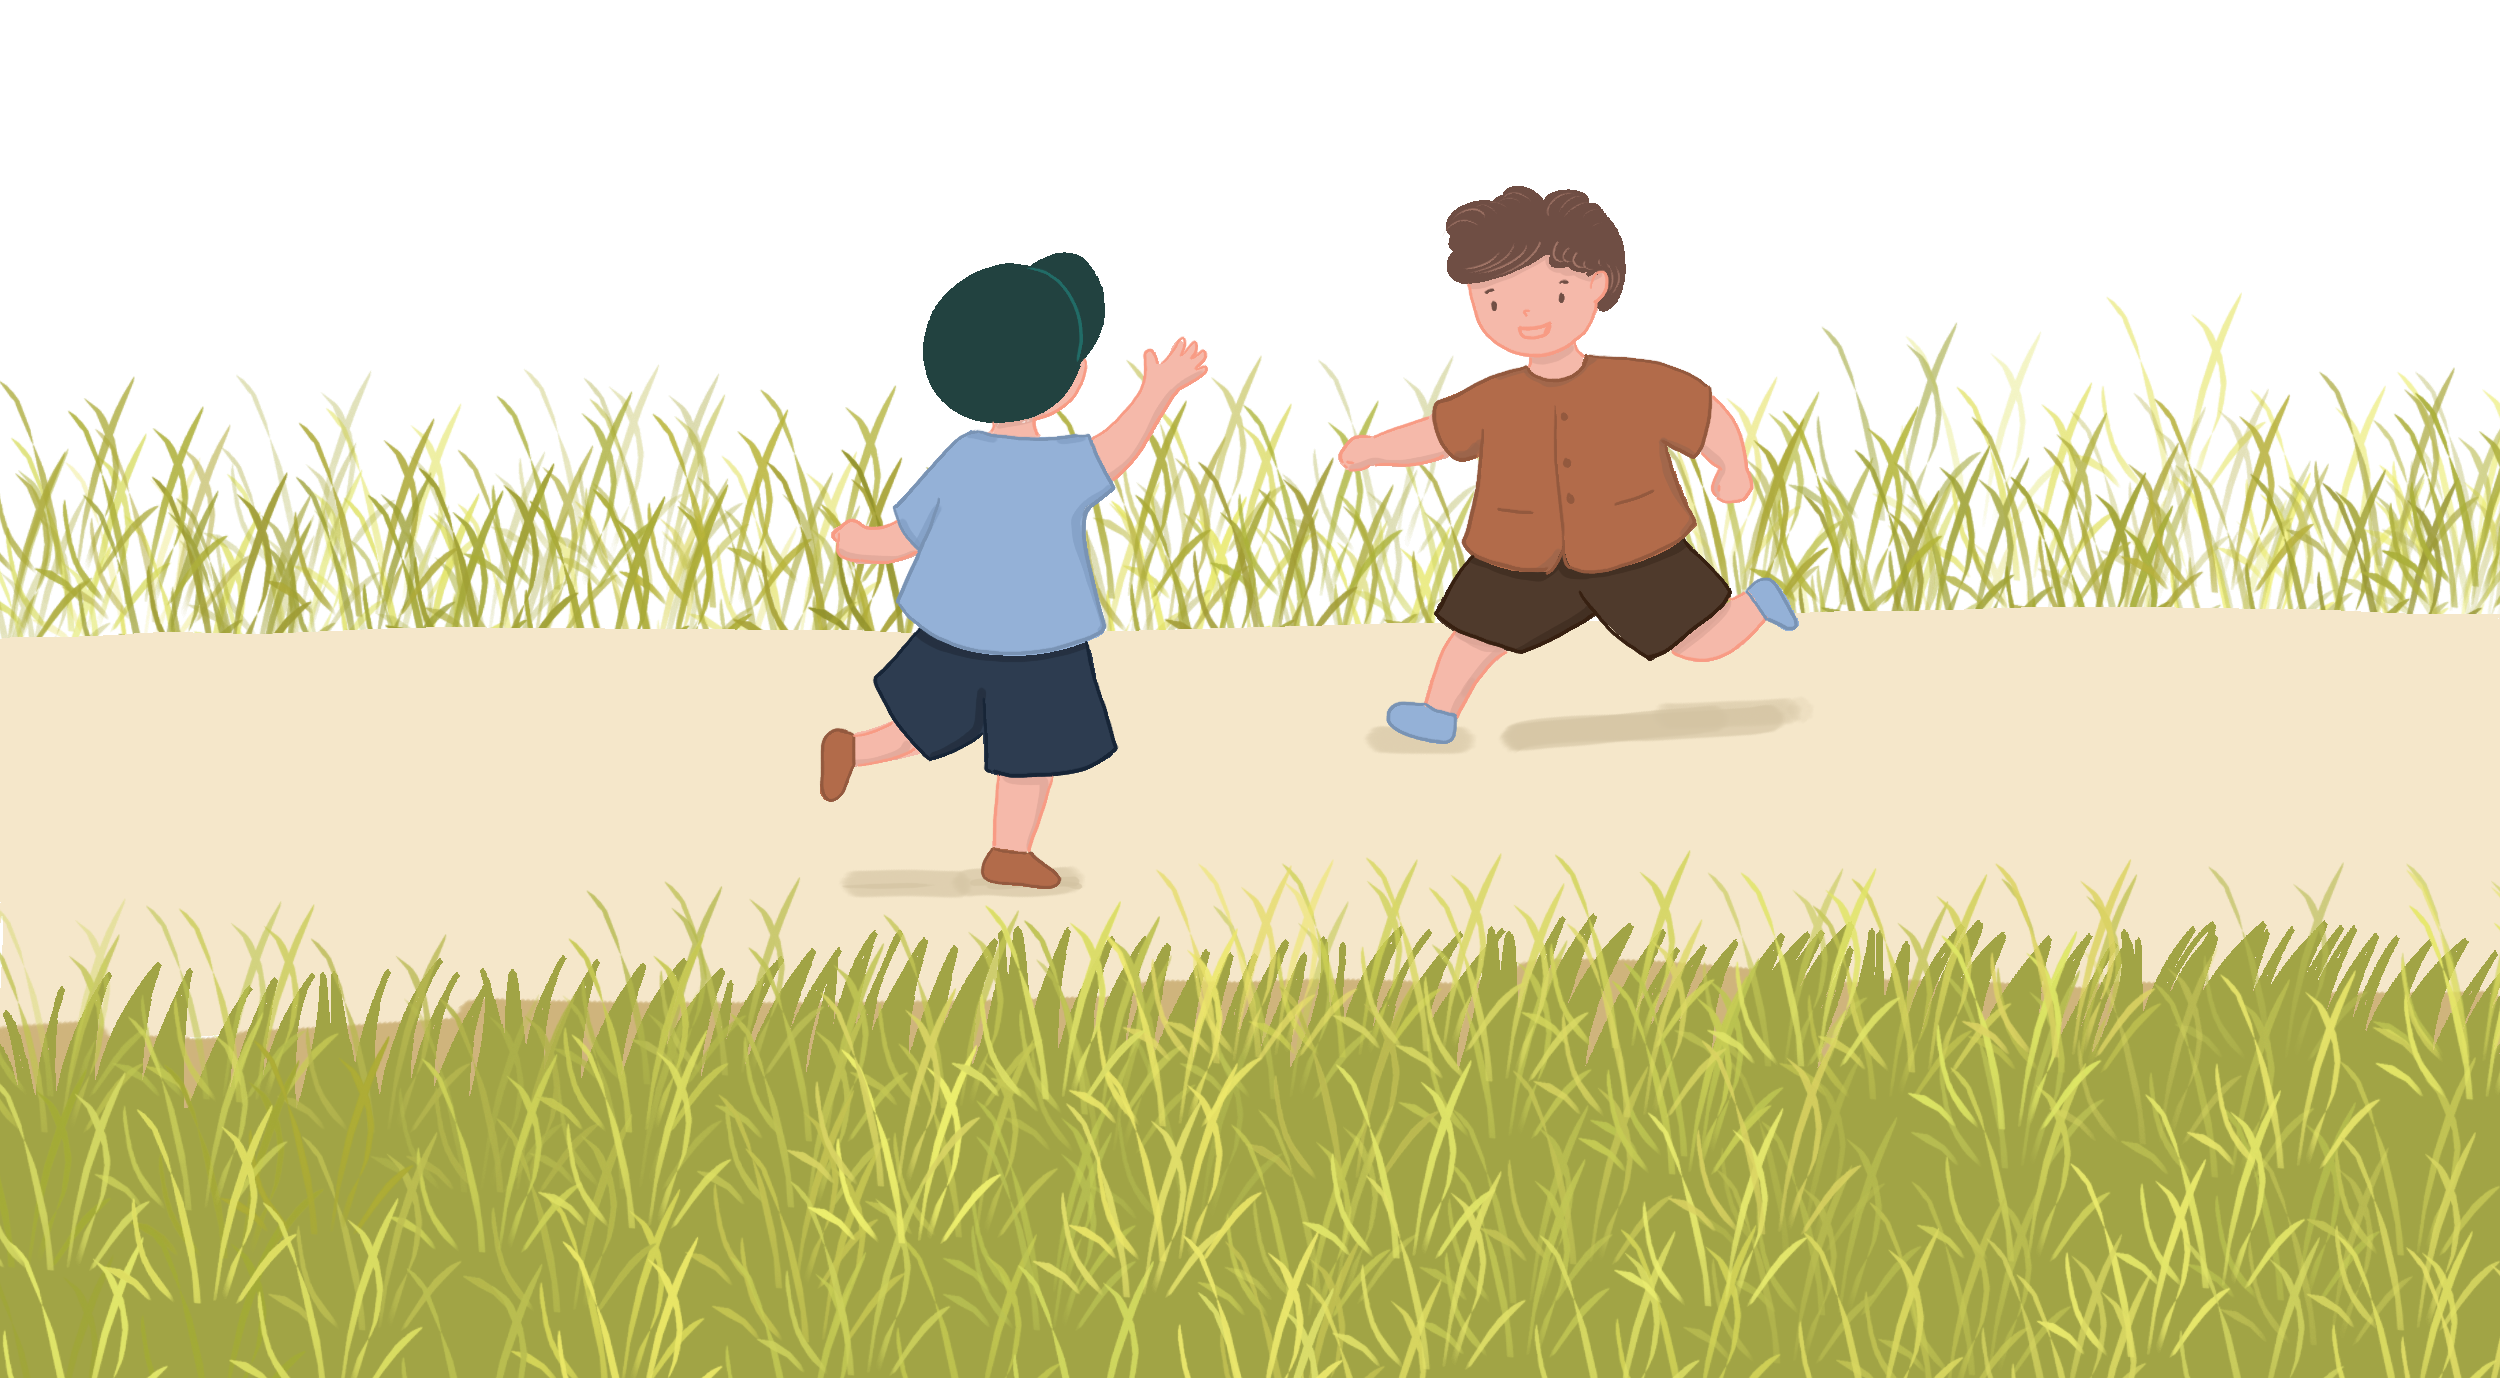
\includegraphics[width=1\linewidth]{Pi3_bai4}
		\vspace*{-15pt}
	\end{figure}
	\textit{Lời giải.} Gọi $a$ (m/phút) là vận tốc của An, còn $b$ (m/phút) là vận tốc của Bình. Giả sử sau khoảng thời gian là $t$ (phút) tính từ lúc khởi hành hai bạn đã gặp nhau. Suy ra
	\begin{align*}
		32a = tb
	\end{align*} 
	và
	\begin{align*}
		18b = ta. 
	\end{align*}
	Nhân hai vế các đẳng thức này với nhau và rút gọn cho $ab$ ta có
	\begin{align*}
		t^2=574.
	\end{align*}
	Từ đó suy ra $t=24$.
	Vậy các bạn đã gặp gỡ nhau sau $12$ phút tính từ lúc khởi hành.
	\vskip 0.1cm
	Cách khác:  Kí hiệu $C$ là điểm hai bạn gặp nhau, do quãng đường tỷ lệ thuận với thời gian đi của mỗi bạn nên tỷ số quãng đường $AC$ và $CB$ là
	$t:18$ đồng thời cũng là $32:t$.
	\begin{figure}[H]
		\vspace*{-5pt}
		\centering
		\captionsetup{labelformat= empty, justification=centering}
		\begin{tikzpicture}[toancuabi,scale=0.85]
			\draw (0,0) -- (8,0);
			\draw (0,0.2) node [above] {$A$};
			\draw (5,0.2) node [above] {$B$};
			\draw (8,0.2) node [above] {$C$};
			\draw [fill=white] (0,0) circle (3.5pt);
			\draw [fill=white] (5,0) circle (3.5pt);
			\draw [fill=white] (8,0) circle (3.5pt);
		\end{tikzpicture}
		\vspace*{-10pt}
	\end{figure}
	Suy ra $t=24$.
	Vậy các bạn đã gặp gỡ nhau sau $12$ phút tính từ lúc khởi hành.
	\vskip 0.1cm
	$\pmb{5.}$ Trong một cuộc thi thể thao do nhà vua Pháp tổ chức, $3$ chàng ngự lâm pháo thủ là Athos, Porthos và Aramis cùng D'Artagnan chia nhau bốn vị trí đầu tiên: $1$, $2$, $3$, $4$ (ứng với giải thưởng: nhất, nhì, ba, bốn). Tổng ba số chỉ vị trí mà Athos, Porthos và D'Artagnan giữ là bằng $6$. Tổng hai số chỉ vị trí mà Porthos và Aramis giữ cũng bằng $6$. Hỏi mỗi chàng ngự lâm đã chiếm các giải nào, biết Porthos chiếm được giải cao hơn Arthos?
	\begin{figure}[H]
		\centering
		\vspace*{-5pt}
		\captionsetup{labelformat= empty, justification=centering}
		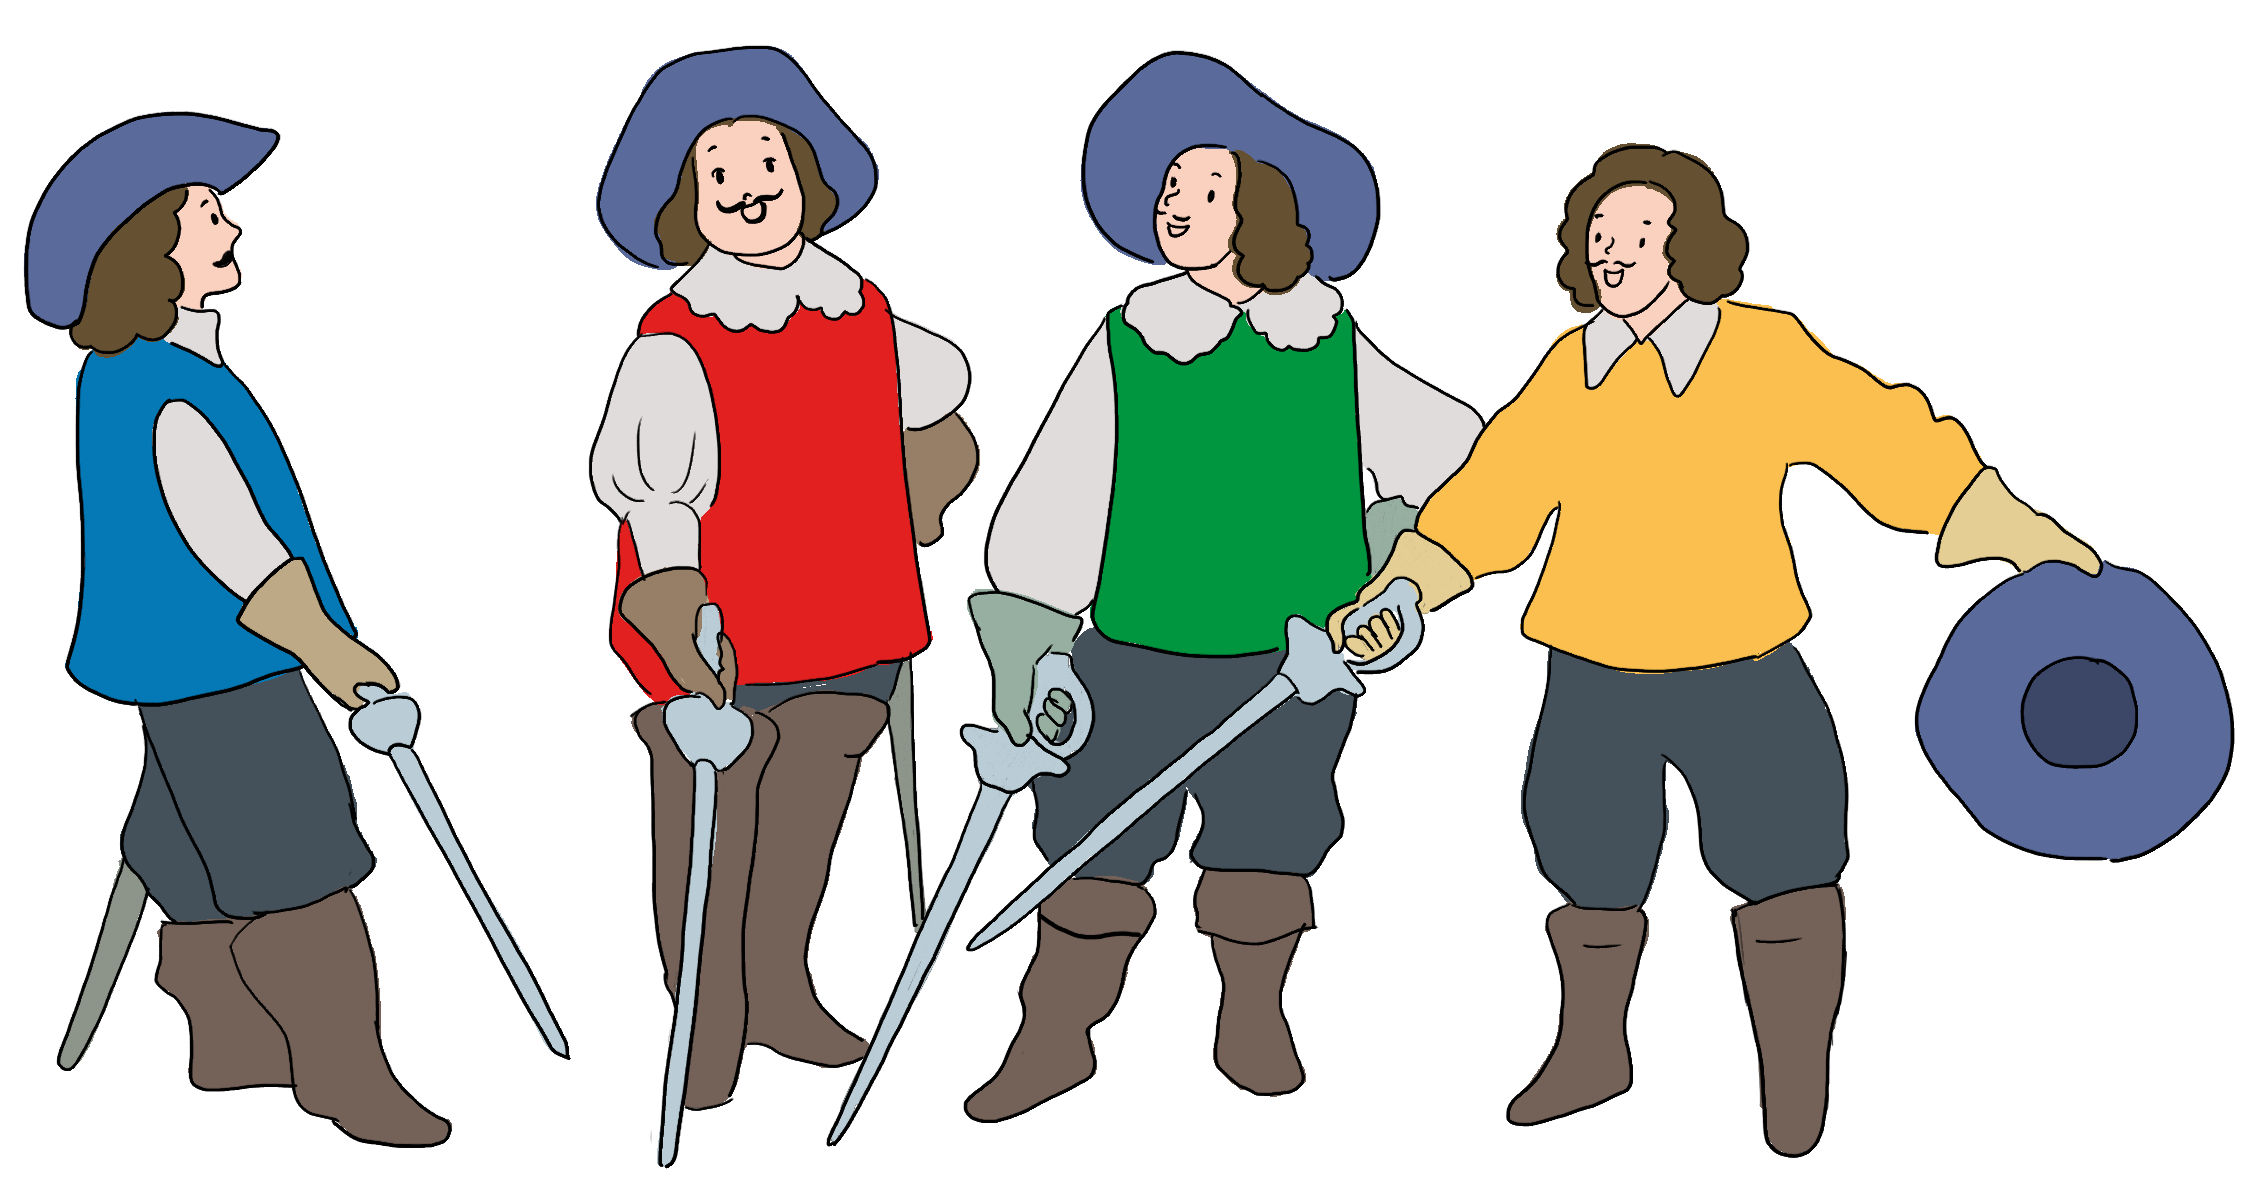
\includegraphics[width=1\linewidth]{Pi3_bai5}
		\vspace*{-15pt}
	\end{figure}
	\textit{Lời giải.} 	Tổng số vị trí của $4$ chàng ngự lâm là 
	\begin{align*}
		1+2+3+4 =10.
	\end{align*} 
	Từ điều kiện đầu tiên suy ra Aramis giữ vị trí thứ 
	\begin{align*}
		10-6 = 4.
	\end{align*}
	Từ điều kiện thứ hai suy ra Porthos giữ vị trí số $2$. Từ điều kiện cuối cùng suy ra Arthos giữ vị thứ thứ $3$, còn D'Artagnan giữ vị trí số~$1$.
	\vskip 0.1cm
	$\pmb{6.}$ Tại một khách sạn nọ, nhân viên trực quản lý điều hành phải làm việc từ $8$h sáng tới $8$h tối (phương án $A$), hoặc từ $8$h tối tới $8$h sáng (phương án $B$), hoặc làm trọn cả ngày $24$h bắt đầu từ $8$h (sáng hoặc tối) (phương án $C$). Nếu làm theo phương án $A$, nhân viên trực quản lý sẽ được nghỉ không ít hơn $1$ ngày ($24$h). Nếu làm theo phương án $B$, nhân viên trực quản lý sẽ được nghỉ không ít hơn $1$ ngày rưỡi ($36$h). Còn nếu làm theo phương án $C$, nhân viên trực quản lý sẽ được nghỉ không ít hơn hai ngày rưỡi ($60$h).
	\vskip 0.1cm
	Hỏi khách sạn phải cần có ít nhất bao nhiêu nhân viên trực quản lý để đảm bảo lịch làm việc, nghỉ ngơi ở trên được tuân thủ?
	\vskip 0.1cm
	\textit{Lời giải.} Rõ ràng thấy rằng khách sạn có thể chỉ cần $4$ nhân viên quản lý để điều hành theo sơ đồ làm việc ``một ngày làm, $3$ ngày nghỉ" theo phương án C--C--C--C.
	\vskip 0.1cm
	Ta sẽ chỉ ra rằng không thể bố trí với số nhân viên ít hơn $4$ người. Thật vậy, nếu có ai đó phải làm cả ngày ($24$h) thì trong thời gian anh ta nghỉ, vì không ai làm việc được quá $1$ ngày liền ($24$h), nên suốt thời gian nghỉ của anh ta là $2{.}5$ ngày, phải có ít nhất $3$ người khác thay phiên nhau làm việc.
	\vskip 0.1cm
	Nếu không có ai làm quá nửa ngày, thì do phải có ai đó làm việc vào ca đêm, nên khi anh ta nghỉ (ít nhất là $1{.}5$ ngày) phải có thêm ít nhất $3$ nhân viên quản lý khác phải làm thay thế.
	\vskip 0.1cm
	Vậy khách sạn cần có ít nhất $4$ nhân viên quản lý trực.
\end{multicols}
%\newpage
%\begingroup
%\thispagestyle{toancuabinone}
%\blfootnote{$^1$\color{toancuabi}Ottawa, Canada.}
%\AddToShipoutPicture*{\put(60,733){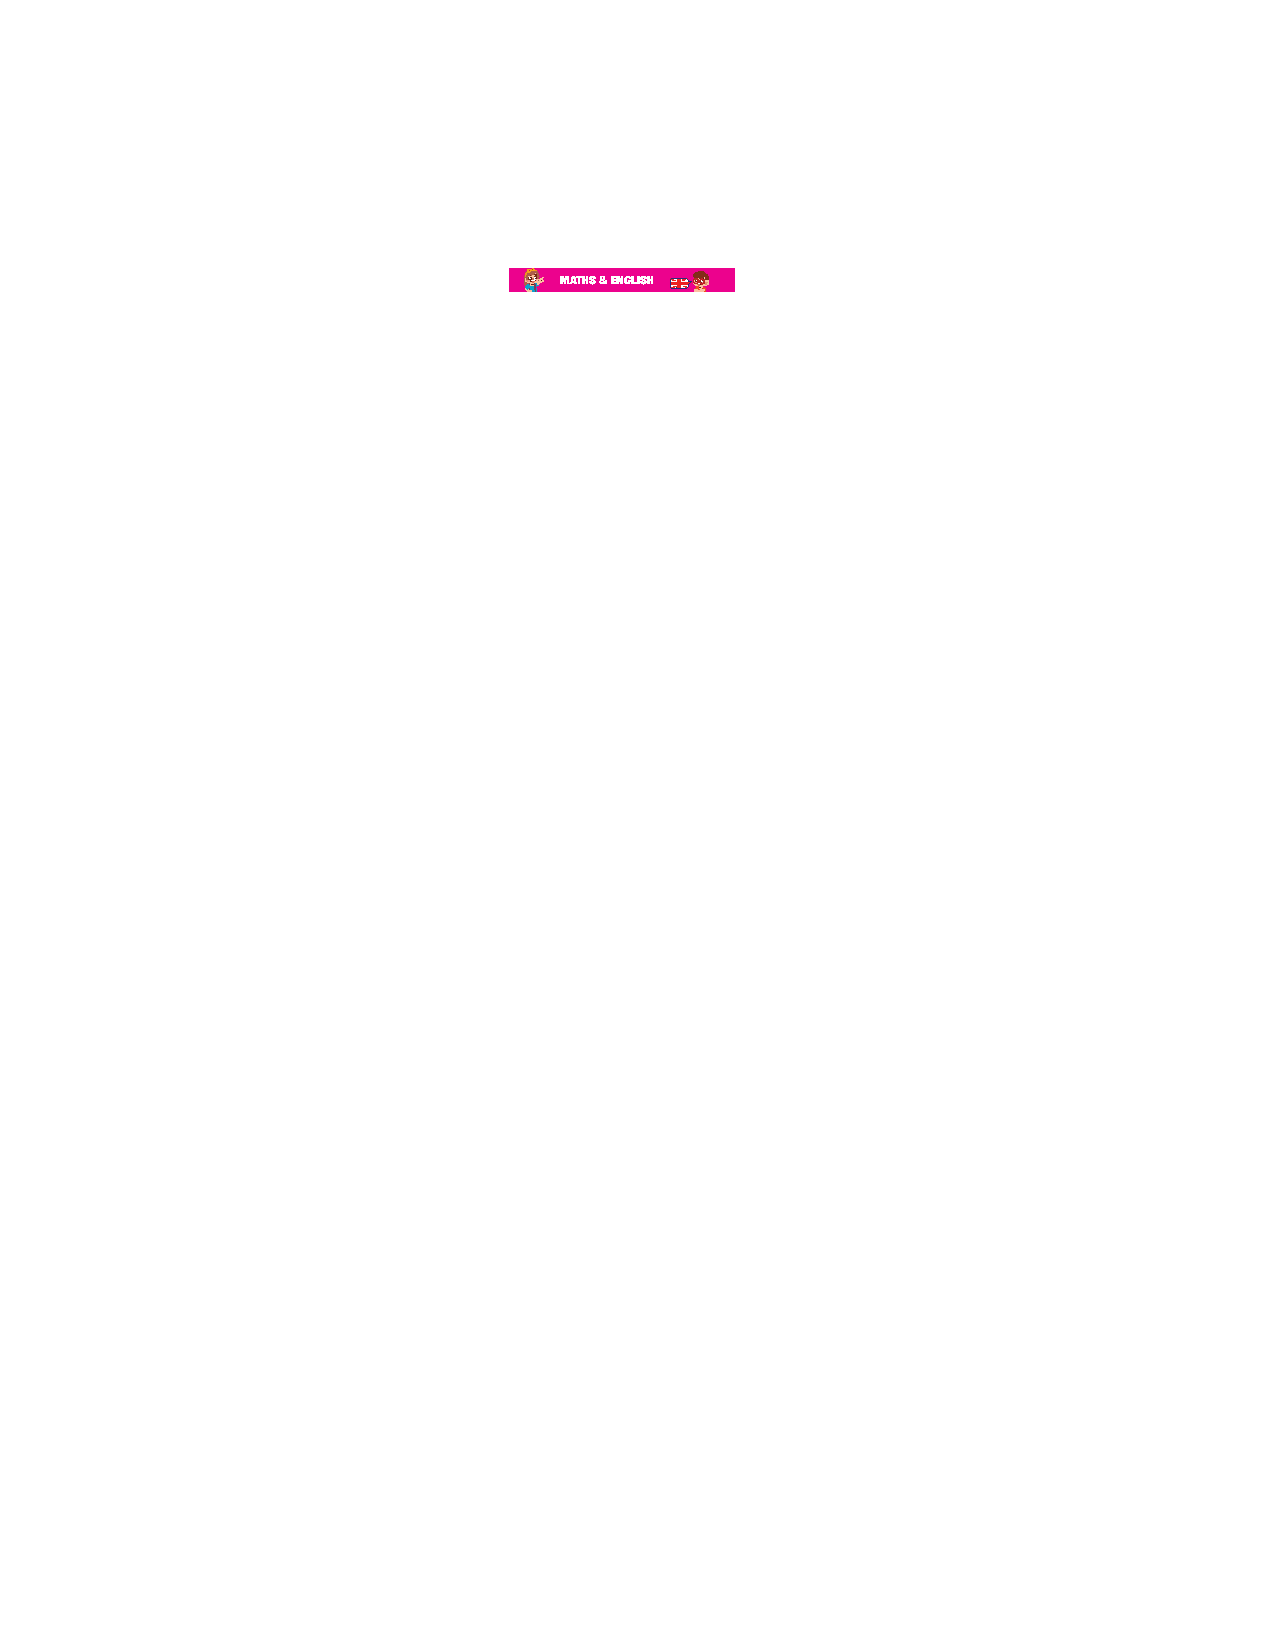
\includegraphics[width=17.2cm]{../mathc.pdf}}}
%%\AddToShipoutPicture*{\put(-2,733){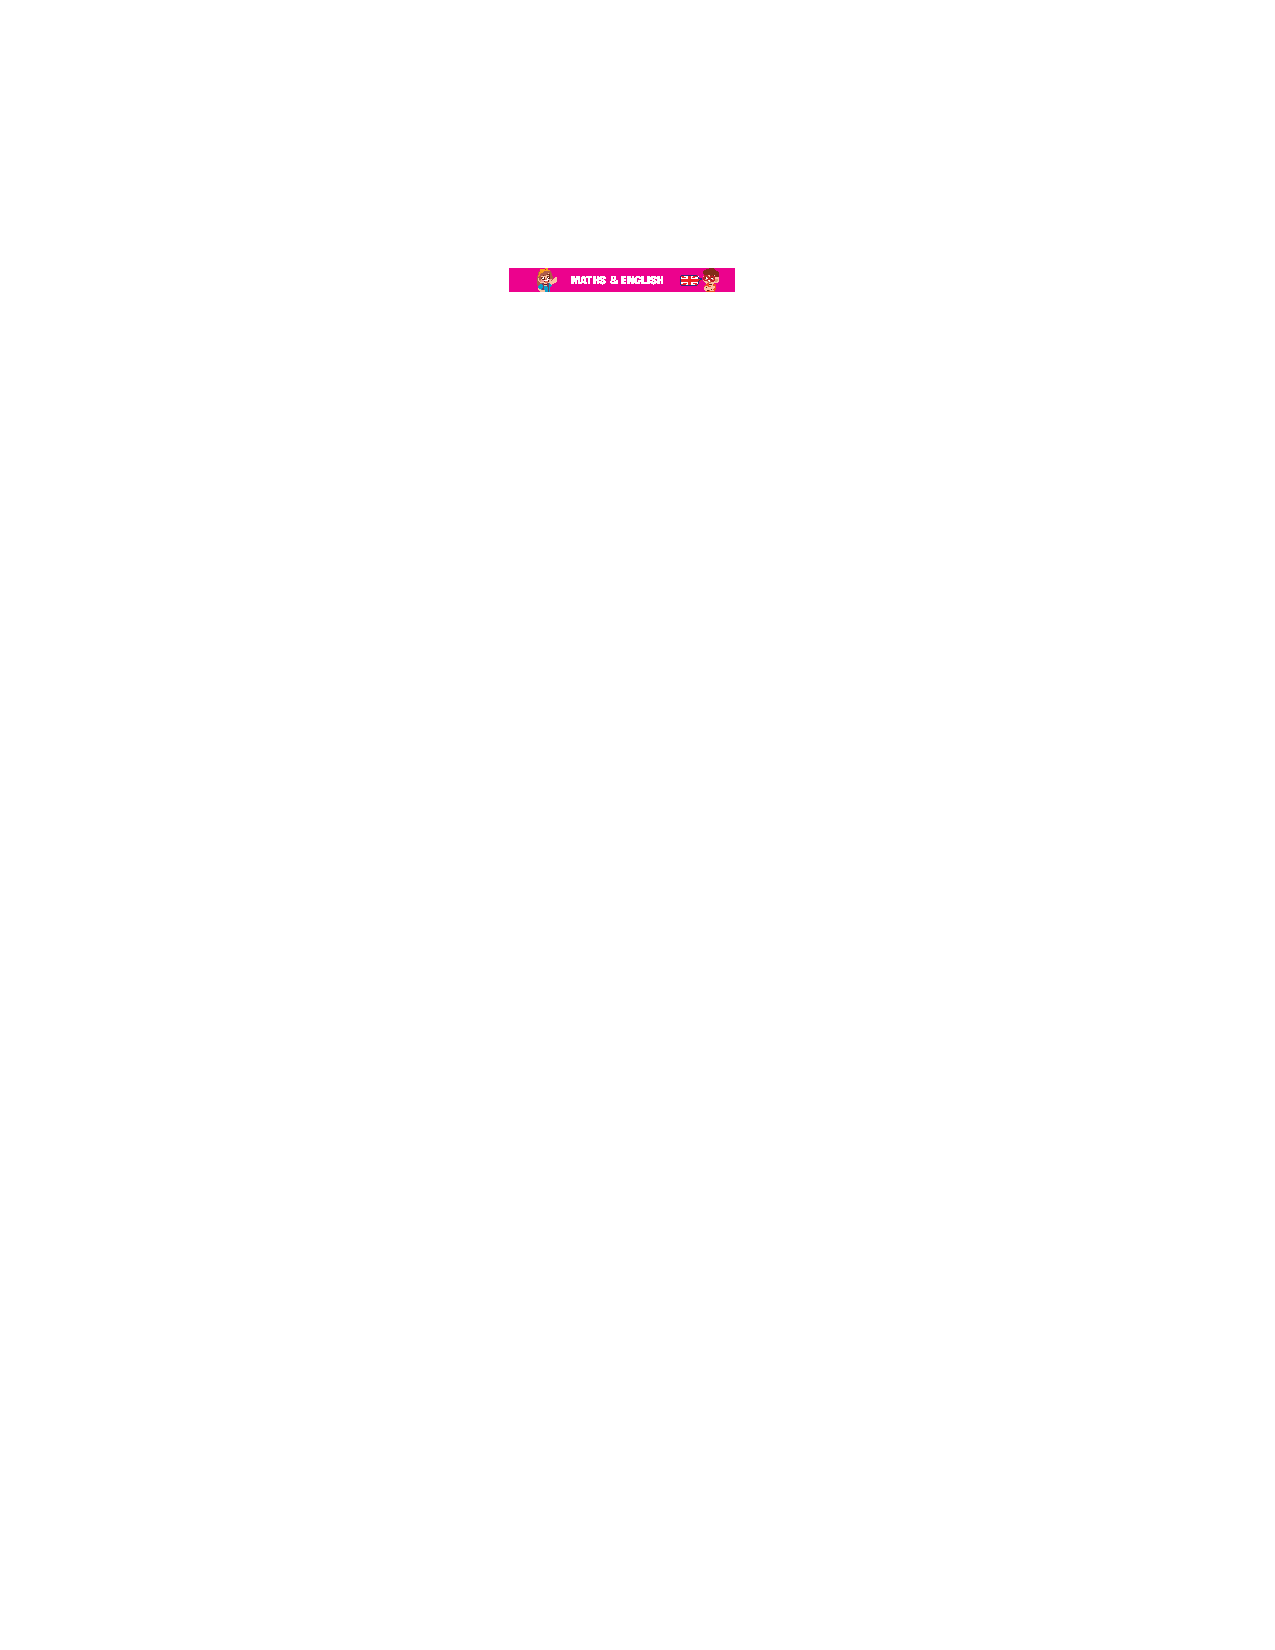
\includegraphics[width=17.2cm]{../mathl.pdf}}} 
%\AddToShipoutPicture*{\put(66,645){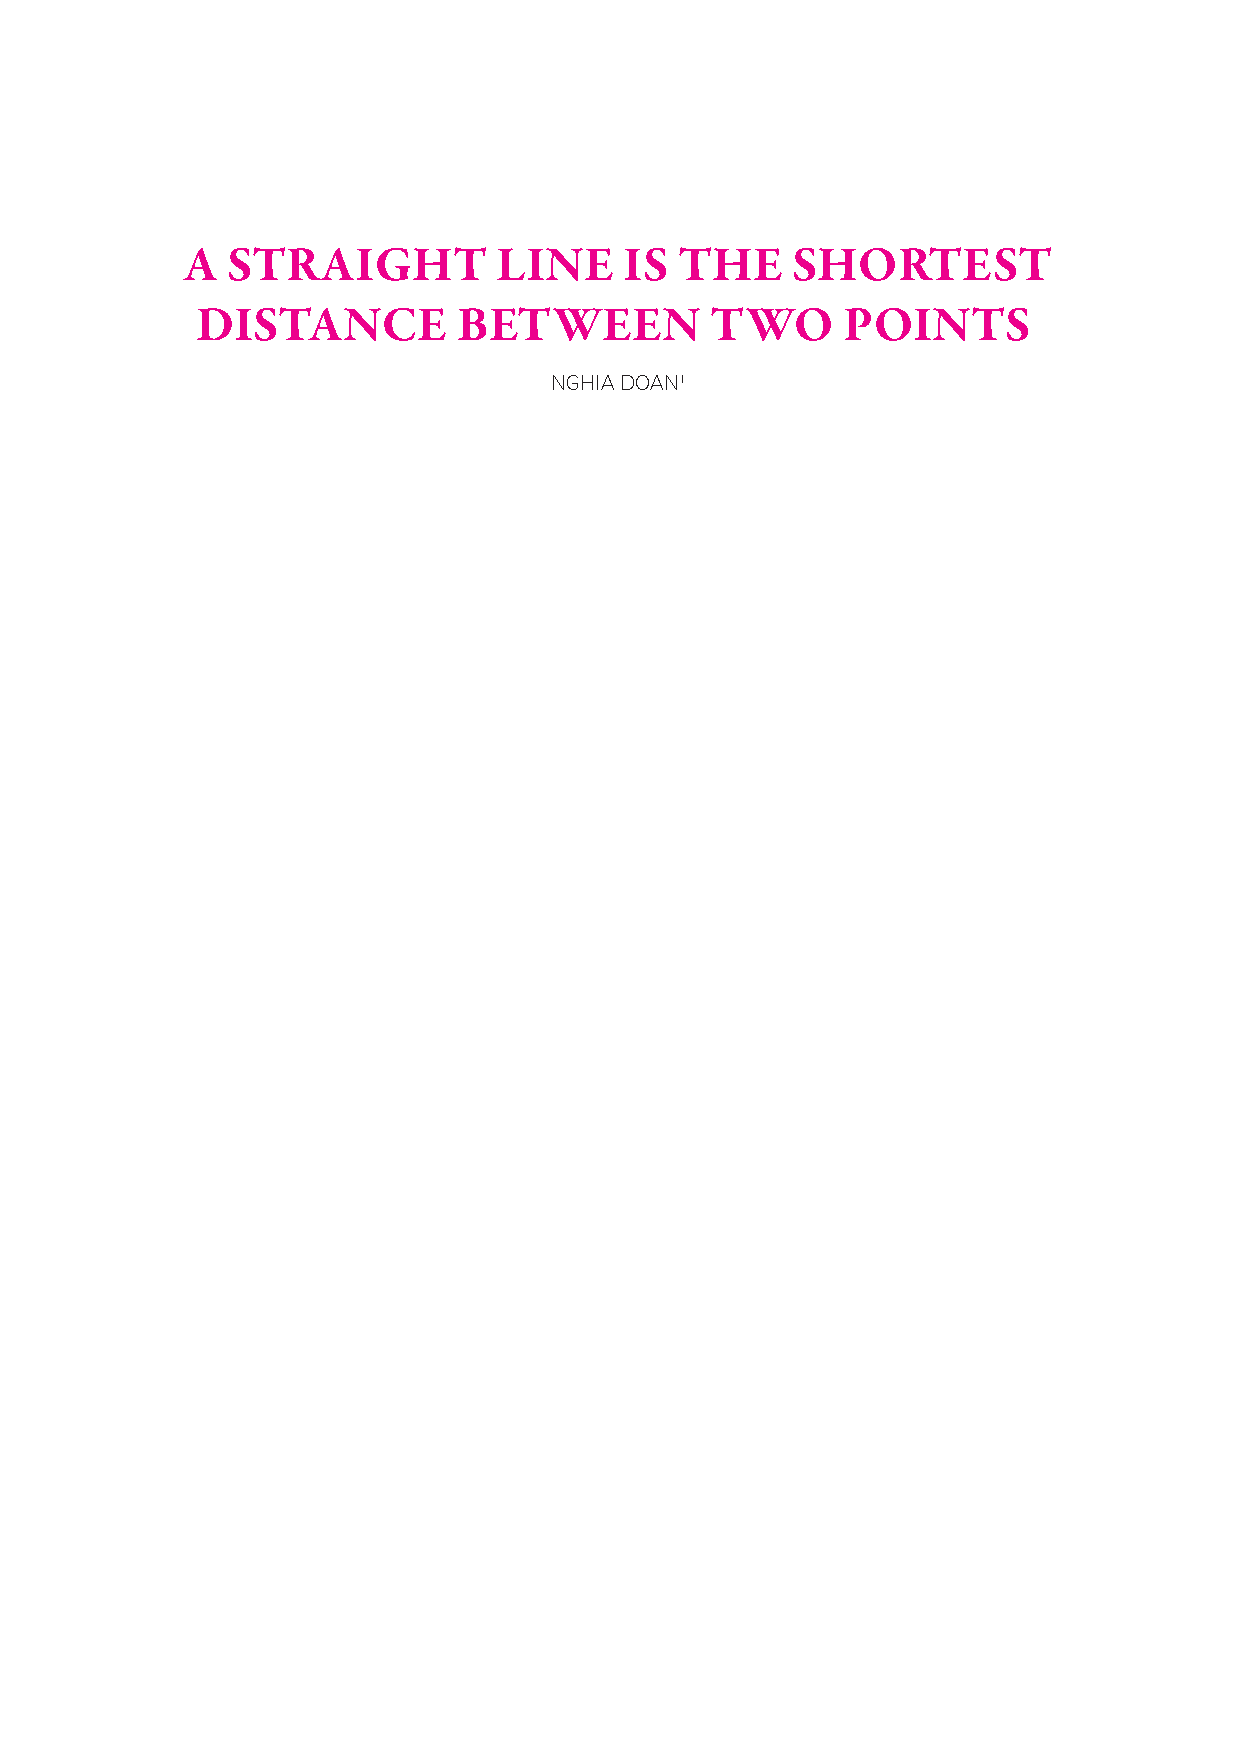
\includegraphics[scale=1]{../tieude5.pdf}}} 
%\centering
%\endgroup
%\graphicspath{{../toancuabi/pic/}}
%\vspace*{60pt}
%
%\begin{multicols}{2}
%	In this article, we explore some basic properties of broken lines.
%	\vskip 0.2cm
%	{\color{toancuabi}\textbf{Fact} (Triangle Inequality)\textbf{.}}
%	For any three points $A,B,C$, 
%	\begin{align*}
%		AB + BC \ge AC,
%	\end{align*}
%	The equality holds if and only if $A, B,$ and $C$ are collinear.
%	\vskip 0.1cm
%	{\color{toancuabi}\textbf{Fact} (Broken Line Inequality)\textbf{.}}
%	For any points $A_1,A_2,\ldots,A_n$, $A_1A_2 + A_2A_3 + \ldots + A_{n-1} A_{n} \ge A_1 A_n.$
%	The equality holds if and only if $A_1,A_2,\ldots,A_{n-1},$ and $A_n$ are collinear.
%	\vskip 0.2cm
%	\PIbox{ {\color{toancuabi}\textbf{Lemma} (Heron's Problem)\textbf{.}}
%		Two points $A$ and $B$ lie on one side of a straight line $l$.
%		$C$ is a point on on $l$.
%		The sum $CA+CB$ is minimal if and only if $C = BC' \cap \ell$, where $B'$ is the reflection of $B$ over $l$.}
%	\vskip 0.2cm
%	\begin{figure}[H]
%		\vspace*{-5pt}
%		\centering
%		\captionsetup{labelformat= empty, justification=centering}
%		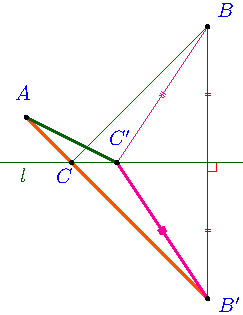
\includegraphics[width= 0.85\linewidth]{heron-problem-1.pdf}
%		\vspace*{-5pt}
%	\end{figure}
%	\vskip 0.1cm
%	\PIbox{ {\color{toancuabi}\textbf{Example} (Cross--section of a cube)\textbf{.}}
%		Lilian cuts a cube with side length $1.$ She got a with a  hexagon cross--section as shown below.
%		What is the minimal value of the hexagon perimeter $AB+BC+CD+DE+EF+FA$?}
%	\begin{figure}[H]
%		\vspace*{-5pt}
%		\centering
%		\captionsetup{labelformat= empty, justification=centering}
%		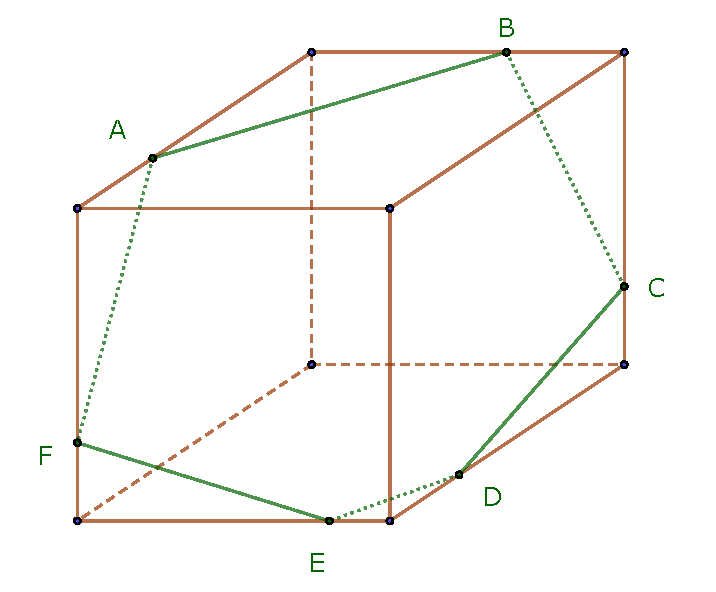
\includegraphics[width= 1\linewidth]{pi-2023-02-01.pdf}
%		\vspace*{-20pt}
%	\end{figure}
%	\textit{Solution.}
%	The diagram below is obtained by unfolding the cube into a net. The hexagon perimeter forms a broken line $ABCDEFA'.$
%	\begin{figure}[H]
%		\vspace*{-5pt}
%		\centering
%		\captionsetup{labelformat= empty, justification=centering}
%		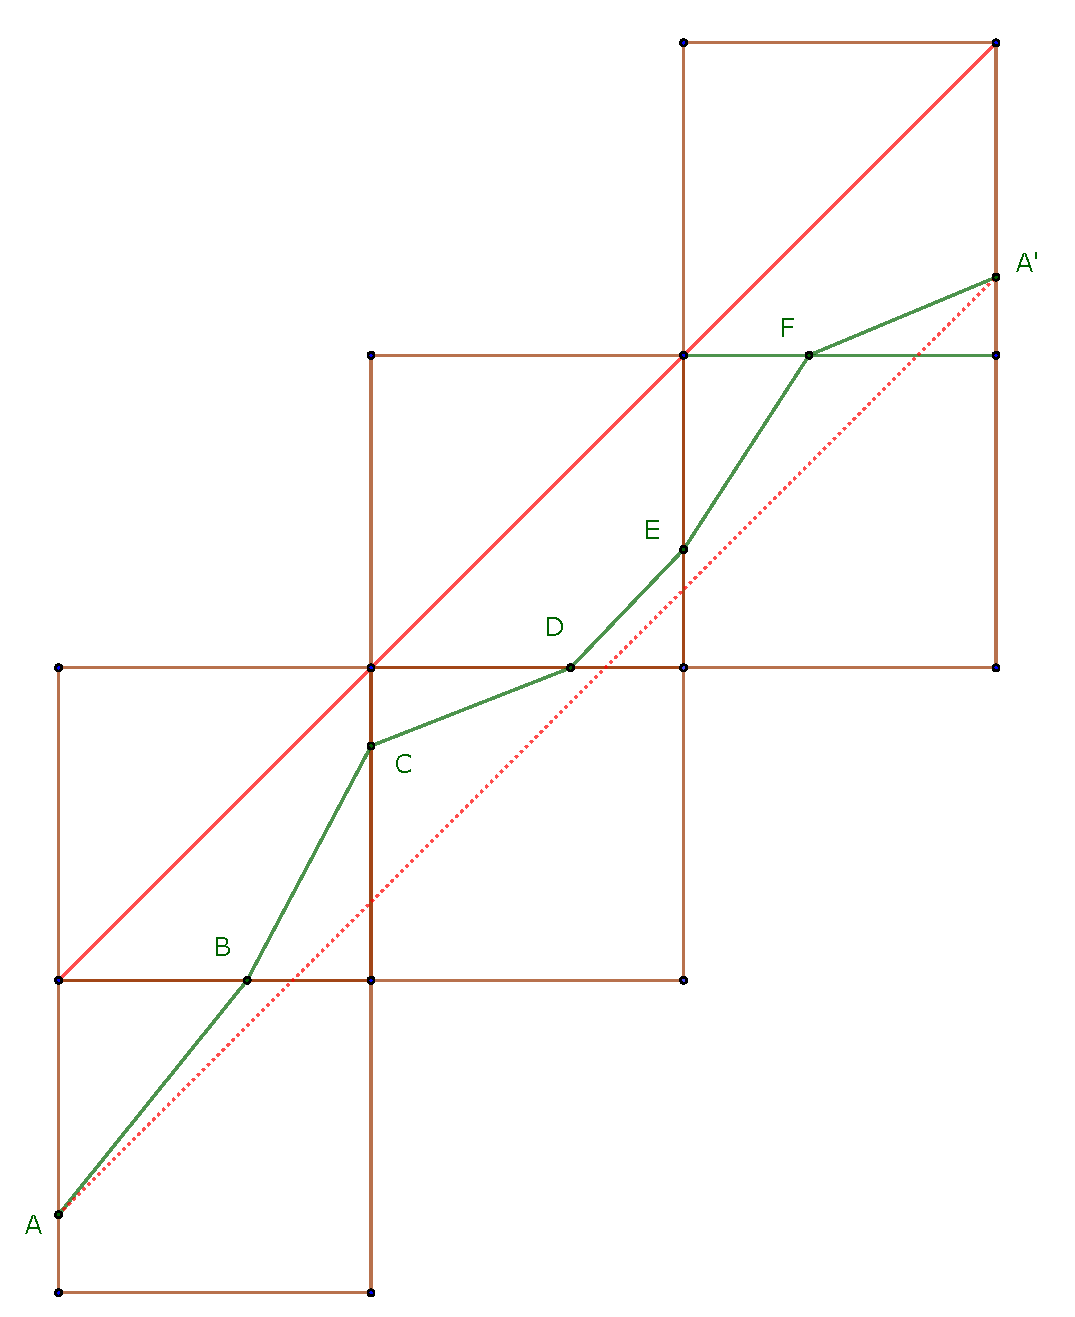
\includegraphics[width= 0.9\linewidth]{pi-2023-02-02.pdf}
%		\vspace*{-5pt}
%	\end{figure}
%	This is always larger or equal the distance $AA',$ which is same as three times the diagonal of the unit square.
%	Hence the perimeter is always at least ${3\sqrt{2}}.$
%	\vskip 0.2cm
%	\PIbox{{\color{toancuabi}\textbf{Example} (Diagonal of a hexagon)\textbf{.}}		
%		$ABCDEF$ is a convex hexagon, where $\angle A \ge 90\dg$ and $\angle D \ge 90\dg.$
%		Prove that $BC+CE+EF+FB\ge 2AD.$}
%	\vskip 0.2cm
%	\begin{figure}[H]
%		\vspace*{-5pt}
%		\centering
%		\captionsetup{labelformat= empty, justification=centering}
%		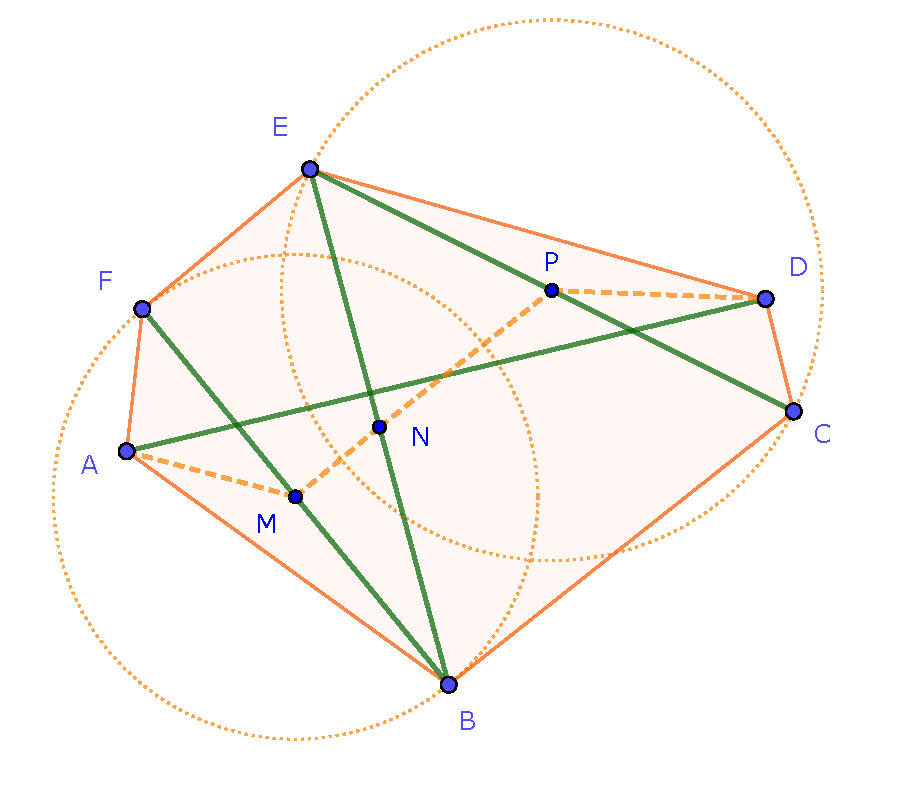
\includegraphics[width= 1\linewidth]{pi-2023-02-03.pdf}
%		\vspace*{-10pt}
%	\end{figure}
%	\textit{Proof}.
%	Let $M, N,$ and $P$ be the midpoints of $BF, BE,$ and $CE,$ respectively.
%	Since any broken line is longer or equal the distance between two endpoints, so $AD\le AM+MN+NP+PD.$
%	$MN$ is the median segment in $\triangle BEF,$ thus $FE = 2MN.$ Similarly $BC=2NP.$
%	In $\triangle ABF,$ $\angle A \ge 90\dg,$ thus $BF \ge 2AM.$ Similarly $CE \ge 2DP.$
%	Therefore $BC+CE+EF+FB \ge 2(AM+MN+NP+PD) = 2AD.$
%	\vskip 0.2cm
%	\PIbox{{\color{toancuabi}\textbf{Example} (Romanian Math Olympiad)\textbf{.}}
%		Let $ABCD$ be a convex quadrilateral. It is known that the circles with diameter $AB$ and $CD$ are externally tangent,
%		and so are the circles with diameters $AD$ and $BC.$
%		Prove that $ABCD$ is a rhombus.}
%	\begin{figure}[H]
%		\vspace*{-5pt}
%		\centering
%		\captionsetup{labelformat= empty, justification=centering}
%		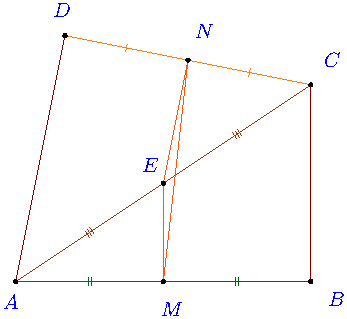
\includegraphics[width= 0.8\linewidth]{romanian-pb-gt-40.pdf}
%		\vspace*{-10pt}
%	\end{figure}
%	\textit{Proof}.
%	We first prove a claim.
%	\vskip 0.1cm
%	\textbf{\color{toancuabi}Claim.} Let $M$ and $N$ be the midpoint of $AB$ and $CD$, respectively, then $AD+ BC \ge 2MN.$
%	\vskip 0.1cm
%	\textit{Proof.}
%	Let $E$ be the midpoint of $AC.$ It is easy to see that 
%	\begin{align*}
%		MN \le ME+EN = \frac{BC}{2} + \frac{AD}{2} = \frac{AD+BC}{2}
%	\end{align*}
%	The equality can happen if and only if $MN$ intersect $AC$ at the midpoint of $AC$, so $MN \parallel AD \parallel BC.$
%	\vskip 0.1cm
%	By the claim $AD+BC \ge 2MN, \text{\ similarly\ } AB+CD \ge 2PQ,$ thus 
%	\begin{align*}
%		AB\!+\!BC\!+\!CD\!+\!DA \!\ge\! 2(MN+PQ). \tag{$*$}
%	\end{align*}
%	Now, let $P$ and $Q$ be the midpoints of $BC$ and $AD$, respectively.
%	Since the circles of diameters $AB$ and $CD$ are externally tangent so $AB+CD = 2MN,$ similarly $AD+BC = 2.$
%	Thus 
%	\begin{align*}
%		AB\!+\!BC\!+\!CD\!+\!DA \!=\! 2(MN+PQ). \tag{$**$} 
%	\end{align*}	
%	($**$) implies the existence of equality in ($*$), so $MN \parallel AD \parallel BC$ and $PQ \parallel AB \parallel CD$.
%	Thus $ABCD$ is a parallelogram, and $MN = AD = BC.$ Similarly $AB=CD.$ Since $AB +CD = 2MN$ (see above), therefore
%	\begin{align*}
%		AD = BC = MN = AB = CD.
%	\end{align*}
%	Hence, $ABCD$ is a rhombus.
%\end{multicols}
\newpage
\begingroup
\thispagestyle{toancuabinone}
\blfootnote{$^1$\color{toancuabi}Ottawa, Canada.}
\AddToShipoutPicture*{\put(60,733){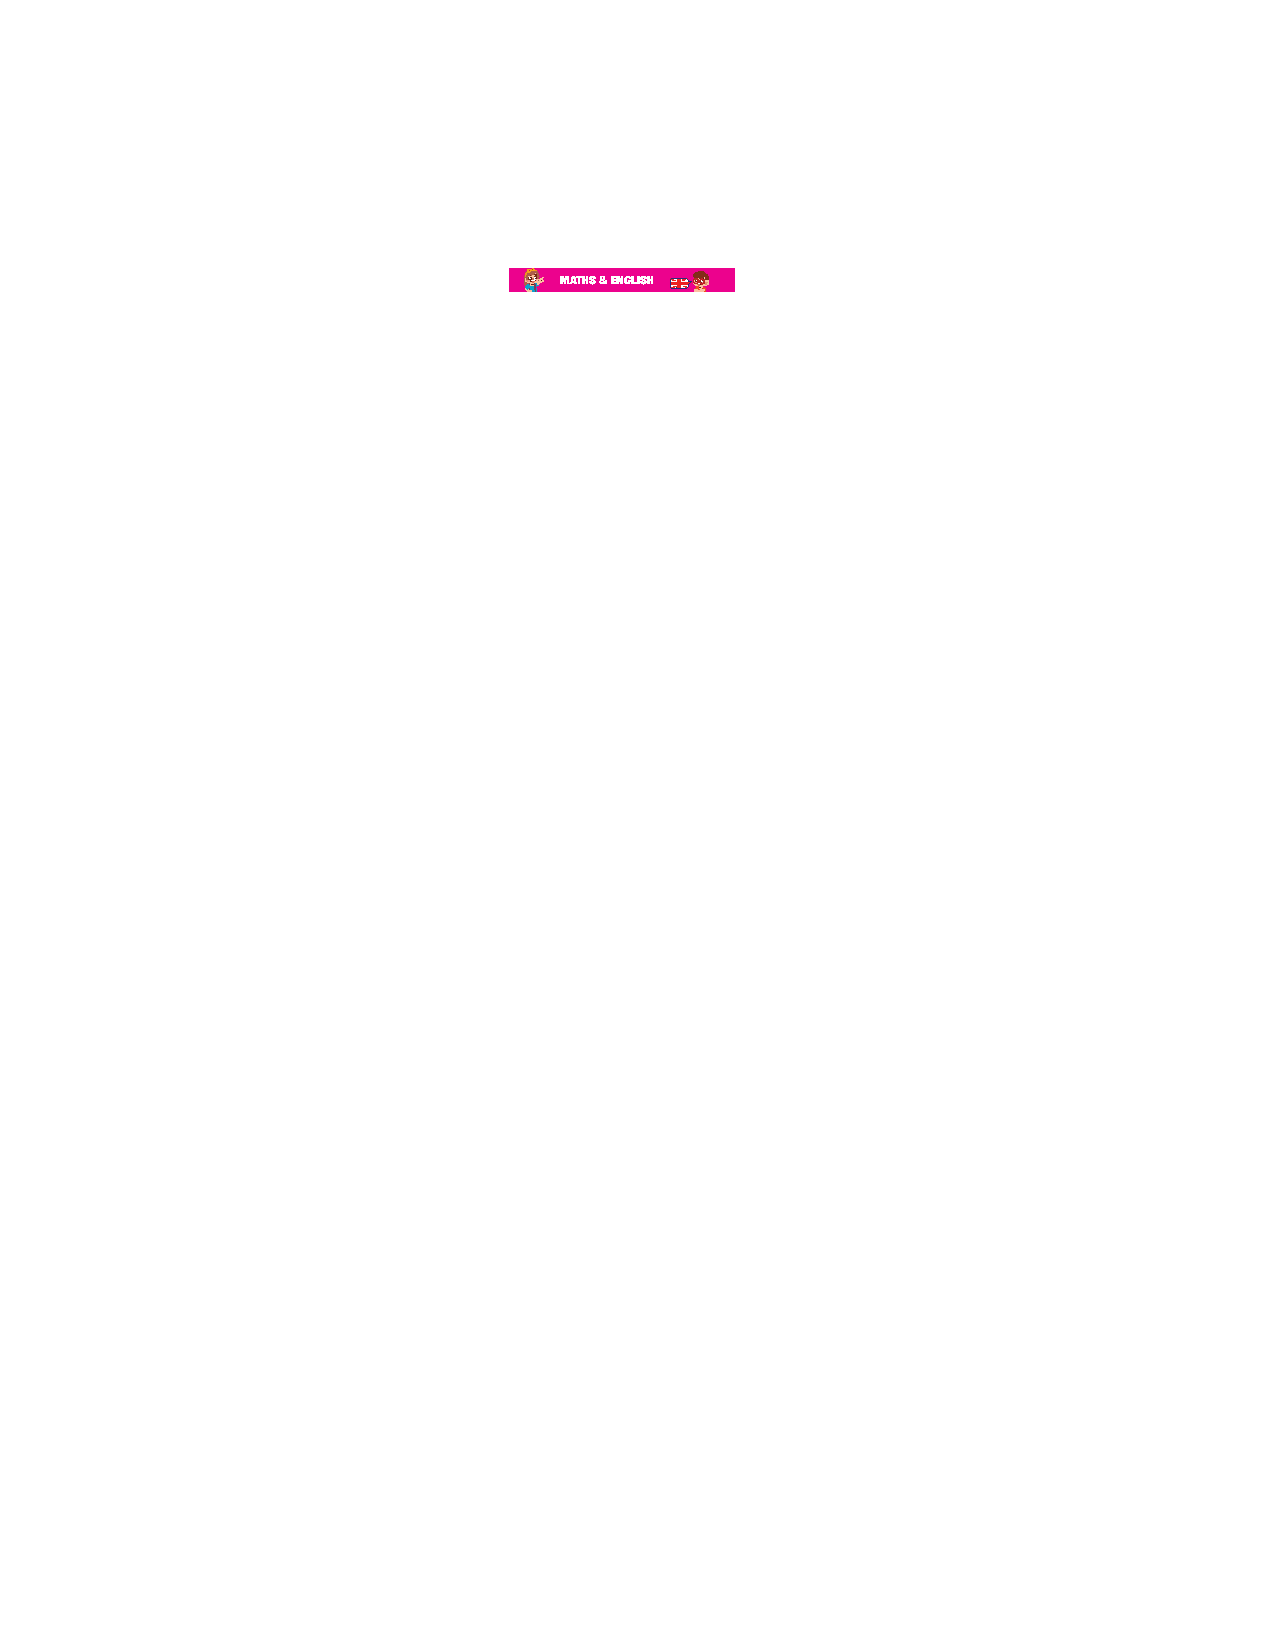
\includegraphics[width=17.2cm]{../mathc.pdf}}}
%\AddToShipoutPicture*{\put(-2,733){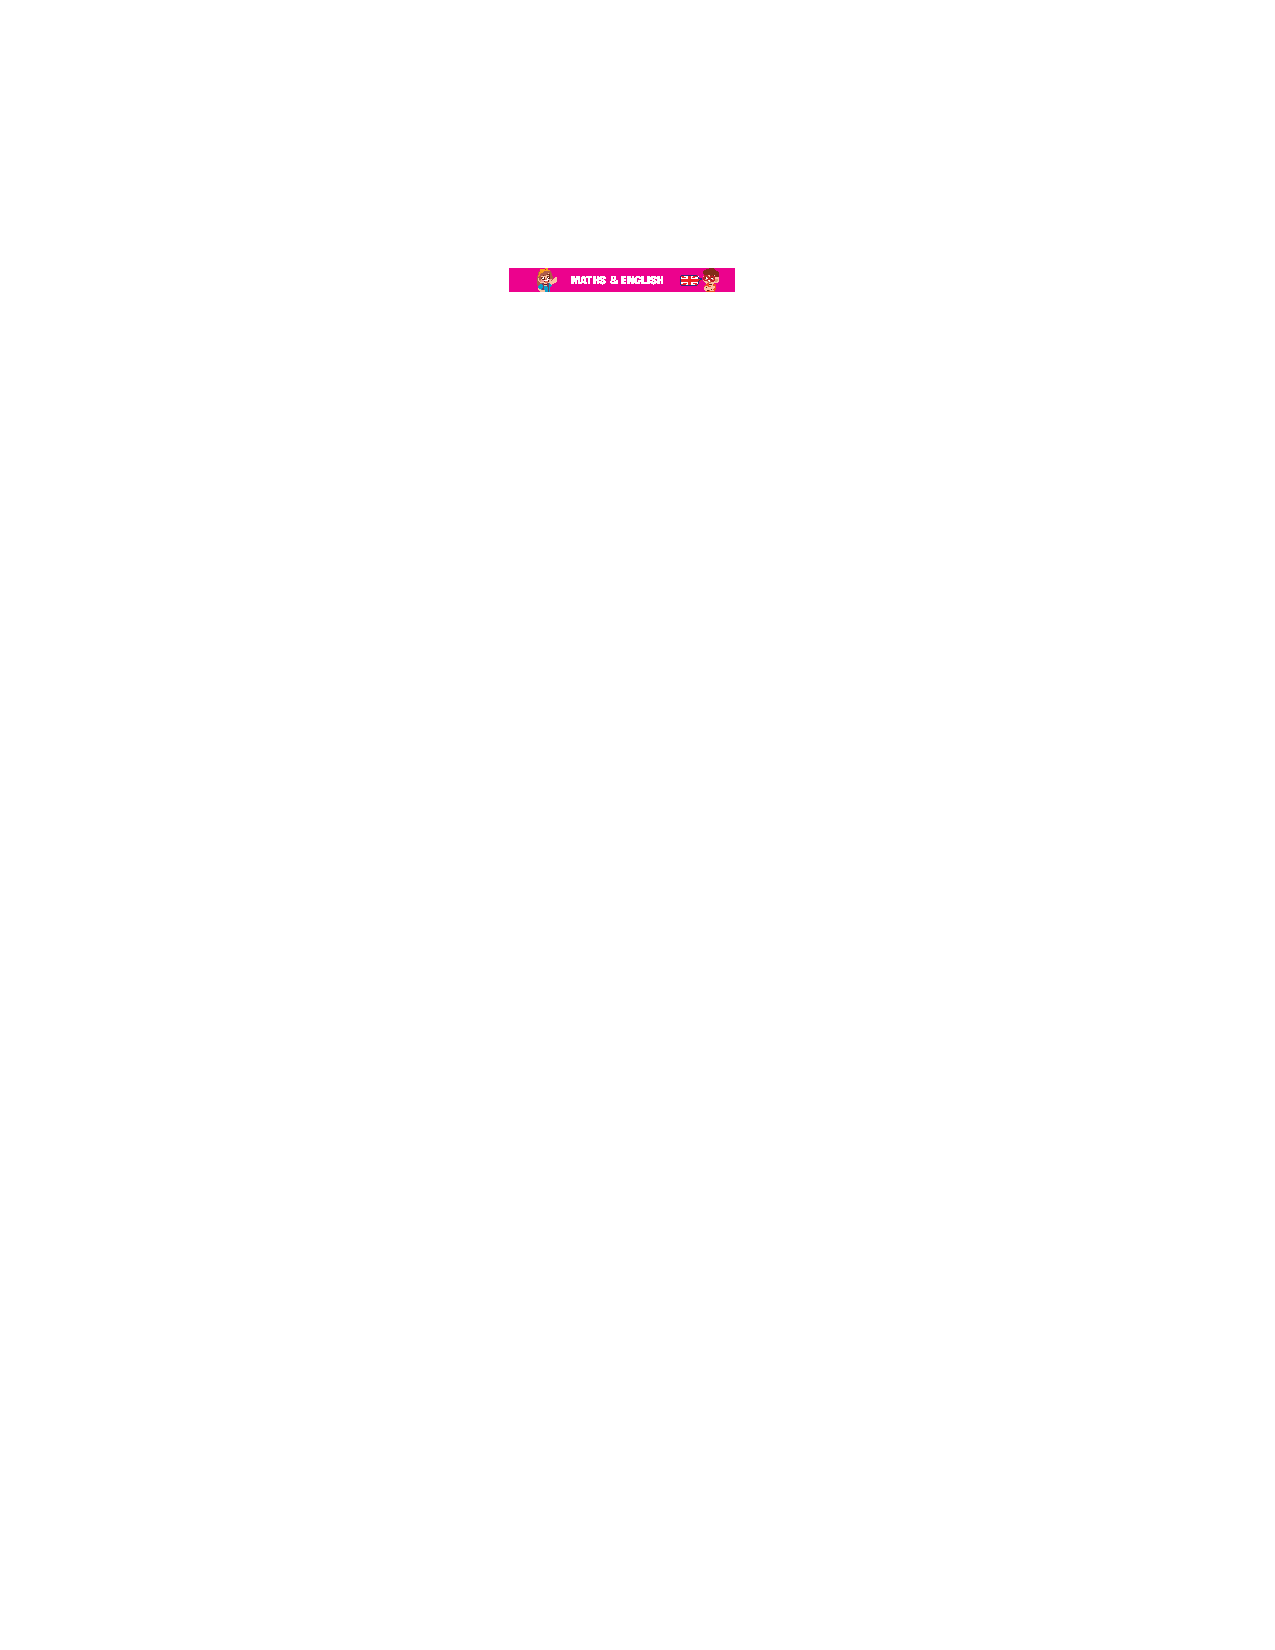
\includegraphics[width=17.2cm]{../mathl.pdf}}} 
\AddToShipoutPicture*{\put(170,675){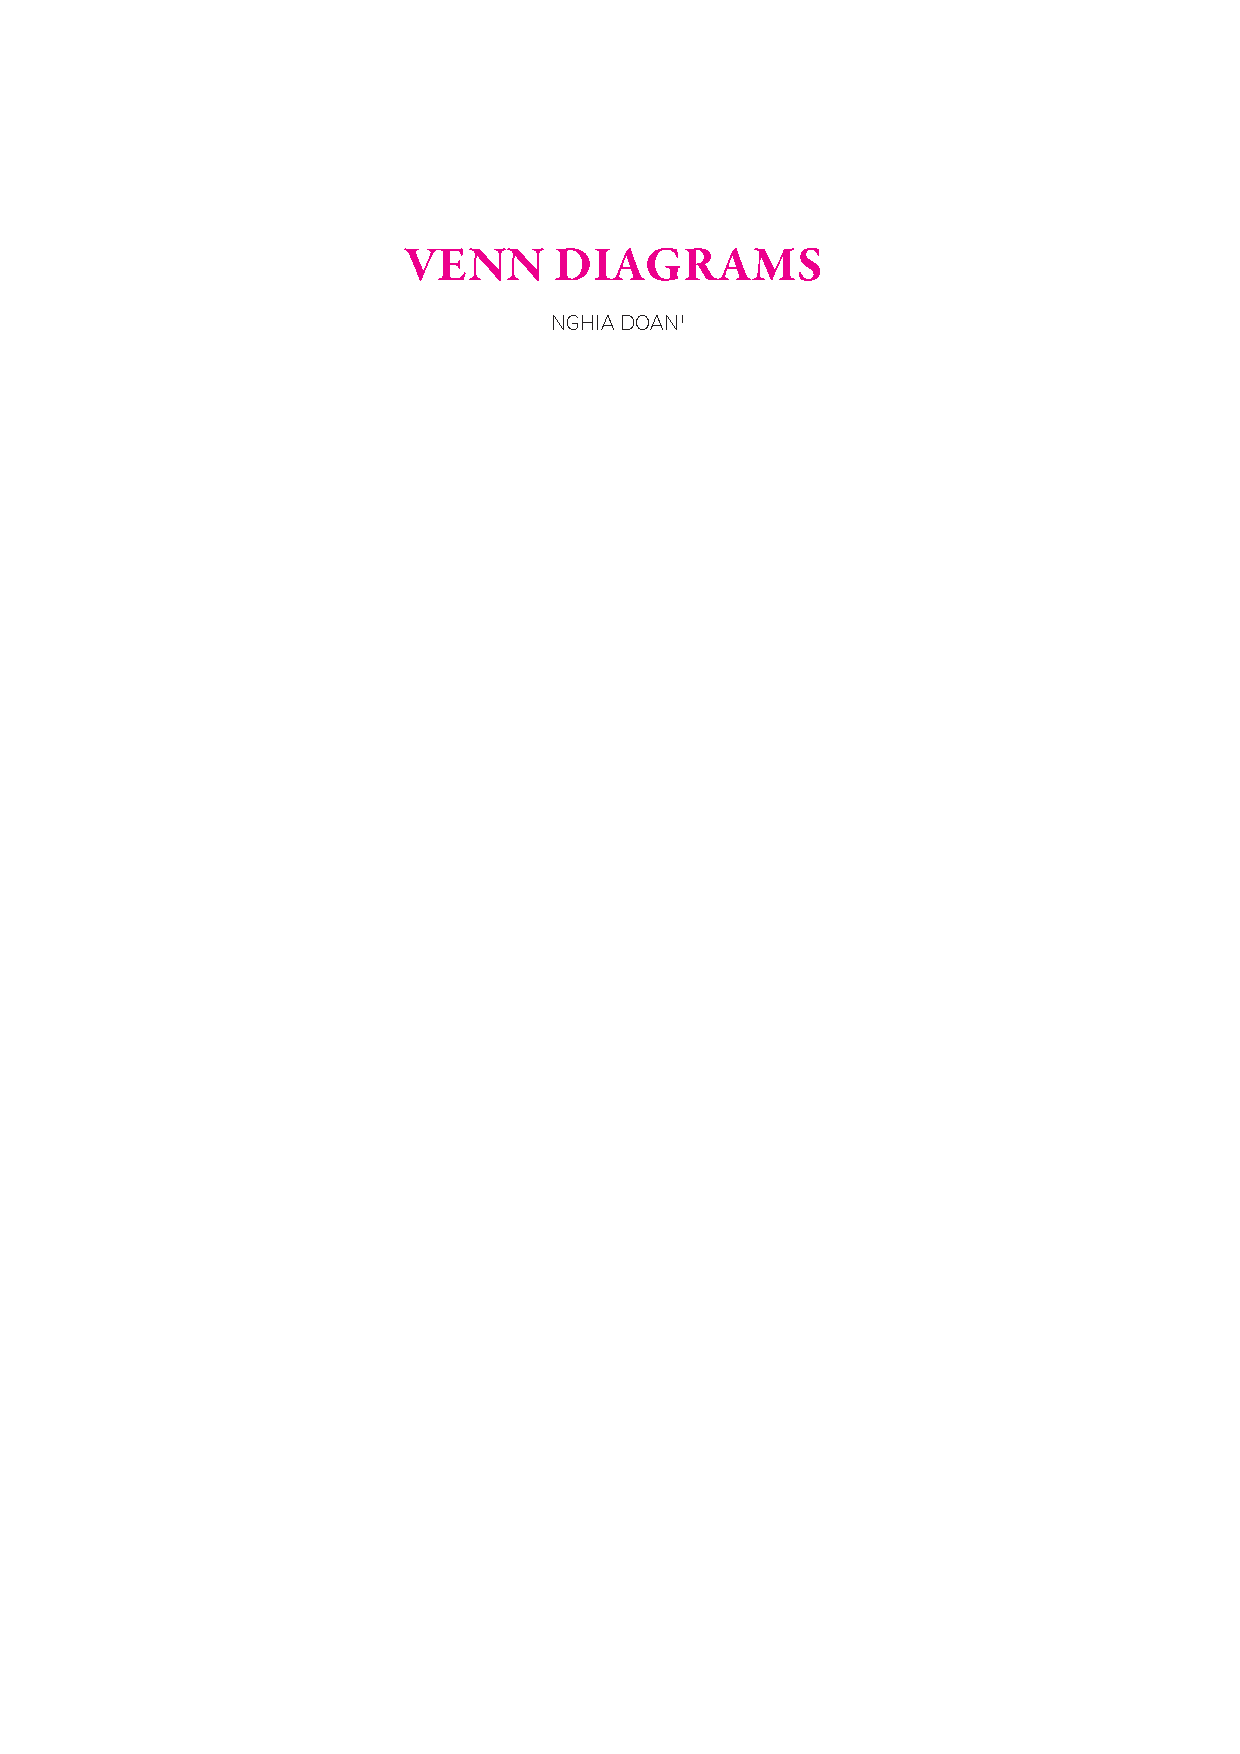
\includegraphics[scale=1]{../tieude4.pdf}}} 
\centering
\endgroup
\graphicspath{{../toancuabi/pic/}}
\vspace*{33pt}

\begin{multicols}{2}
	In this article, we explore the use of Venn diagrams through a few examples.
	\vskip 0.2cm
	\PIbox{{\color{toancuabi}\textbf{Example} (Overlapping rugs)\textbf{.}}
		Three rugs have a combined area of $200$ $m^2.$ The rugs are overlapped as shown in the diagram below.
		The overlapped rugs together cover a floor area of $140$ $m^2.$ Furthermore, the area covered by exactly any two rugs is $24$ $m^2$. 
		What is the total area covered by all the rugs?}
	\begin{figure}[H]
		\vspace*{-5pt}
		\centering
		\captionsetup{labelformat= empty, justification=centering}
		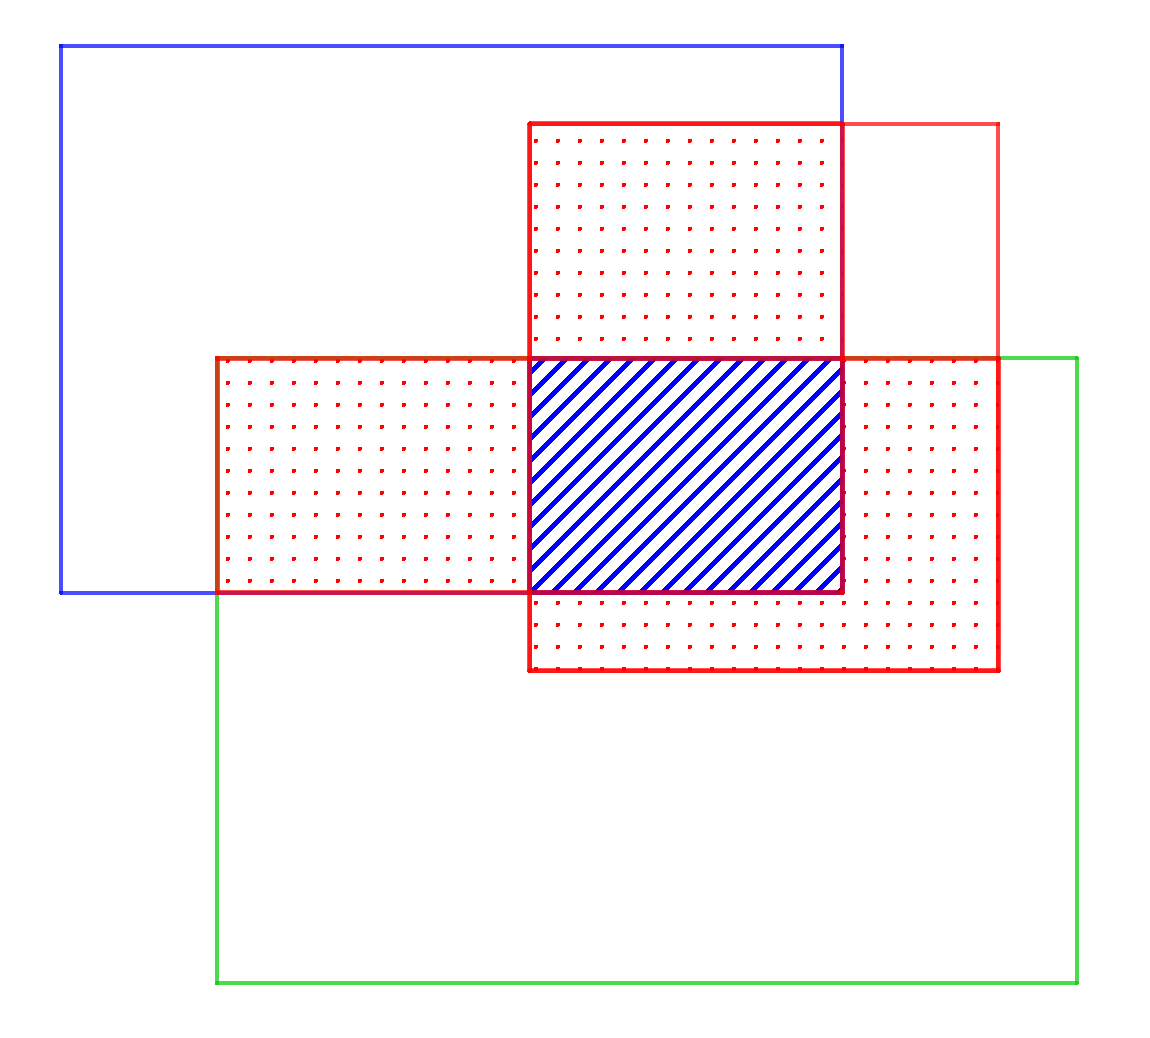
\includegraphics[width= 1\linewidth]{pi-2023-01-01.pdf}
		\vspace*{-15pt}
	\end{figure}
	\textit{Solution.}
	The total area of the three rugs, when not overlapping, is the sum of the areas of the three rectangles, which is $200$ $m^2.$
	The region shown in the above diagram is formed by the overlapping rugs and has a total area of $140$ $m^2.$
	This means that $200-140=60$ $m^2$ is the total area of the three \textcolor{red}{red dotted parts}
	(because they are where the rugs overlapped once) plus twice \textcolor{blue}{the blue hatch part}
	(because it is where the rugs overlapped twice).
	\vskip 0.1cm
	In other words, if $r$ and $b$ are the areas of a red dotted and the blue hatch, respectively, then $3r + 2b = 60.$
	Furthermore, since the area of a red dotted part plus the blue hatch part is $24$ $m^2,$ we have $r + b = 24.$
	Therefore $b = 3(r + b)- (3r+2b) = 3 \cdot 24 - 60 = 12.$
	\vskip 0.2cm
	\PIbox{
		{\color{toancuabi}\textbf{Exercise} (Overlapping circles)\textbf{.}}
		Three circles with radii $2$, $3$ and $4$ are overlapping each other.
		The largest circle is partitioned into the shaded region $A$ and two unshaded regions $B$ and $C$.
		If the total area of the shaded regions is $17 \pi$, what is the area of the region $A$?}
	\begin{figure}[H]
		\vspace*{-5pt}
		\centering
		\captionsetup{labelformat= empty, justification=centering}
		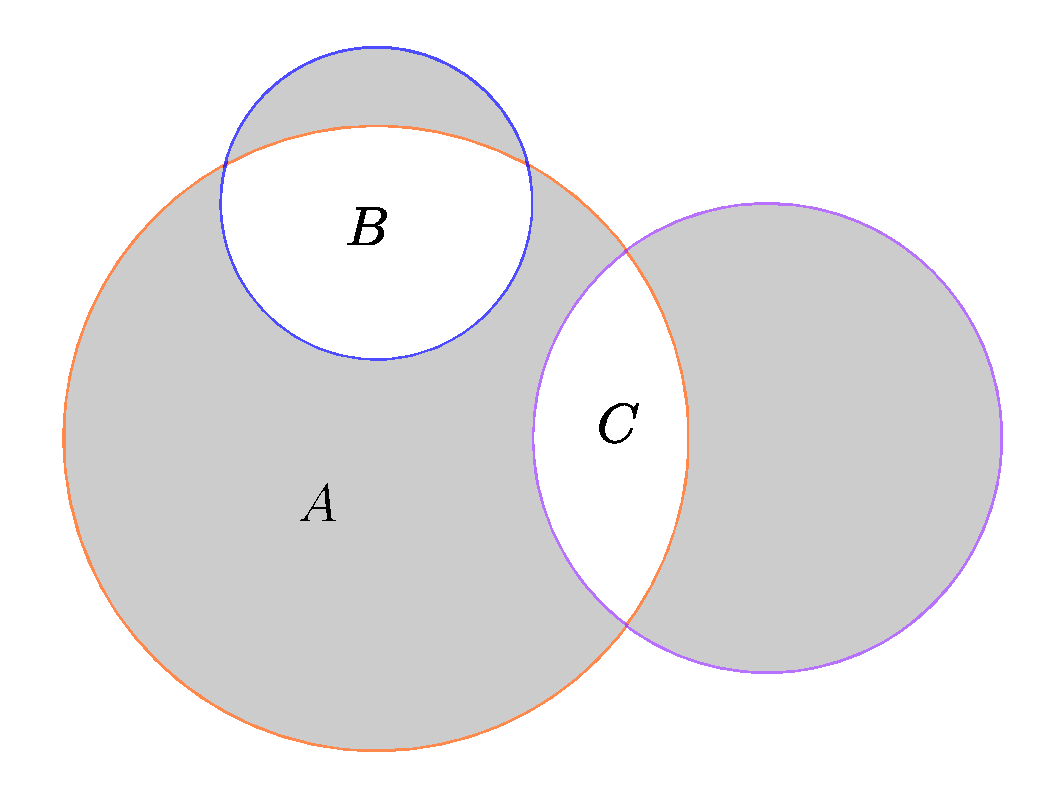
\includegraphics[width= 1\linewidth]{pi-2023-01-02.pdf}
		\vspace*{-15pt}
	\end{figure}
	\textit{Solution.}
	The total area of the three circles is the area of the shaded regions plus \textit{twice} the area of the unshaded regions:
	\begin{align*}
		&4\pi + 9\pi + 16\pi = 17\pi + 2(B+C) \\
		\Rightarrow \,&B+C = 6\pi \\
		\Rightarrow \,&A = 16\pi - (B+C) = 10\pi
	\end{align*}
	\vskip 0.2cm
	\PIbox{{\color{toancuabi}\textbf{Example} (Alligators are ferocious and creepy crawlers)\textbf{.}}
		If all alligators are ferocious creatures and some creepy crawlers are alligators. It is easy to verify that:
		(i) all alligators are creepy crawlers; (ii) some ferocious creatures are creepy crawlers;
		and (iii) some alligators are not creepy creatures.}
	
	\PIbox{
		Now, which statements below are true, false, or undecidable (you can't say it is true or false)?
		\vskip 0.1cm
		$S1.$ Some of creepy creatures are ferocious.
		\vskip 0.1cm
		$S2.$ Some ferocious creatures are creepy crawlers.
		\vskip 0.1cm
		$S3.$ Some alligators are not creepy creatures.
		\vskip 0.1cm
		$S4.$ Some ferocious crawlers are not alligators.
		\vskip 0.1cm
		$S5.$ Alligators are ferocious and creepy crawlers.}
	\vskip 0.2cm
	\textit{Solution.}
	To help the reasoning with visual cues, you can use Venn diagrams.
	\vskip 0.1cm
	First, we draw a \textcolor{red}{red circle} depicting the set of alligators. In other words all alligators are in this circle.
	Since all alligators are ferocious creatures, thus the \textcolor{blue}{blue circle} containing all ferocious creatures must cover the circle of alligators .
	Now, some creepy crawlers are alligators, thus the \textcolor{green}{green circle} containing all creepy crawlers must intersect and not contain the circle of alligators.
	Logically the circle of creepy crawlers then should intersect the circle of ferocious creatures and should not cover it.
	We get the diagram shown below.
	\begin{figure}[H]
		\vspace*{-5pt}
		\centering
		\captionsetup{labelformat= empty, justification=centering}
		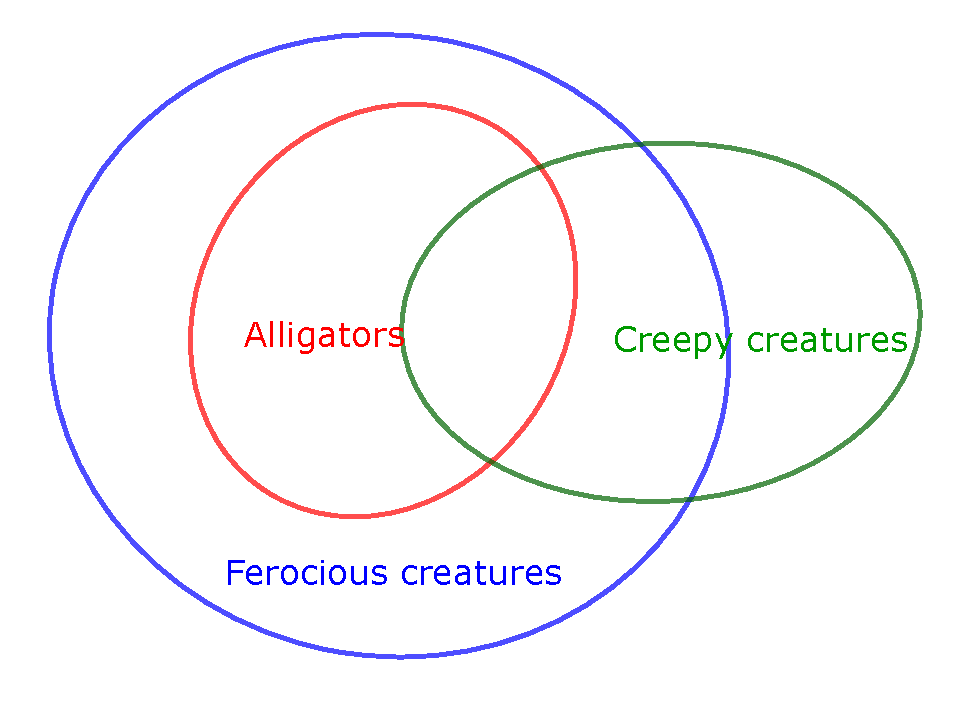
\includegraphics[width= 1\linewidth]{pi-2023-01-03.pdf}
		\vspace*{-10pt}
	\end{figure}
	For $S1,$ those creepy crawlers are alligators, they must be in the intersection of the \textcolor{red}{red circle} and \textcolor{green}{green circle}.
	Since the \textcolor{red}{red circle} resides within of the \textcolor{blue}{blue circle} the intersection must be part of the \textcolor{blue}{blue circle}.
	In other words, those creepy crawlers are ferocious creatures. Thus the statement $S1$ is true.
	\vskip 0.1cm
	It is also easy to verify that $S2$ is true.
	\vskip 0.1cm
	Since we know that \textit{some creepy crawlers are alligators}, thus the \textcolor{green}{green circle} intersect
	and may not contain the whole the \textcolor{red}{red circle}, thus $S2$ is \textit{undecidable.}
	We don't know if some alligators are not creepy.
	\vskip 0.1cm
	The remaining two statements $S4$ and $S5$ are both \textit{undecidable}. Try to prove it yourself.
	\vskip 0.1cm
	\PIbox{{\color{toancuabi}\textbf{Exercise} (Are boys good at math)\textbf{.}}
		Let us assume that \textit{all boys in the math club are good at math.} 
		Which of the following statements must be true?
		\vskip 0.1cm
		$S1.$ No boy whose math is not good is a member of the math club.
		\vskip 0.1cm
		$S2.$ All boys whose math is good are members of the math club.
		\vskip 0.1cm
		$S3.$ All boys who are not members of the math club are not good at math.
		\vskip 0.1cm
		$S4.$ Every member of the math club whose math is good is a boy.
		\vskip 0.1cm
		$S5.$ There is one boy in the math club whose math is not good.
		\vskip 0.1cm
		Now decide whether the following is true or false.
		\textit{A girl is good at math as a boy who is not member of the math club is not good as math as a boy who is member of the math club.}}
	\vskip 0.1cm
	\textit{Solution.}
	Draw three circles that are pairwise intersecting. One circle is labeled \textit{boys}; the girls are outside of this circle. One circle is labeled \textit{math} meaning whoever in this circle is good at math; the students outside of this circle are not good at math. One circle is labeled \textit{club} meaning whoever in this circle is a member of the math club; the students outside of this circle are not members of the math club.
	None of the circles can contain another one. The \textit{club} circle must contain the inversection of the \textit{boys} circle and the \textit{math} circle.
	A diagram is shown below.
	\begin{figure}[H]
		%			\vspace*{-5pt}
		\centering
		\captionsetup{labelformat= empty, justification=centering}
		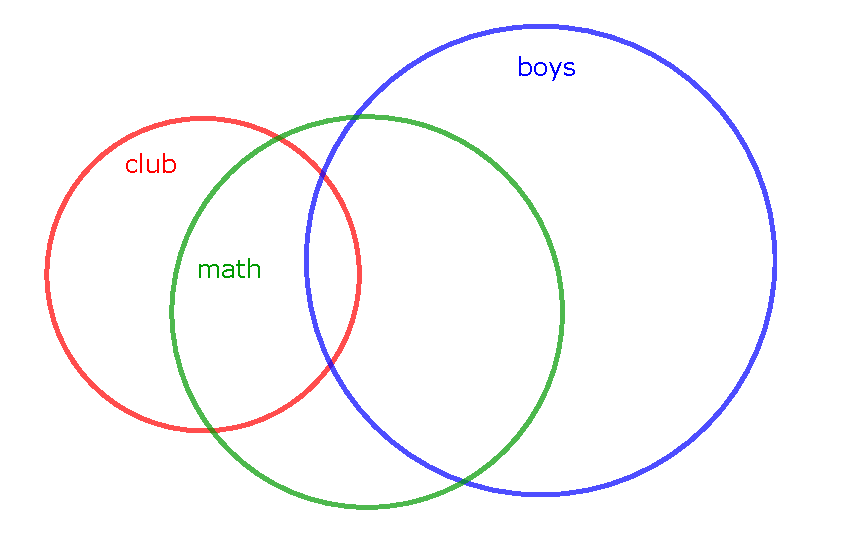
\includegraphics[width= 1\linewidth]{pi-2023-01-04.pdf}
		\vspace*{-10pt}
	\end{figure}
	For $S2,$ $S3,$ $S4,$ and $S5,$ it is easy to find a counterexample, thus none of them is true.
	The statement $S1$ means that if a boy is not good at math, then he is not a member of the math club. This is obviously true. We conclude that $S1$ is true.
	\vskip 0.1cm
	\columnbreak
	\PIbox{
	\centerline{\textbf{\color{toancuabi}Vocabulary}}
	\vskip 0.1cm
	{\color{toancuabi}Venn diagram (n):} sơ đồ Venn, biểu đồ Venn
	\vskip 0.1cm
	{\color{toancuabi}intersection (n):} phần giao nhau
	\vskip 0.1cm
	{\color{toancuabi}overlapping (adj):} chồng lên nhau
	\vskip 0.1cm
	{\color{toancuabi}furthermore (adv):} hơn nữa
	\vskip 0.1cm
	{\color{toancuabi}undecidable (adj):} không xác định được tính đúng/sai
	\vskip 0.1cm
	{\color{toancuabi}suppose (v):} giả sử 
	\vskip 0.1cm
	{\color{toancuabi}suppose by contradiction (v):} giả sử bằng phản chứng 
	\vskip 0.1cm
	{\color{toancuabi}rug (n):} tấm thảm
	\vskip 0.1cm
	{\color{toancuabi}alligator (n):} cá sấu
	\vskip 0.1cm
	{\color{toancuabi}ferocious (adj):} hung dữ
	\vskip 0.1cm
	{\color{toancuabi}creepy (adj):} rùng rợn
	\vskip 0.1cm
	{\color{toancuabi}crawler (n):} loài bò sát
	\vskip 0.1cm
	{\color{toancuabi}creature (n):} sinh vật}
\end{multicols}
\newpage
\begingroup
\blfootnote{$^1$\color{toancuabi}Trường Liên cấp Hội nhập Quốc tế iSchool Quảng Trị.}
\AddToShipoutPicture*{\put(48,680){
\includegraphics[scale=1]{../tieude10.pdf}}}   
\centering
\endgroup
\vspace*{30pt} 

\begin{multicols}{2}
	\textbf{\color{toancuabi}Ayatori} (hay trò chơi dây) là một trò chơi mà khi nhắc đến chắc chắn những người hâm mộ bộ truyện tranh Doraemon đều biết đến và nhớ ngay tới nhân vật Nobita. Trò chơi Ayatori là một trò chơi rất thú vị, người chơi sẽ sử dụng một sợi dây được buộc thành hình tròn, sau đó dùng những ngón tay của mình đan xen các sợi dây để tạo ra nhiều hình dạng khác nhau từ đơn giản đến phức tạp. Hôm nay, em hãy thử xếp hình ngôi sao thông qua trò chơi Ayatori nhé!
	\vskip 0.1cm
	\textit{Bước} $1$: Cách cầm dây khi mới bắt đầu chơi trò chơi Ayatori là giữ sợi dây trong ngón cái và ngón út bằng hai tay, rồi kéo ngang để chuẩn bị chơi.
	\begin{figure}[H]
		\vspace*{-10pt}
		\centering
		\captionsetup{labelformat= empty, justification=centering}
		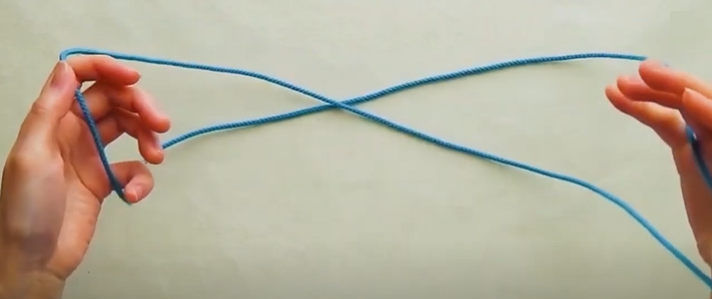
\includegraphics[width=0.81\linewidth]{1a}
		
		\vspace*{1pt}
		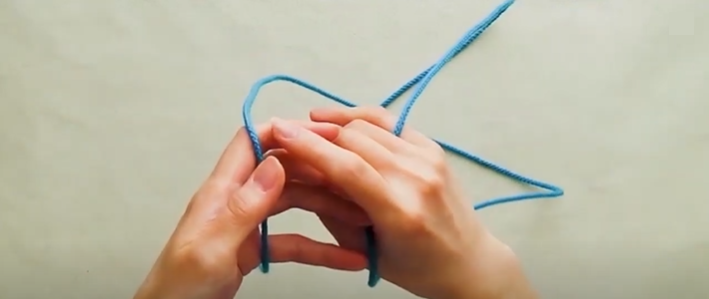
\includegraphics[width=0.81\linewidth]{1b}
		
		\vspace*{1pt}
		\hspace*{1pt}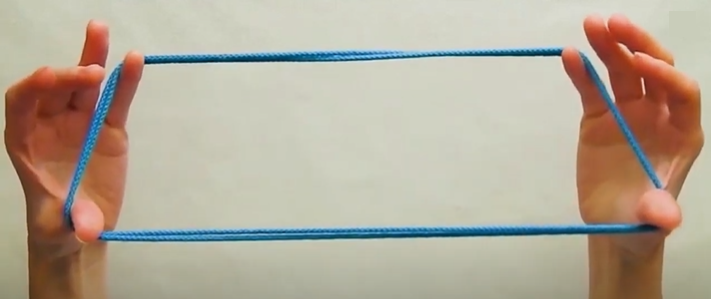
\includegraphics[width=0.81\linewidth]{1c}
		\vspace*{-10pt}
	\end{figure}
	\textit{Bước} $2$: Thả dây ở hai ngón tay út. Sau đó dùng hai ngón tay út luồn phía dưới sợi dây ở hai ngón cái để kéo sợi dây ra như hình vẽ.
	\begin{figure}[H]
		\vspace*{-5pt}
		\centering
		\captionsetup{labelformat= empty, justification=centering}
		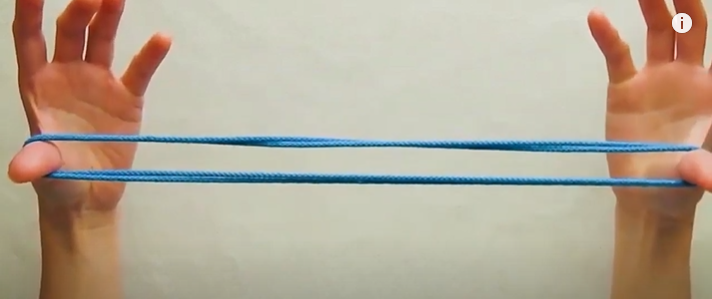
\includegraphics[width=0.81\linewidth]{2a}
%		\vspace*{-5pt}
	\end{figure}
	\begin{figure}[H]
		\vspace*{5pt}
		\centering
		\captionsetup{labelformat= empty, justification=centering}
		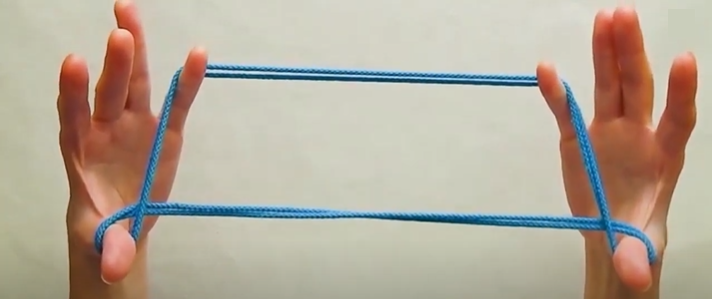
\includegraphics[width=0.81\linewidth]{2b}
		\vspace*{-10pt}
	\end{figure}
	\textit{Bước} $3$: Lấy ngón trỏ tay phải móc vào phần dây giữa ngón cái và ngón út của tay trái. Thực hiện tương tự với ngón trỏ tay trái.
	\begin{figure}[H]
		\vspace*{-5pt}
		\centering
		\captionsetup{labelformat= empty, justification=centering}
		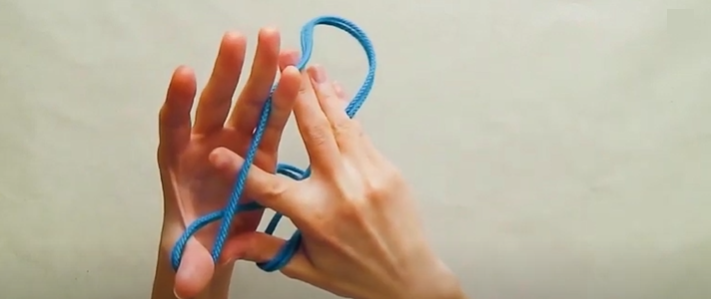
\includegraphics[width=0.81\linewidth]{3a}
		
		\vspace*{1pt}
		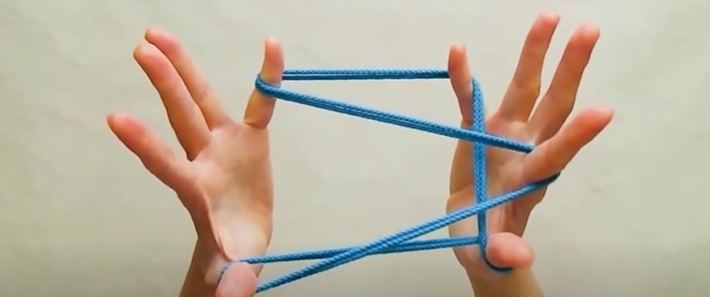
\includegraphics[width=0.81\linewidth]{3b}
			
		\vspace*{1pt}
		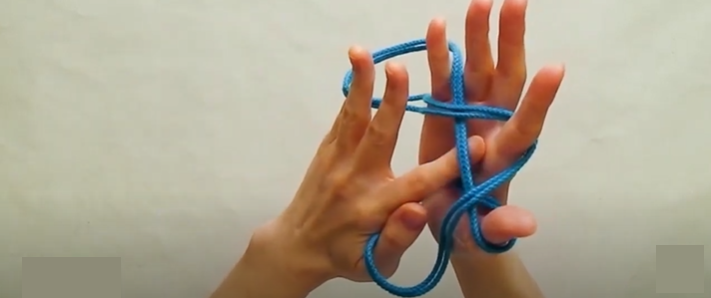
\includegraphics[width=0.81\linewidth]{3c}
				
		\vspace*{1pt}
		\hspace*{1pt}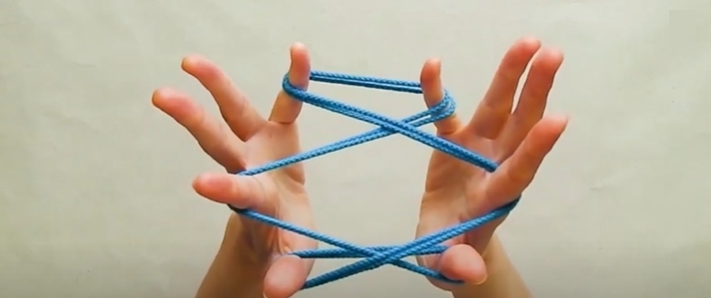
\includegraphics[width=0.81\linewidth]{3d}
		\vspace*{-10pt}
	\end{figure}
	\textit{Bước} $4$: Thả dây ở hai ngón tay út.
	\begin{figure}[H]
		\vspace*{-5pt}
		\centering
		\captionsetup{labelformat= empty, justification=centering}
		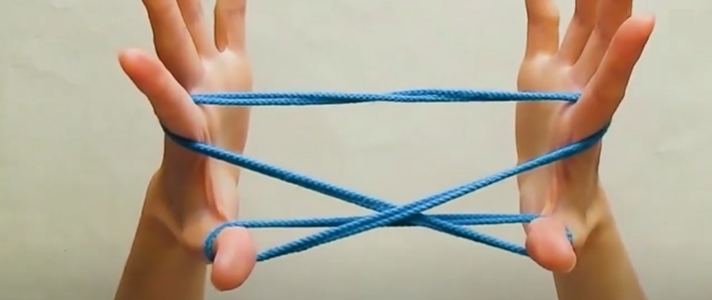
\includegraphics[width= 0.81\linewidth]{4}
		\vspace*{-10pt}
	\end{figure}
	\textit{Bước} $5$: Dùng ngón út để kéo sợi dây ở dưới cùng lên và chúng ta sẽ hoàn hành ngôi sao năm cánh.
	\begin{figure}[H]
		\vspace*{5pt}
		\centering
		\captionsetup{labelformat= empty, justification=centering}
		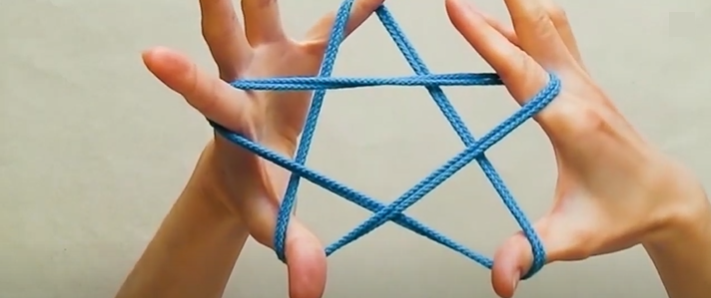
\includegraphics[width= 0.81\linewidth]{5}
		\vspace*{-5pt}
	\end{figure}
	Hãy thử suy ngẫm xem hình ngôi sao năm cánh em vừa tạo ra có bao nhiêu trục đối xứng?
	\vskip 0.1cm
	\textbf{\color{toancuabi}Làm cây thông Noel}
	\vskip 0.1cm
	\textit{Bước} $1$: Xếp hai tờ giấy màu cứng chồng lên nhau rồi gấp đôi lại cho đều nhau. Sau đó lấy bút vẽ phác họa hình cây thông lên mặt ngoài của tờ giấy rồi dùng kéo cắt theo các đường đã vẽ sẵn. Lúc mở ra, em sẽ có hai cây thông với kích thước giống nhau.
	\begin{figure}[H]
		\vspace*{-5pt}
		\centering
		\captionsetup{labelformat= empty, justification=centering}
		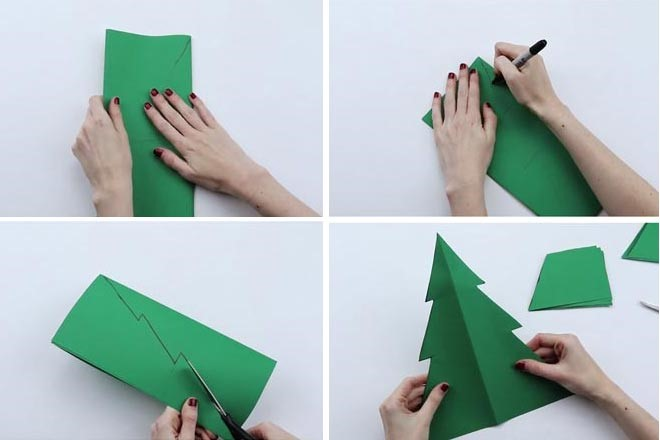
\includegraphics[width= 1\linewidth]{6}
		\vspace*{-15pt}
	\end{figure}
	\textit{Bước} $2$: Gấp đôi cây thông theo chiều ngang, gấp đầu nhọn xuống dưới để xác định tâm của mỗi cây thông. Tiếp đến dùng kéo cắt một đường từ đỉnh cây thông xuống điểm vừa đánh dấu. Cây thông còn lại thì cắt từ đáy lên điểm vừa đánh dấu.
	\begin{figure}[H]
		\vspace*{-5pt}
		\centering
		\captionsetup{labelformat= empty, justification=centering}
		\includegraphics[width= 1\linewidth]{7}
		\vspace*{-15pt}
	\end{figure}
	\textit{Bước} $3$: Sau khi đã hoàn thành việc cắt hai cây thông, em hãy ghép chúng lại với nhau theo các khe đã cắt, chú ý để các góc không bị cong. Nếu sau khi ráp cây thông bị lung lay các em có thể cố định lại bằng keo dán.
	\begin{figure}[H]
		\vspace*{-5pt}
		\centering
		\captionsetup{labelformat= empty, justification=centering}
		\includegraphics[width= 1\linewidth]{8}
		\vspace*{-15pt}
	\end{figure}
	\textit{Bước} $4$: Cuối cùng các em chỉ cần điều chỉnh sao cho cây thông đứng vững, trang trí thêm các dây ruy băng hay rắc kim tuyến,... hoặc vẽ họa tiết lên cây thông Noel để nhìn đẹp hơn.
	\begin{figure}[H]
		\vspace*{-5pt}
		\centering
		\captionsetup{labelformat= empty, justification=centering}
		\includegraphics[height= 0.31\linewidth]{9a}
		\includegraphics[height= 0.31\linewidth]{9b}
		\includegraphics[height= 0.31\linewidth]{9c}
		\caption{\small\textit{\color{toancuabi}Ảnh: Internet.}}
		\vspace*{-10pt}
	\end{figure}
	\textbf{\color{toancuabi}Bài tập}
	\vskip 0.1cm
	Còn gì tuyệt vời hơn khi được thả diều dưới bầu trời xanh và trong làn gió mát của những buổi chiều mùa hè oi ả. Bằng những kiến thức của bài ``Hình có trục đối xứng" và trí tưởng tượng phong phú của mình, em hãy tự làm ra cho mình một con diều đẹp đẽ với màu sắc rực rỡ nhé. Chúc em thành công!
	\begin{figure}[H]
			\vspace*{-5pt}
			\centering
			\captionsetup{labelformat= empty, justification=centering}
			\includegraphics[width= 1\linewidth]{10}
			\caption{\small\textit{\color{toancuabi}Hình ảnh con diều (Ảnh: Internet)}}
			\vspace*{-5pt}
		\end{figure}
\end{multicols}